\section{Experimental evaluations} \label{sec:experiments}

We assess the predictive greedy algorithms in real-world applications: ML feature selection, influence maximization, and text summarization. Extensive experiments are conducted with real-world datasets to evaluate the algorithms against benchmarks. Code can be found \cite{anonymous2024submodularexperiment}. 

The experiment aims to evaluate the proposed framework of submodular optimization with predictions on real-world applications, where the submodularity of the objective is assumed rather than guaranteed. The objective often empirically captures submodularity but is not strictly submodular. For example, in ML feature selection, information coverage of a set of features is submodular, but the end goal is out-of-sample predictive performance, which relies on information coverage but might not necessarily be submodular. We will compare our algorithm with existing benchmarks and assess its consistency, smoothness, and robustness. Our study will not compute the optimal solution directly, as it is computationally infeasible where no polynomial-time algorithm exists \cite{setCoverisHard}, but we will compare against an upper bound of the optimum to show differences between theoretical and empirical performance ratios. 
%\textcolor{purple}{At the same time, we focus on the predictive algorithm's comparative performance instead of determining the exact approximation ratio.}



\begin{figure*}[ht]
    \centering
    % First figure
    \begin{minipage}{0.24\textwidth}
        \centering
        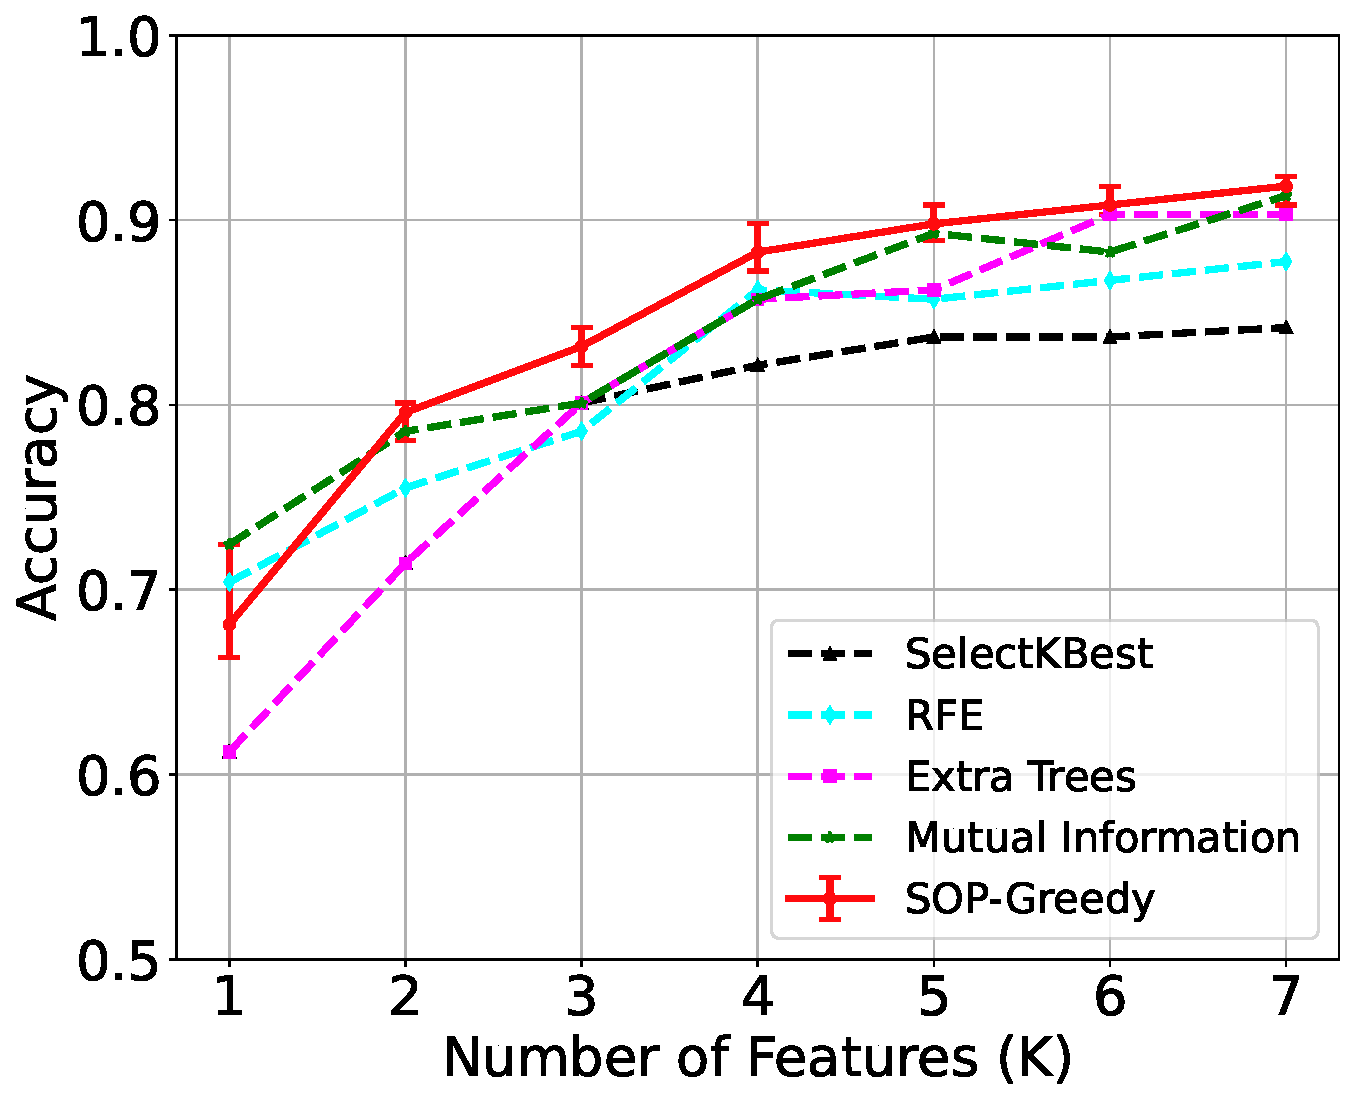
\includegraphics[width=\linewidth]{Figures/experiment 1/predictive_performance_airline3.pdf}
        %\\{\tiny (a)}
        \label{fig:airline_performance}
    \end{minipage}\hfill
    % Second figure
    \begin{minipage}{0.24\textwidth}
        \centering
        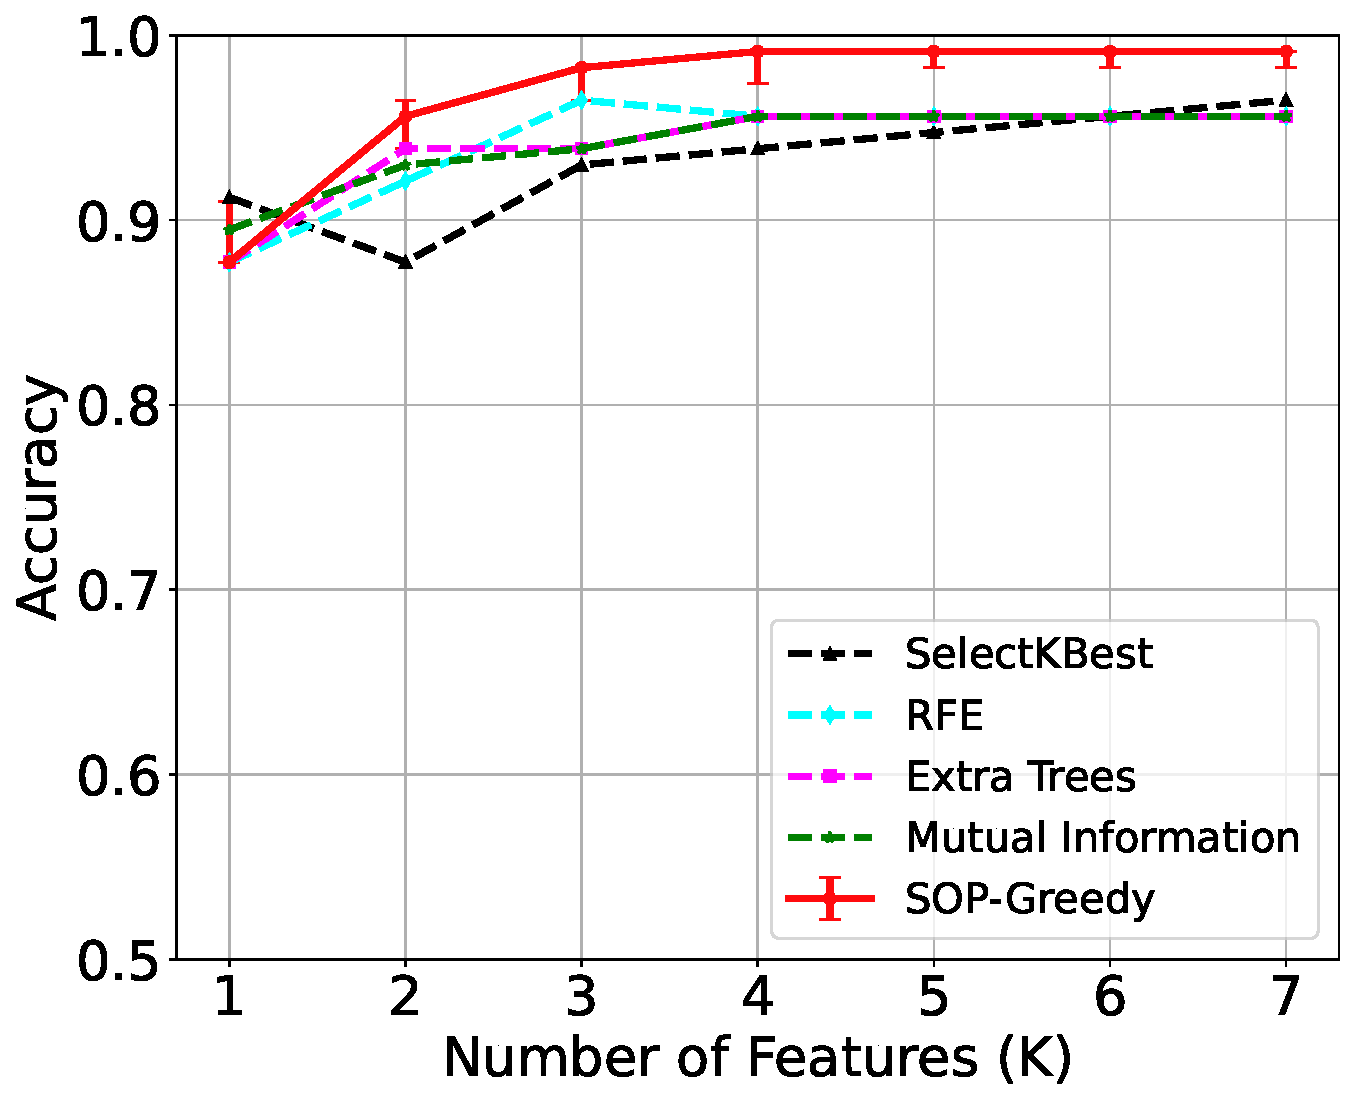
\includegraphics[width=\linewidth]{Figures/experiment 1/predictive_performance3.pdf}
        %\\{\tiny (b)}
        \label{fig:cancer_performance}
    \end{minipage}
    \hfill
    % Third figure
    \begin{minipage}{0.24\textwidth}
        \centering
        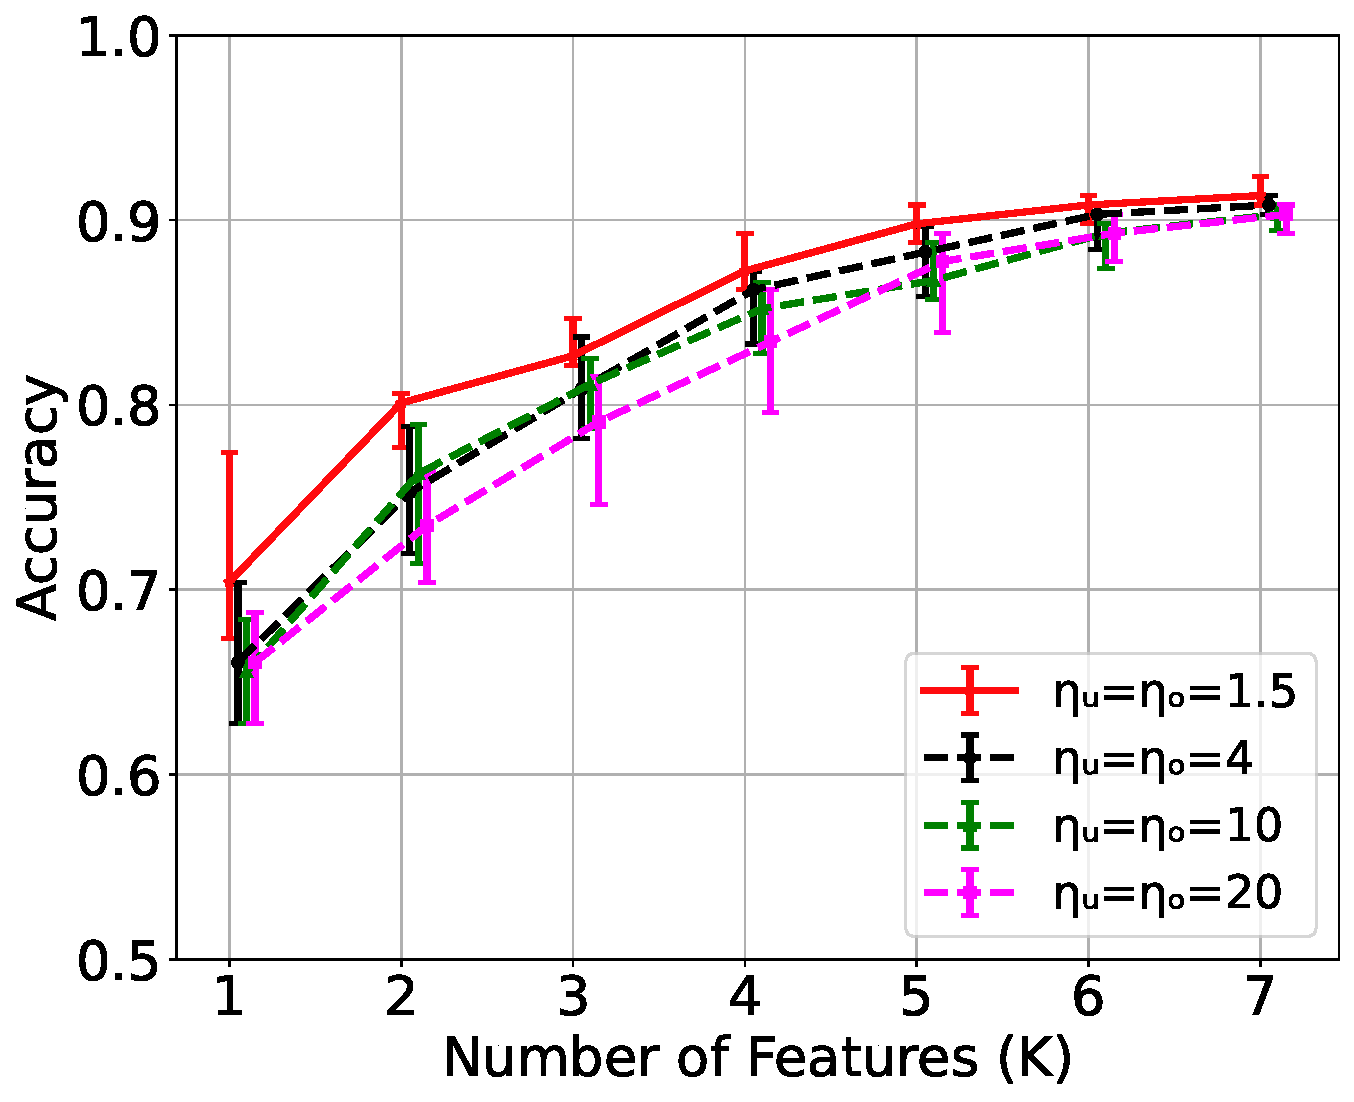
\includegraphics[width=\linewidth]{Figures/experiment 1/eta_airline_performance4.pdf}
        %\\{\tiny (c)}
        \label{fig:eta_airline}
    \end{minipage}
    \hfill
    % Fourth figure
    \begin{minipage}{0.24\textwidth}
        \centering
        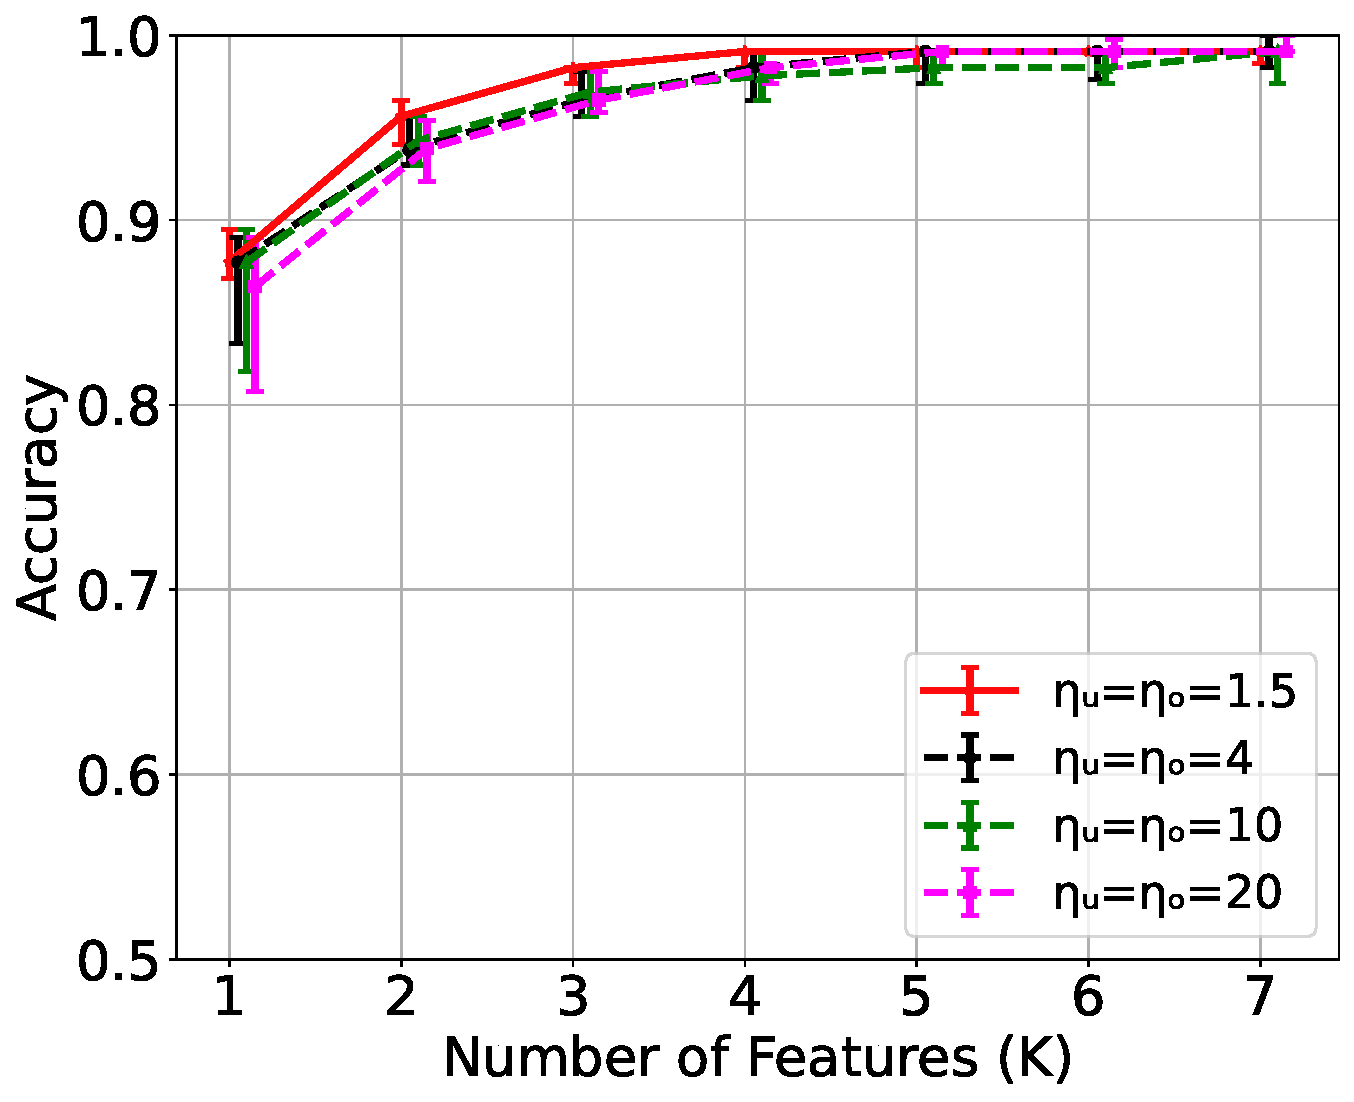
\includegraphics[width=\linewidth]{Figures/experiment 1/eta_cancer_performance2.pdf}
        %\\{\tiny (d)}
        \label{fig:eta_cancer}
    \end{minipage}

    \caption{The oos accuracy of Submodular Optimization Predictive Greedy (SOP-Greedy), with $R = 1$ and $\eta_o = \eta_u = 1.5$, against four benchmarks and under different prediction errors. From left to right, the first two figures are under an increasing $K$ for the airline passenger satisfaction and breast cancer datasets. The last two are the performance of SOP-Greedy under an increasing $\eta$, from 2.25 to 400, for the two tasks.}
    \label{fig:experiment1-performance}
    \vspace{-10pt}
\end{figure*}

% \footnote{https://anonymous.4open.science/r/SubmodularExperiment-DB09/}}
\begin{figure}
    \centering
    % First figure
    \begin{minipage}{0.42\textwidth}
        \centering
        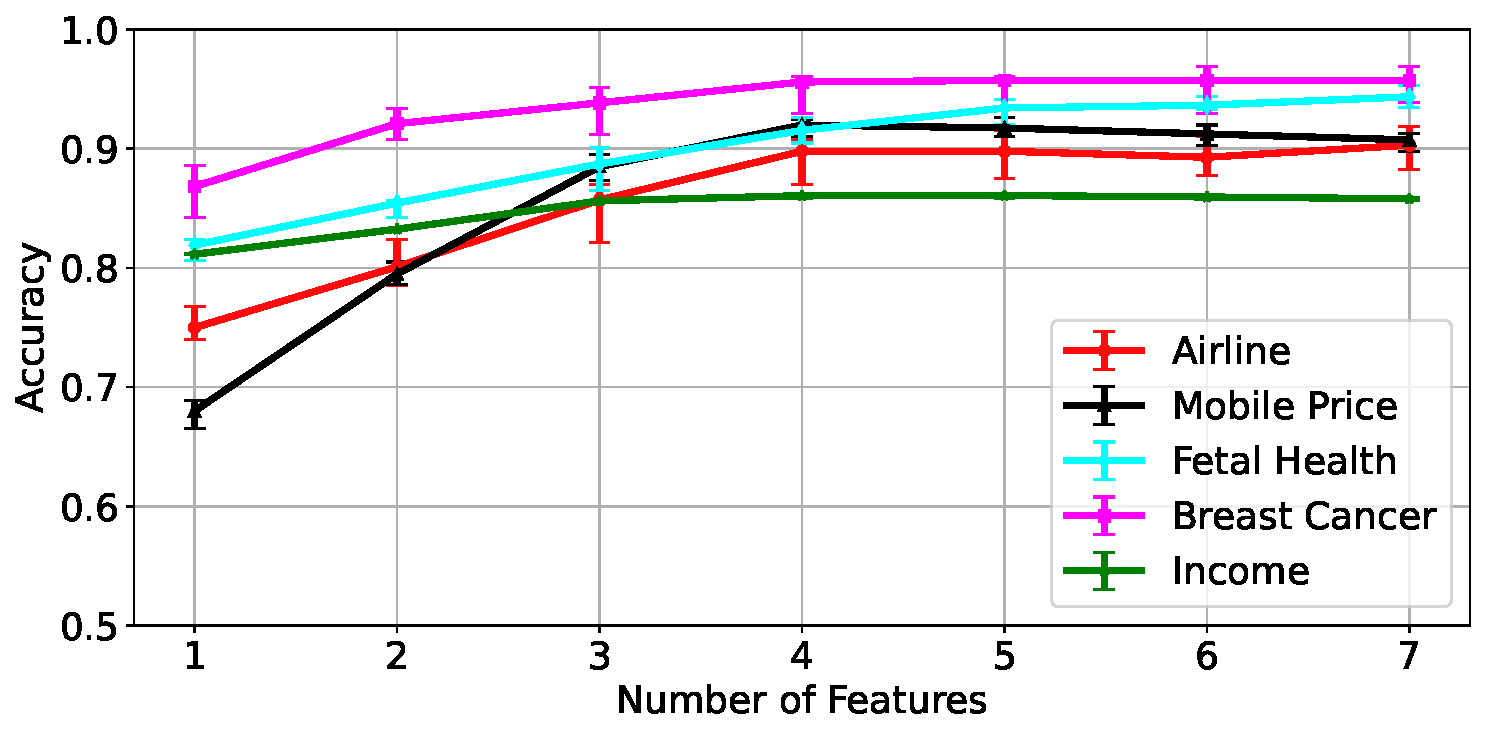
\includegraphics[width=\linewidth]{Figures/experiment 1/combined_submodular_proof (1).pdf}
        %\\{\tiny (a)}
    \end{minipage}\hfill
    
    \caption{Empirical evidence of the approximate submodularity for oos accuracy as a function of the number of features verified on five real-world classification datasets \cite{Salini2024,Kalaivani2021,Chakraborty2020}. We run a greedy feature selection and measure the additivity of each feature. The overall accuracy increases when features are added with clear diminishing returns.}
    \label{fig:submod}
    \vspace{-12pt}
\end{figure}





\begin{figure}[t]
    \centering
    % First figure
    \begin{minipage}{0.45\textwidth}
        \centering
        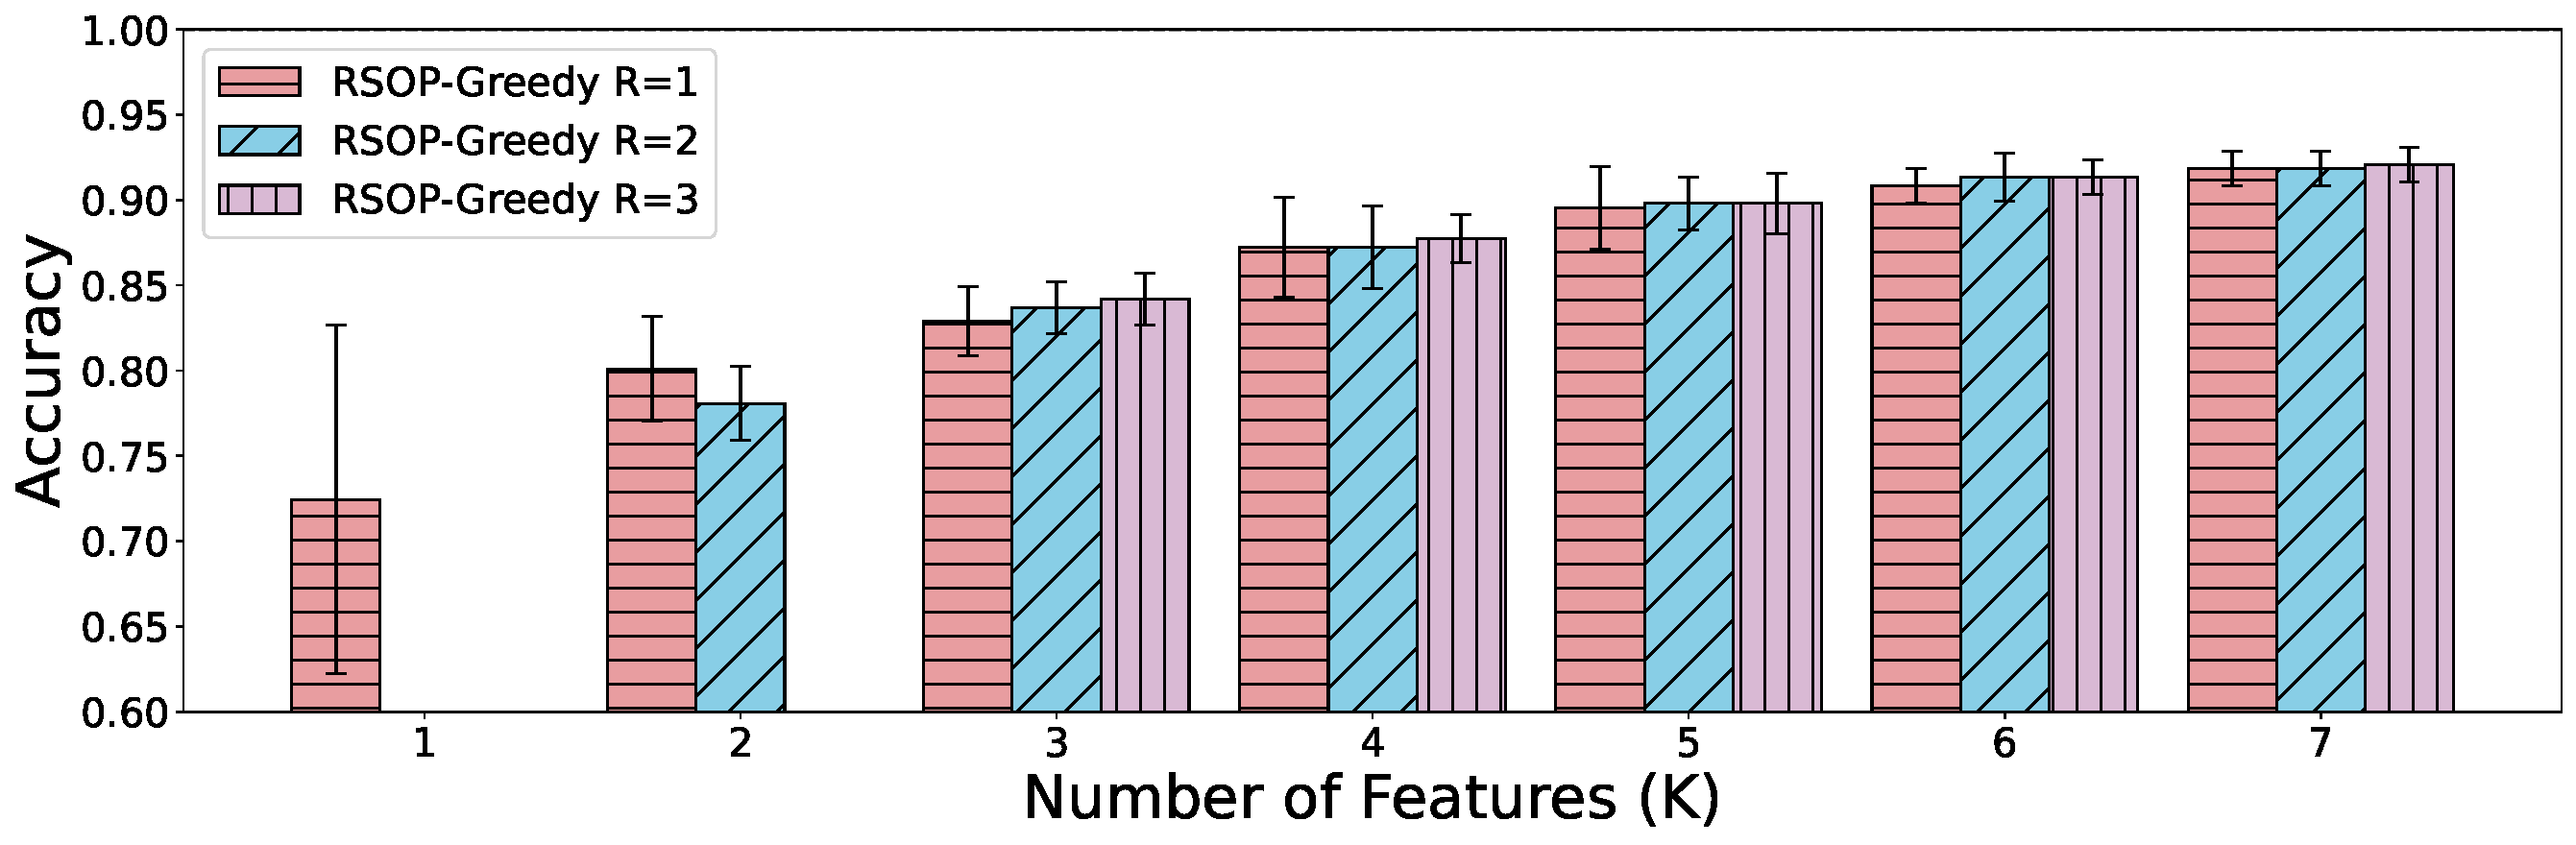
\includegraphics[width=\linewidth]{Figures/experiment 1/r_airline.pdf}
        %\\{\tiny (a)}
        \label{fig:airline_performance_R_step}
    \end{minipage}\hfill
    % Second figure
    \begin{minipage}{0.44\textwidth}
        \centering
        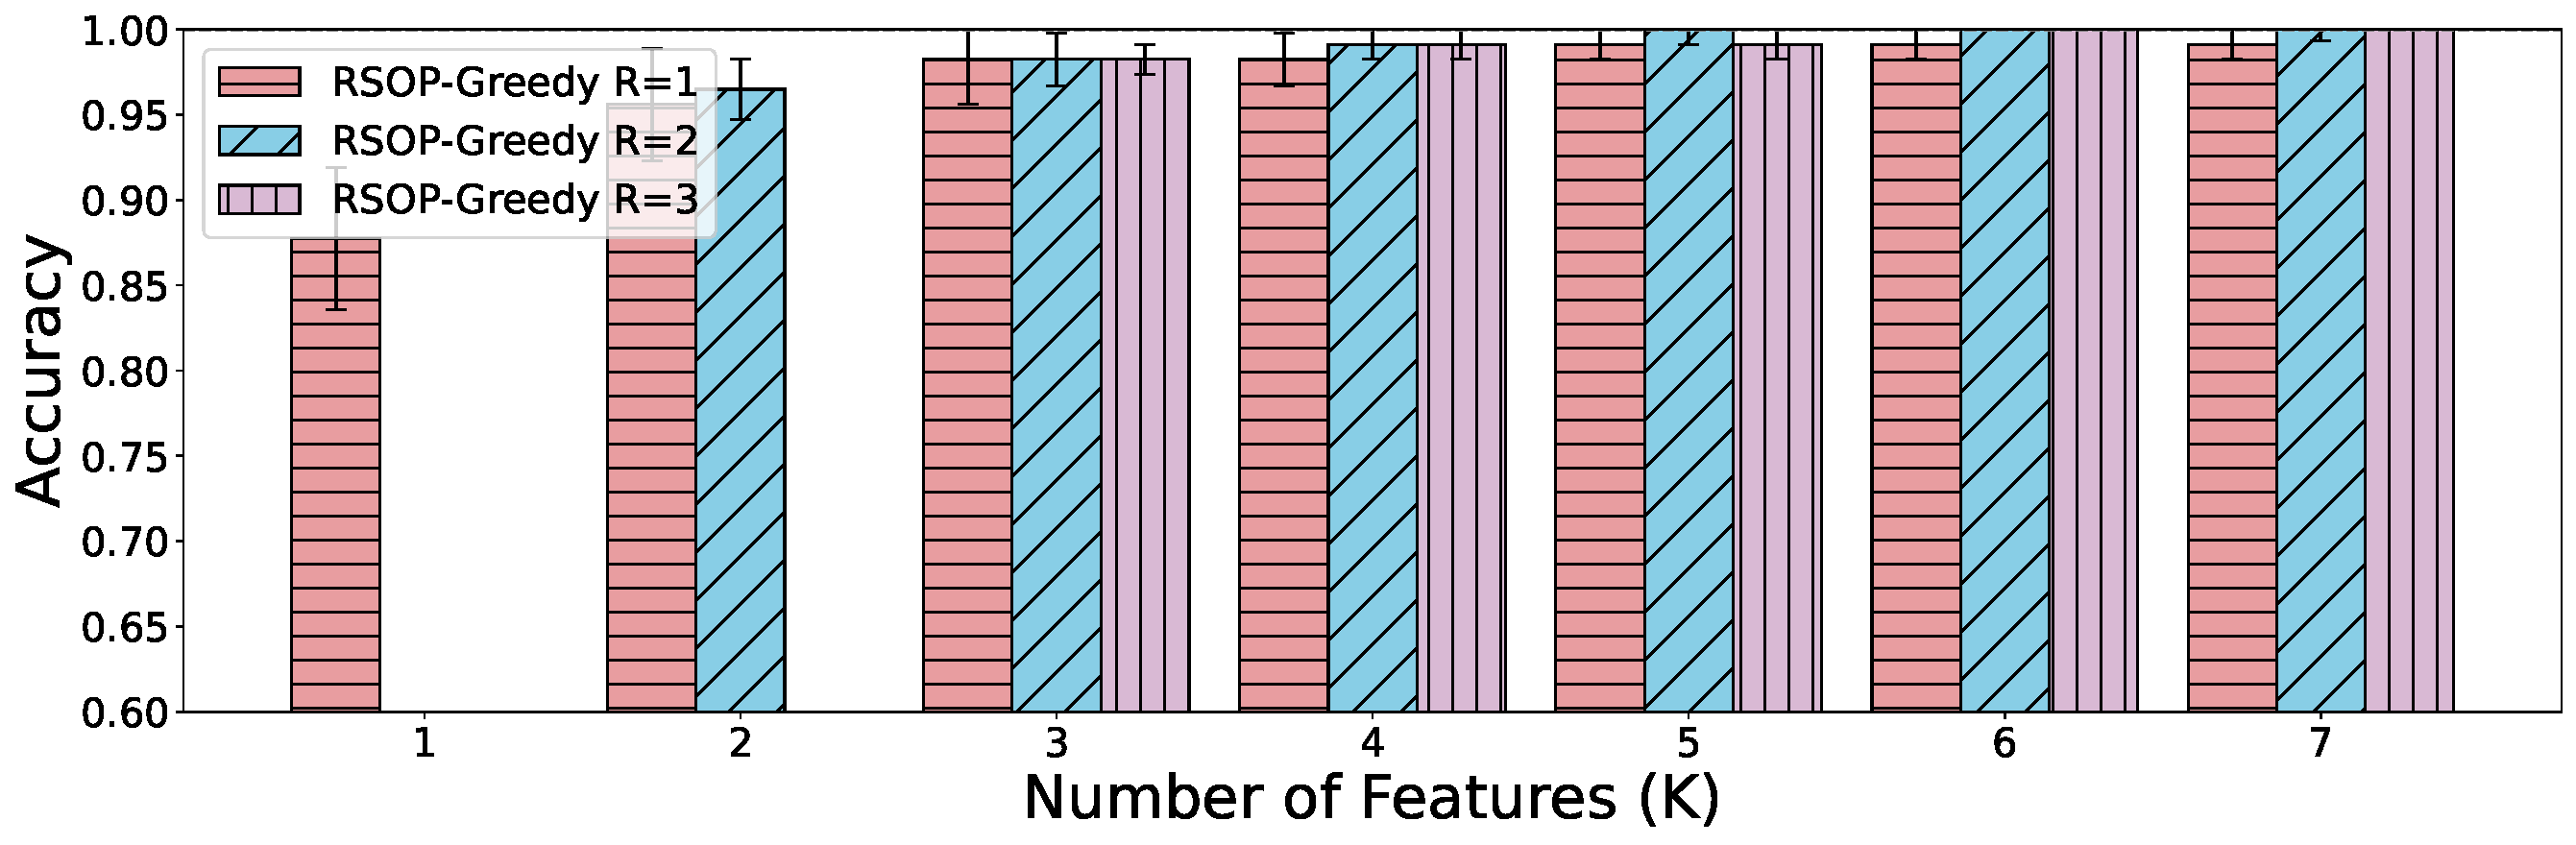
\includegraphics[width=\linewidth]{Figures/experiment 1/r_cancer.pdf}
        %\\{\tiny (b)}
        \label{fig:predictive_performance}
    \end{minipage}

    \caption{The oos accuracy of the R-step Greedy (RSOP-Greedy) with $R = 1, 2, 3$ and $\eta_o = \eta_u = 1.5$. From left to right, the figures present the accuracy with different $K$ for the airline and breast cancer datasets.}
    \label{fig:experiment2-R-step}
    \vspace{-6pt}
\end{figure}

\vspace{-10pt}
\subsection{ML feature selection} \label{subsec:feature-selection}


% Pose the application as submodular optimization
Supervised learning aims at predictive models that perform well on \textit{out-of-sample (oos)} data. Given training data $\boldsymbol{X}$ with $n$ feature columns labeled as $1, ..., n$ and a target vector $y$, our task is to find features $S \subseteq [n]$, subject to $|S| \leq K$ for a given $K$, for model $h(\boldsymbol{Y}[S]; \boldsymbol{\theta})$, where $S \subseteq [n]$, $\boldsymbol{Y}[S]$ denotes data $\boldsymbol{Y}$ with columns $S$, and $\boldsymbol{\theta}$ the model parameters depending on $S$. The model's performance is defined by function $\mathcal{L}$ on some oos data $\boldsymbol{Z}$ and a target vector $w$, denoted by $\mathcal{L}(h(\boldsymbol{Z}[S]; \boldsymbol{\theta}), w)$. We assume a given training process $p$ that determines $\boldsymbol{\theta}$ given $\boldsymbol{X}$, $y$, and $S$. The ML feature selection problem can be cast as: 
\[ \max_{S \subseteq [n]}\{ \mathcal{L}(h(\boldsymbol{Z}[S]; p(\boldsymbol{X}, y, S)), w): |S| \leq K\} \]
where $\mathcal{L}$, $h$, $p$, $\boldsymbol{X}$, $y$, and $K$ are known, $\boldsymbol{Z}$ and $w$ are not, and $S$ is the decision variable. Let $f(S) = \mathcal{L}(h(\boldsymbol{Z}[S]; p(\boldsymbol{X}, y, S)), w)$. Function $f$ may not be strictly submodular, but has observed diminishing gains in adding features due to feature correlation \cite{wei2014submodular}. This empirical observation is verified in various learning tasks shown in Figure \ref{fig:submod}. Thus, $f$ is assumed to be submodular. We cannot access $f$, but we assume a predictor $\tilde{f}$ for $f$ is accessible, allowing us to query $\tilde{d}_B(A)$ for any $A, B \subseteq [n]$.
% Give experimental set-up: how our algorithm is implemented, what are the benchmarks

\begin{table}[ht!]
\centering
\caption{Empirical ratios of RSOP-Greedy with different $R$ (estimated assuming $\mathrm{OPT}=1$) in the airline dataset and their theoretical bounds ($\eta=2.25$).}
\label{tab:airline-r-steps-theo}
\begin{tabular}{c|ccccccc}
\hline\hline
\textbf{R} 
& \textbf{K=1} & \textbf{K=2} & \textbf{K=3} & \textbf{K=4} & \textbf{K=5} & \textbf{K=6} & \textbf{K=7}\\
\hline
{\textbf{1}} 
  & 0.725 & 0.801 & 0.829 & 0.872 & 0.895 & 0.908 & 0.918 \\[-3pt]
  & (0.444) & (0.395) & (0.382) & (0.376) & (0.371) & (0.369) & (0.366) \\
{\textbf{2}}
  & ---   & 0.781 & 0.837 & 0.872 & 0.898 & 0.913 & 0.918 \\[-3pt]
  & (0.444) & (0.444) & (0.395) & (0.395) & (0.382) & (0.382) & (0.376) \\
{\textbf{3}}
  & ---   & ---   & 0.842 & 0.878 & 0.898 & 0.913 & 0.921 \\[-3pt]
  & (0.444) & (0.444) & (0.444) & (0.395) & (0.395) & (0.395) & (0.382) \\
\hline\hline
\end{tabular}
\vspace{-5pt}
\end{table}

\begin{table}[ht!]
\centering
\caption{Empirical ratios of RSOP-Greedy in the breast cancer dataset and their theoretical bounds ($\eta=2.25$).}
\label{tab:breast-r-steps-theo}
\begin{tabular}{c|ccccccc}
\hline\hline
\textbf{R} 
& \textbf{K=1} & \textbf{K=2} & \textbf{K=3} & \textbf{K=4} & \textbf{K=5} & \textbf{K=6} & \textbf{K=7}\\
\hline
{\textbf{1}} 
  & 0.877 & 0.965 & 0.983 & 0.991 & 0.991 & 0.991 & 0.991 \\[-3pt]
  & (0.444) & (0.395) & (0.382) & (0.376) & (0.371) & (0.369) & (0.366) \\
{\textbf{2}}
  & ---    & 0.956 & 0.991 & 0.991 & 0.983 & 1.000 & 1.000 \\[-3pt]
  & (0.444) & (0.444) & (0.395) & (0.395) & (0.382) & (0.382) & (0.376) \\
{\textbf{3}}
  & ---    & ---    & 0.974 & 0.991 & 1.000 & 1.000 & 1.000 \\[-3pt]
  & (0.444) & (0.444) & (0.444) & (0.395) & (0.395) & (0.395) & (0.382) \\
\hline\hline
\end{tabular}
%\vspace{-12pt}
\end{table}

\begin{figure*}[t!]
    \centering
    % First figure
    \begin{minipage}{0.245\textwidth}
        \centering
        
\includegraphics[width=\linewidth]{Figures/experiment 2/new/n_twt.pdf}
        \label{fig:2stp_twt}
    \end{minipage}\hfill
    % Second figure
    \begin{minipage}{0.245\textwidth}
        \centering
        
\includegraphics[width=\linewidth]{Figures/experiment 2/new/n_rdt.pdf}
        \label{fig:2stp_rdt}
    \end{minipage}
    \hfill
    % Third figure
    \begin{minipage}{0.245\textwidth}
        \centering
        
\includegraphics[width=\linewidth]{Figures/experiment 2/new/n_fb1.pdf}
        \label{fig:2stp_fb1}
    \end{minipage}
    \hfill
    % Fourth figure
    \begin{minipage}{0.245\textwidth}
        \centering
        
\includegraphics[width=\linewidth]{Figures/experiment 2/new/n_fb2.pdf}
        \label{fig:2stp_fb2}
    \end{minipage}

    \caption{Performance ratio with an increasing $K$. We retain 1000 nodes for each dataset for reasonable run-time of RSOP-Greedy. 
    % Results on the full networks (excluding RSOP-Greedy) are in the Appendix E.
    %\ref{appendix:large-scale}.
    }
    \label{fig:2stp}
\end{figure*}






\begin{figure*}[t!]
    \centering
    % First figure
    \begin{minipage}{0.19\textwidth}
        \centering
        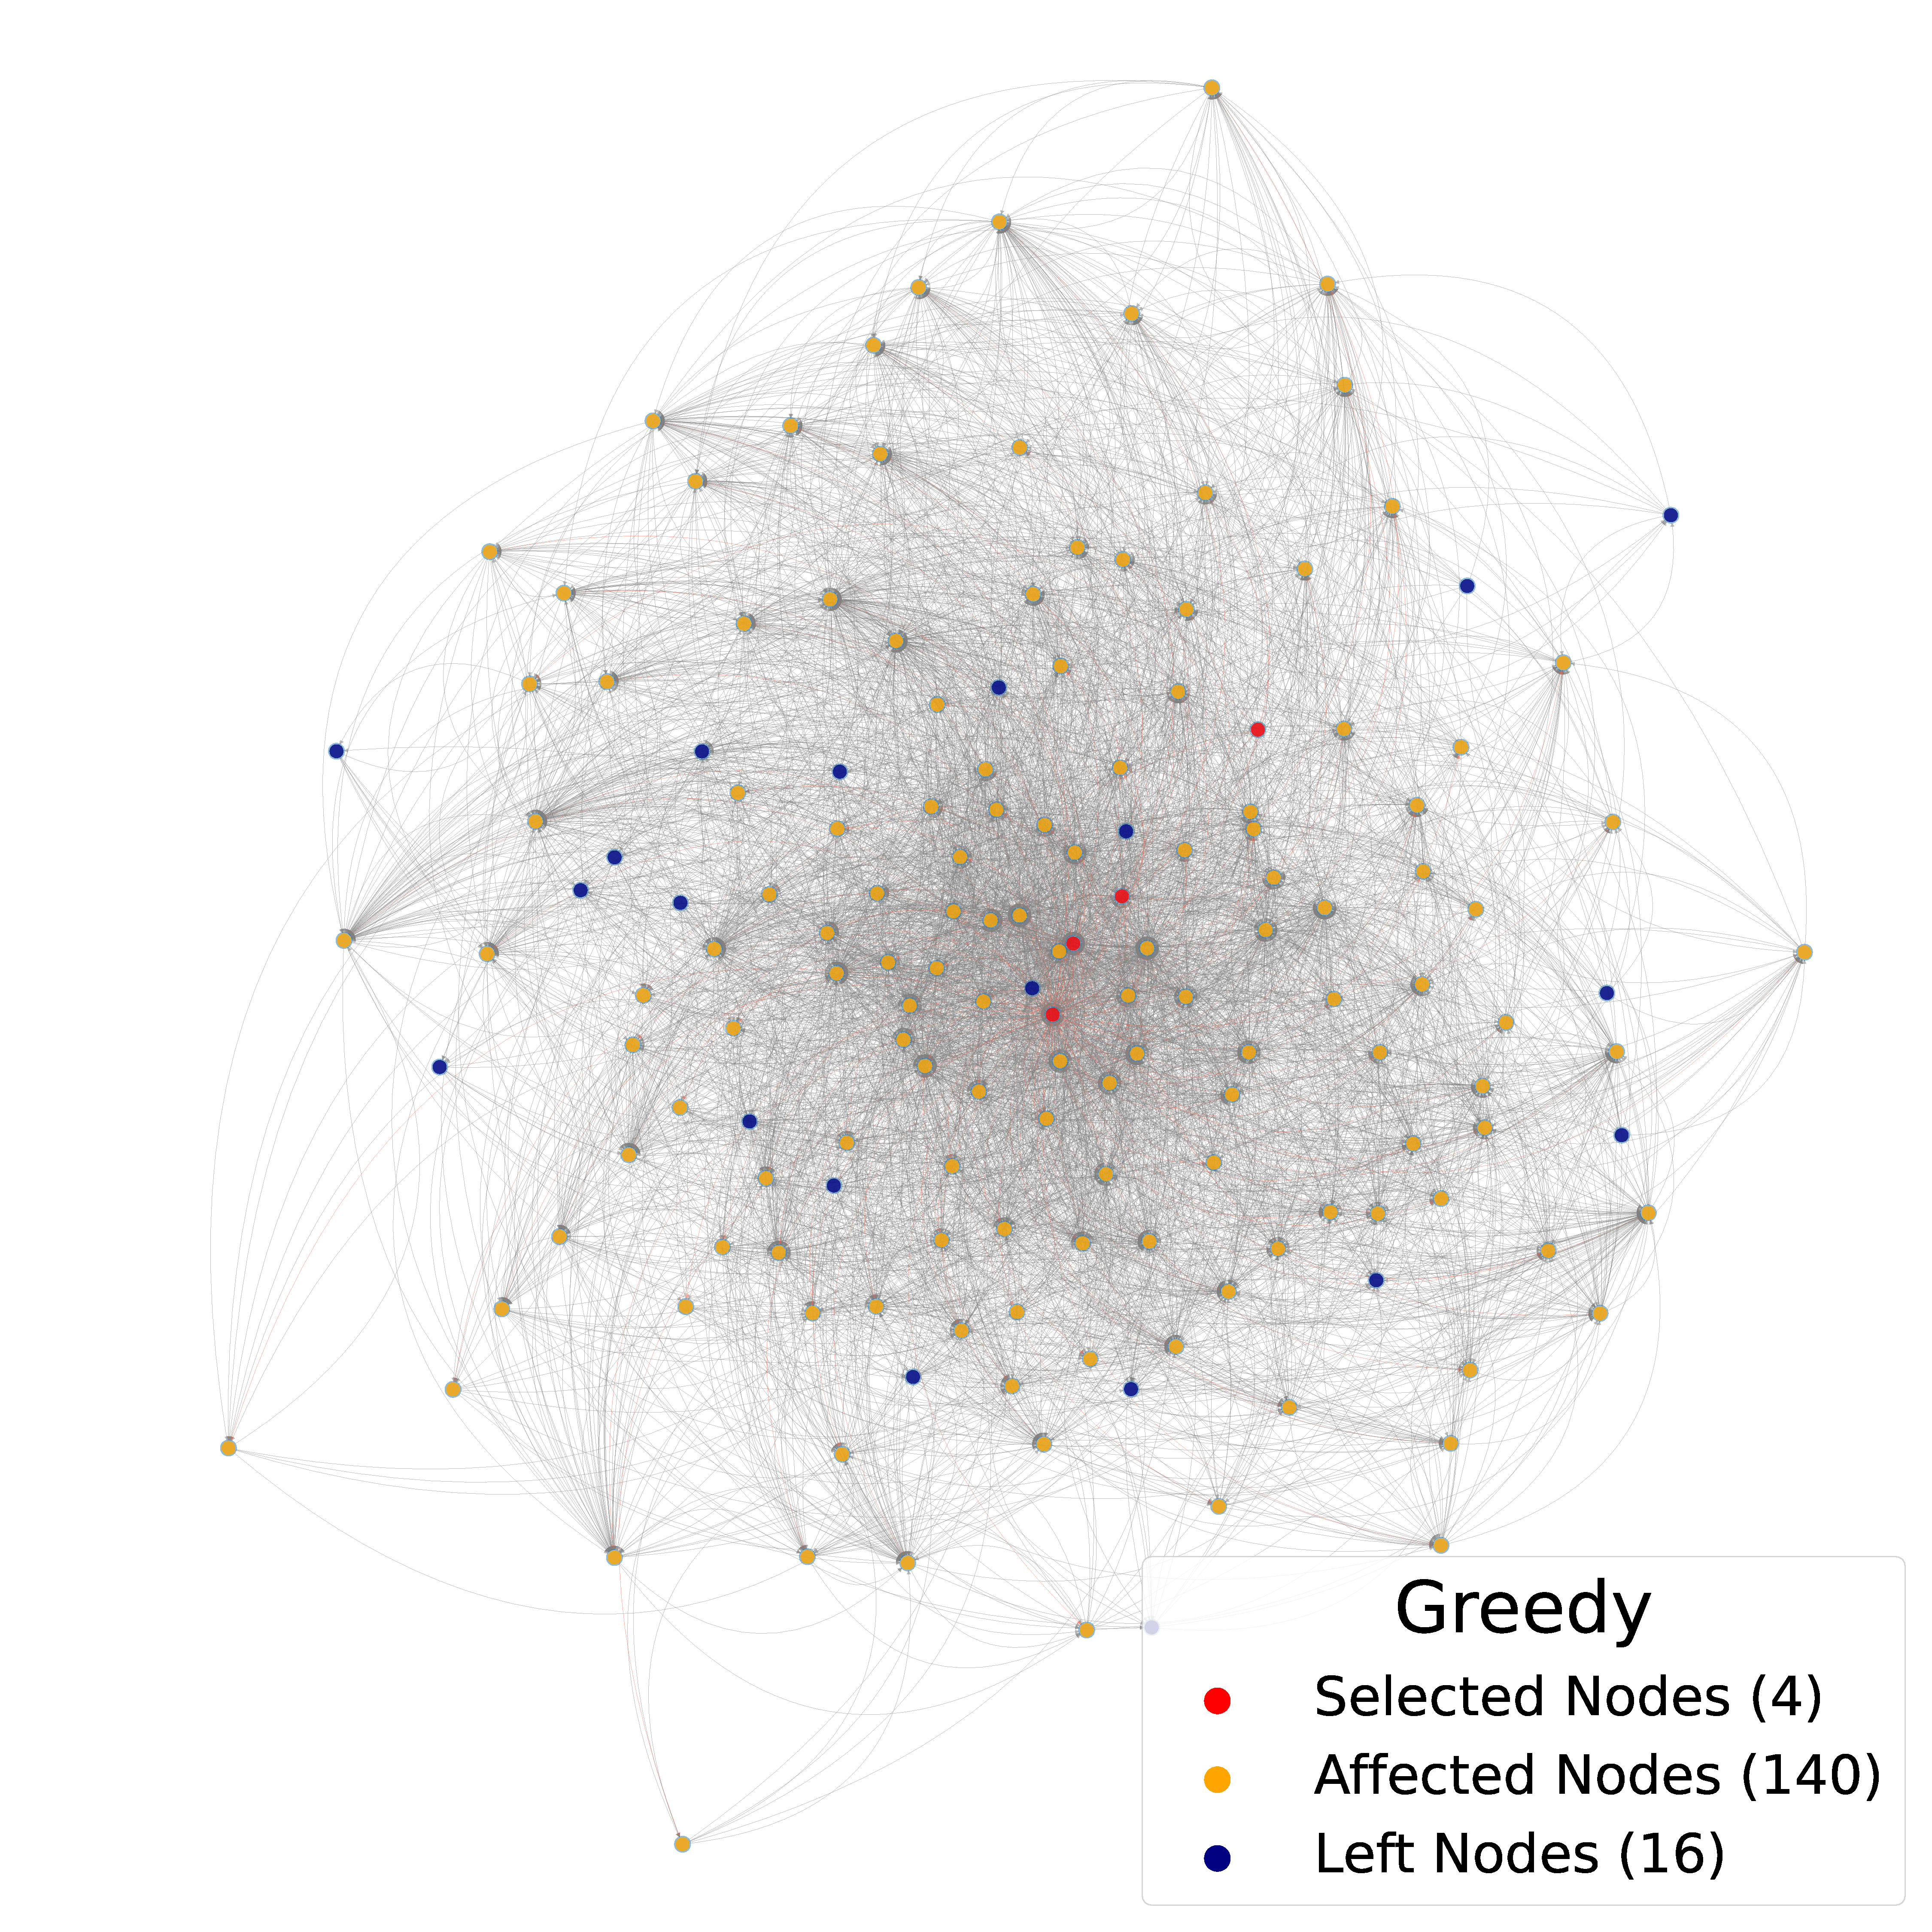
\includegraphics[width=\linewidth]{Figures/GraphExperiment/Network/plot_Greedy.pdf}
        %\\{\tiny Greedy}
        \label{fig:g}
    \end{minipage}%\hspace{0.005\textwidth}
    \hfill
    % Second figure
    \begin{minipage}{0.19\textwidth}
        \centering
        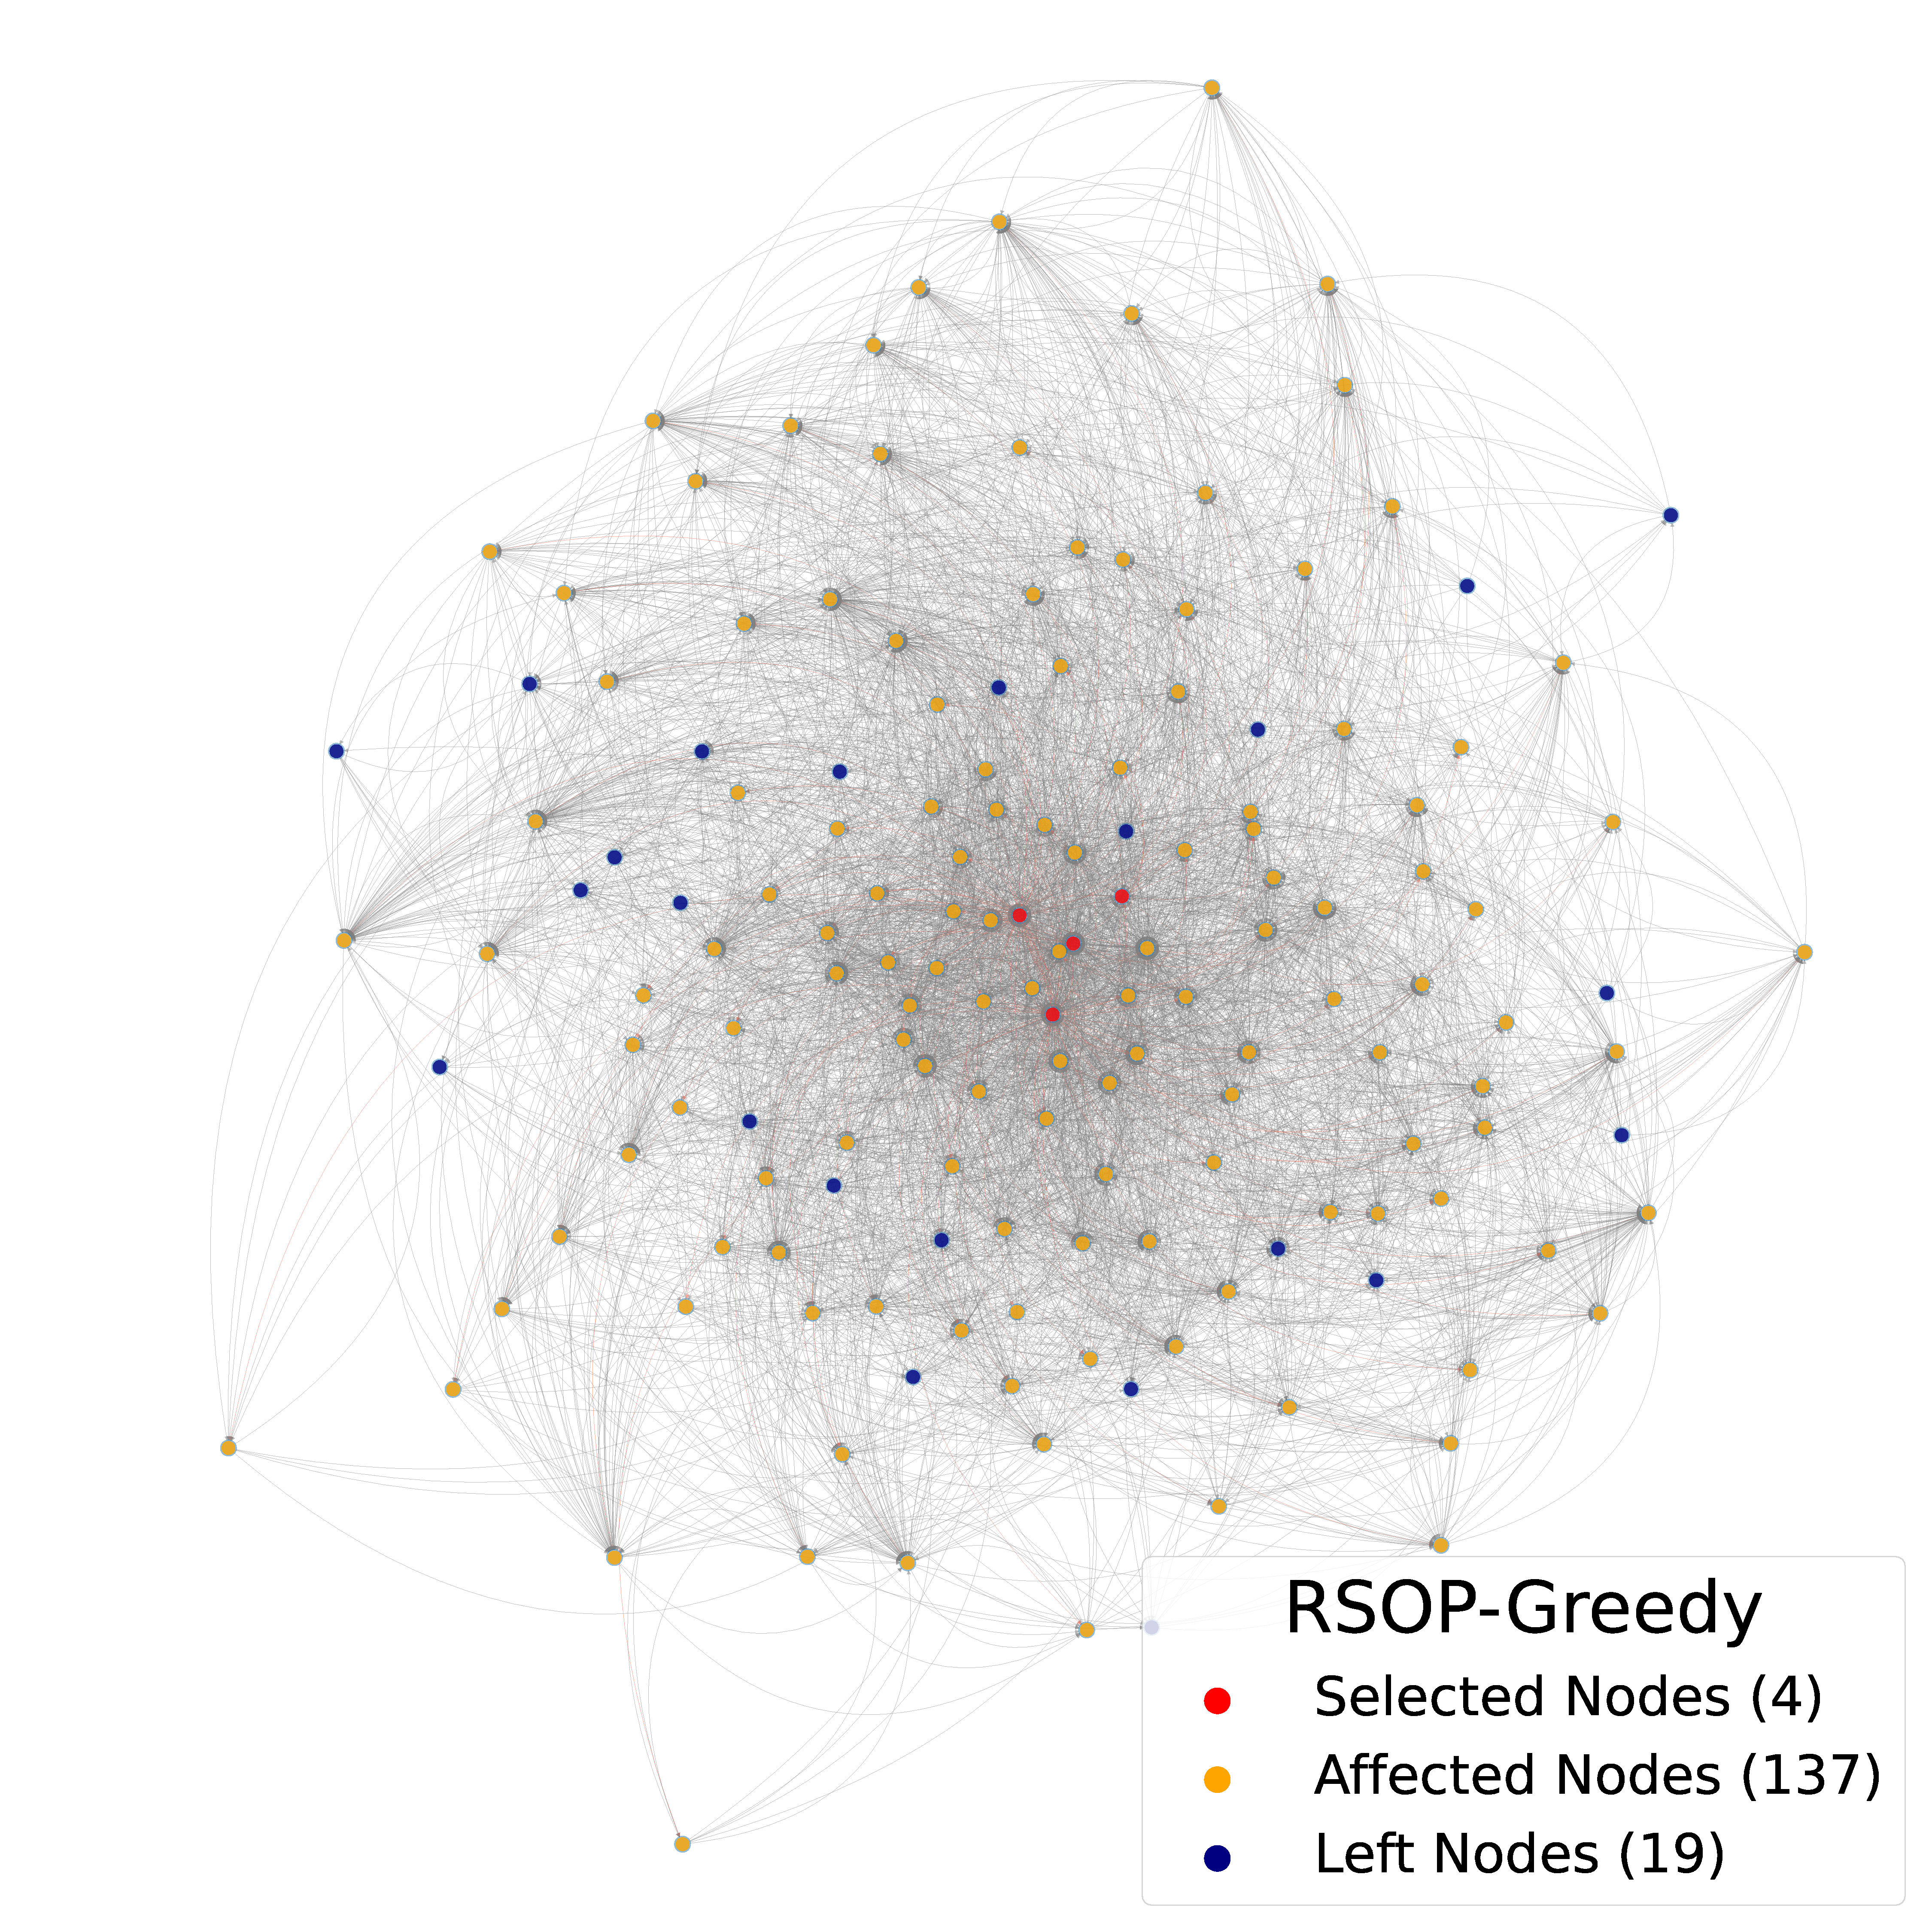
\includegraphics[width=\linewidth]{Figures/GraphExperiment/Network/plot_RSOP-Greedy.pdf}
        %\\{\tiny SOP-Greedy}
        \label{fig:sop}
    \end{minipage}%\hspace{0.005\textwidth}
    \hfill
    % Third figure
    \begin{minipage}{0.19\textwidth}
        \centering
        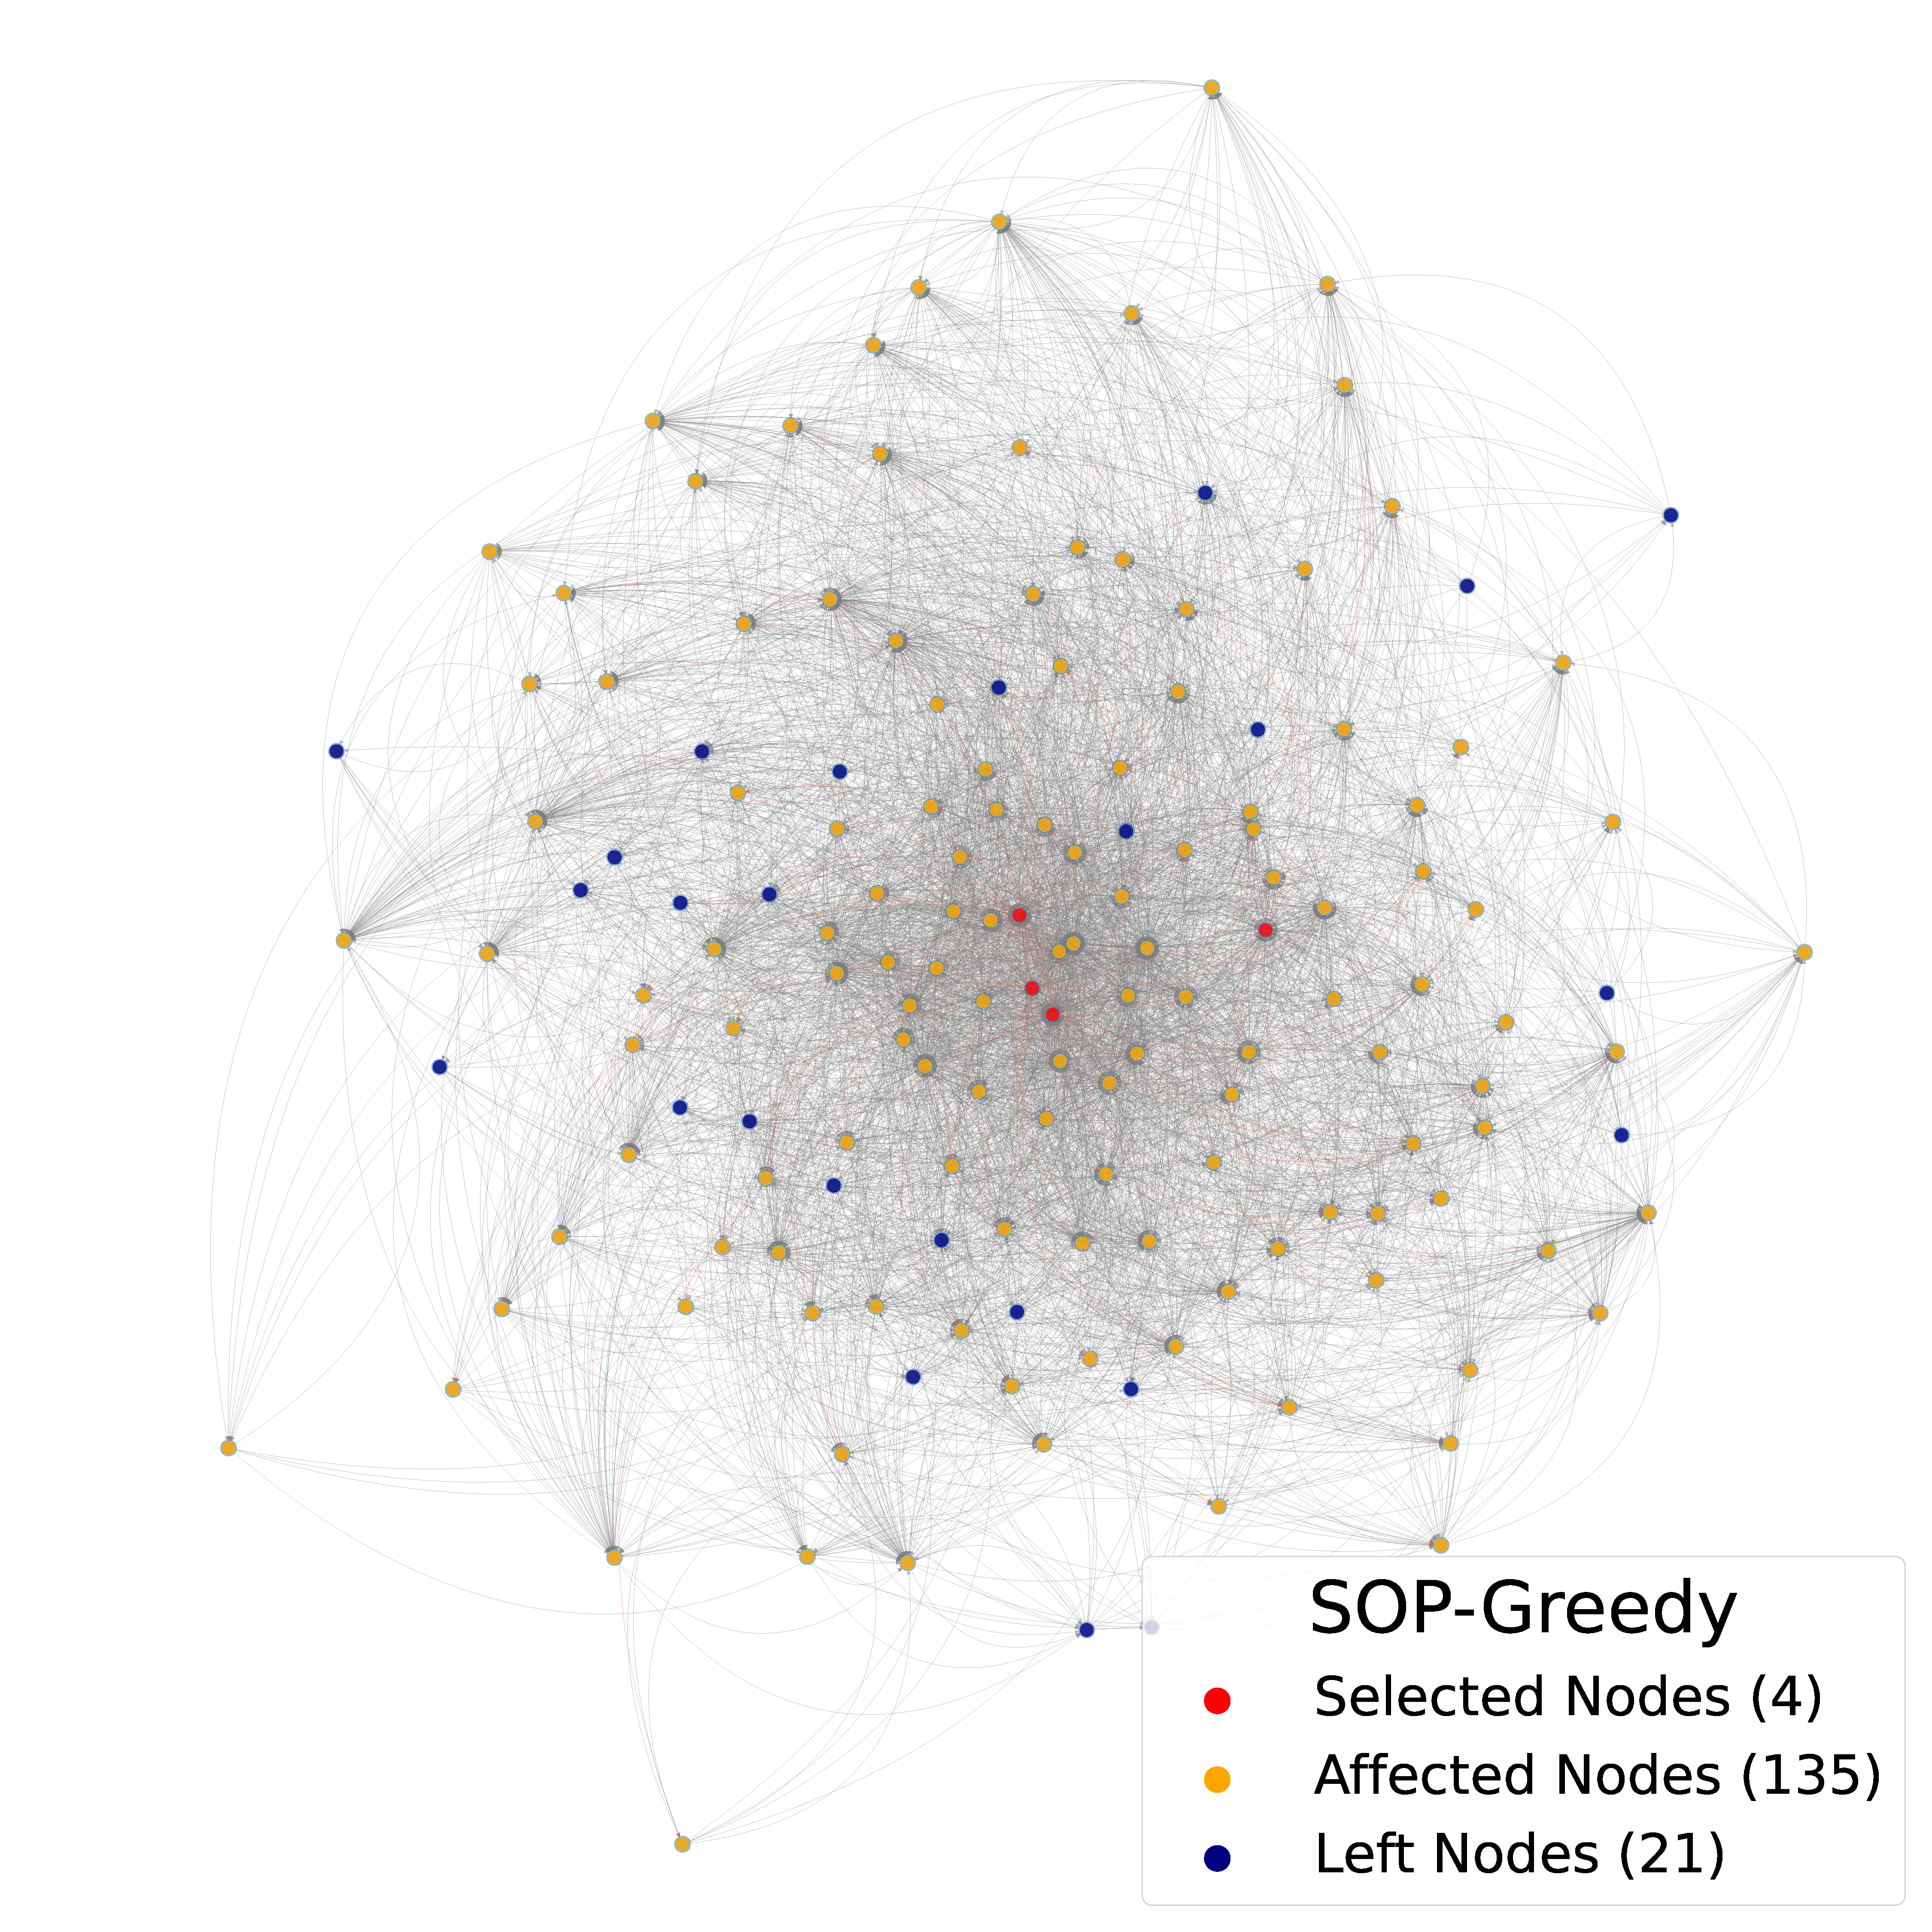
\includegraphics[width=\linewidth]{Figures/GraphExperiment/Network/plot_SOP-Greedy.pdf}
        %\\{\tiny RSOP-Greedy ($R = 2$)}
        \label{fig:rsop}
    \end{minipage}%\hspace{0.005\textwidth}
    \hfill
    % Fourth figure
    \begin{minipage}{0.19\textwidth}
        \centering
        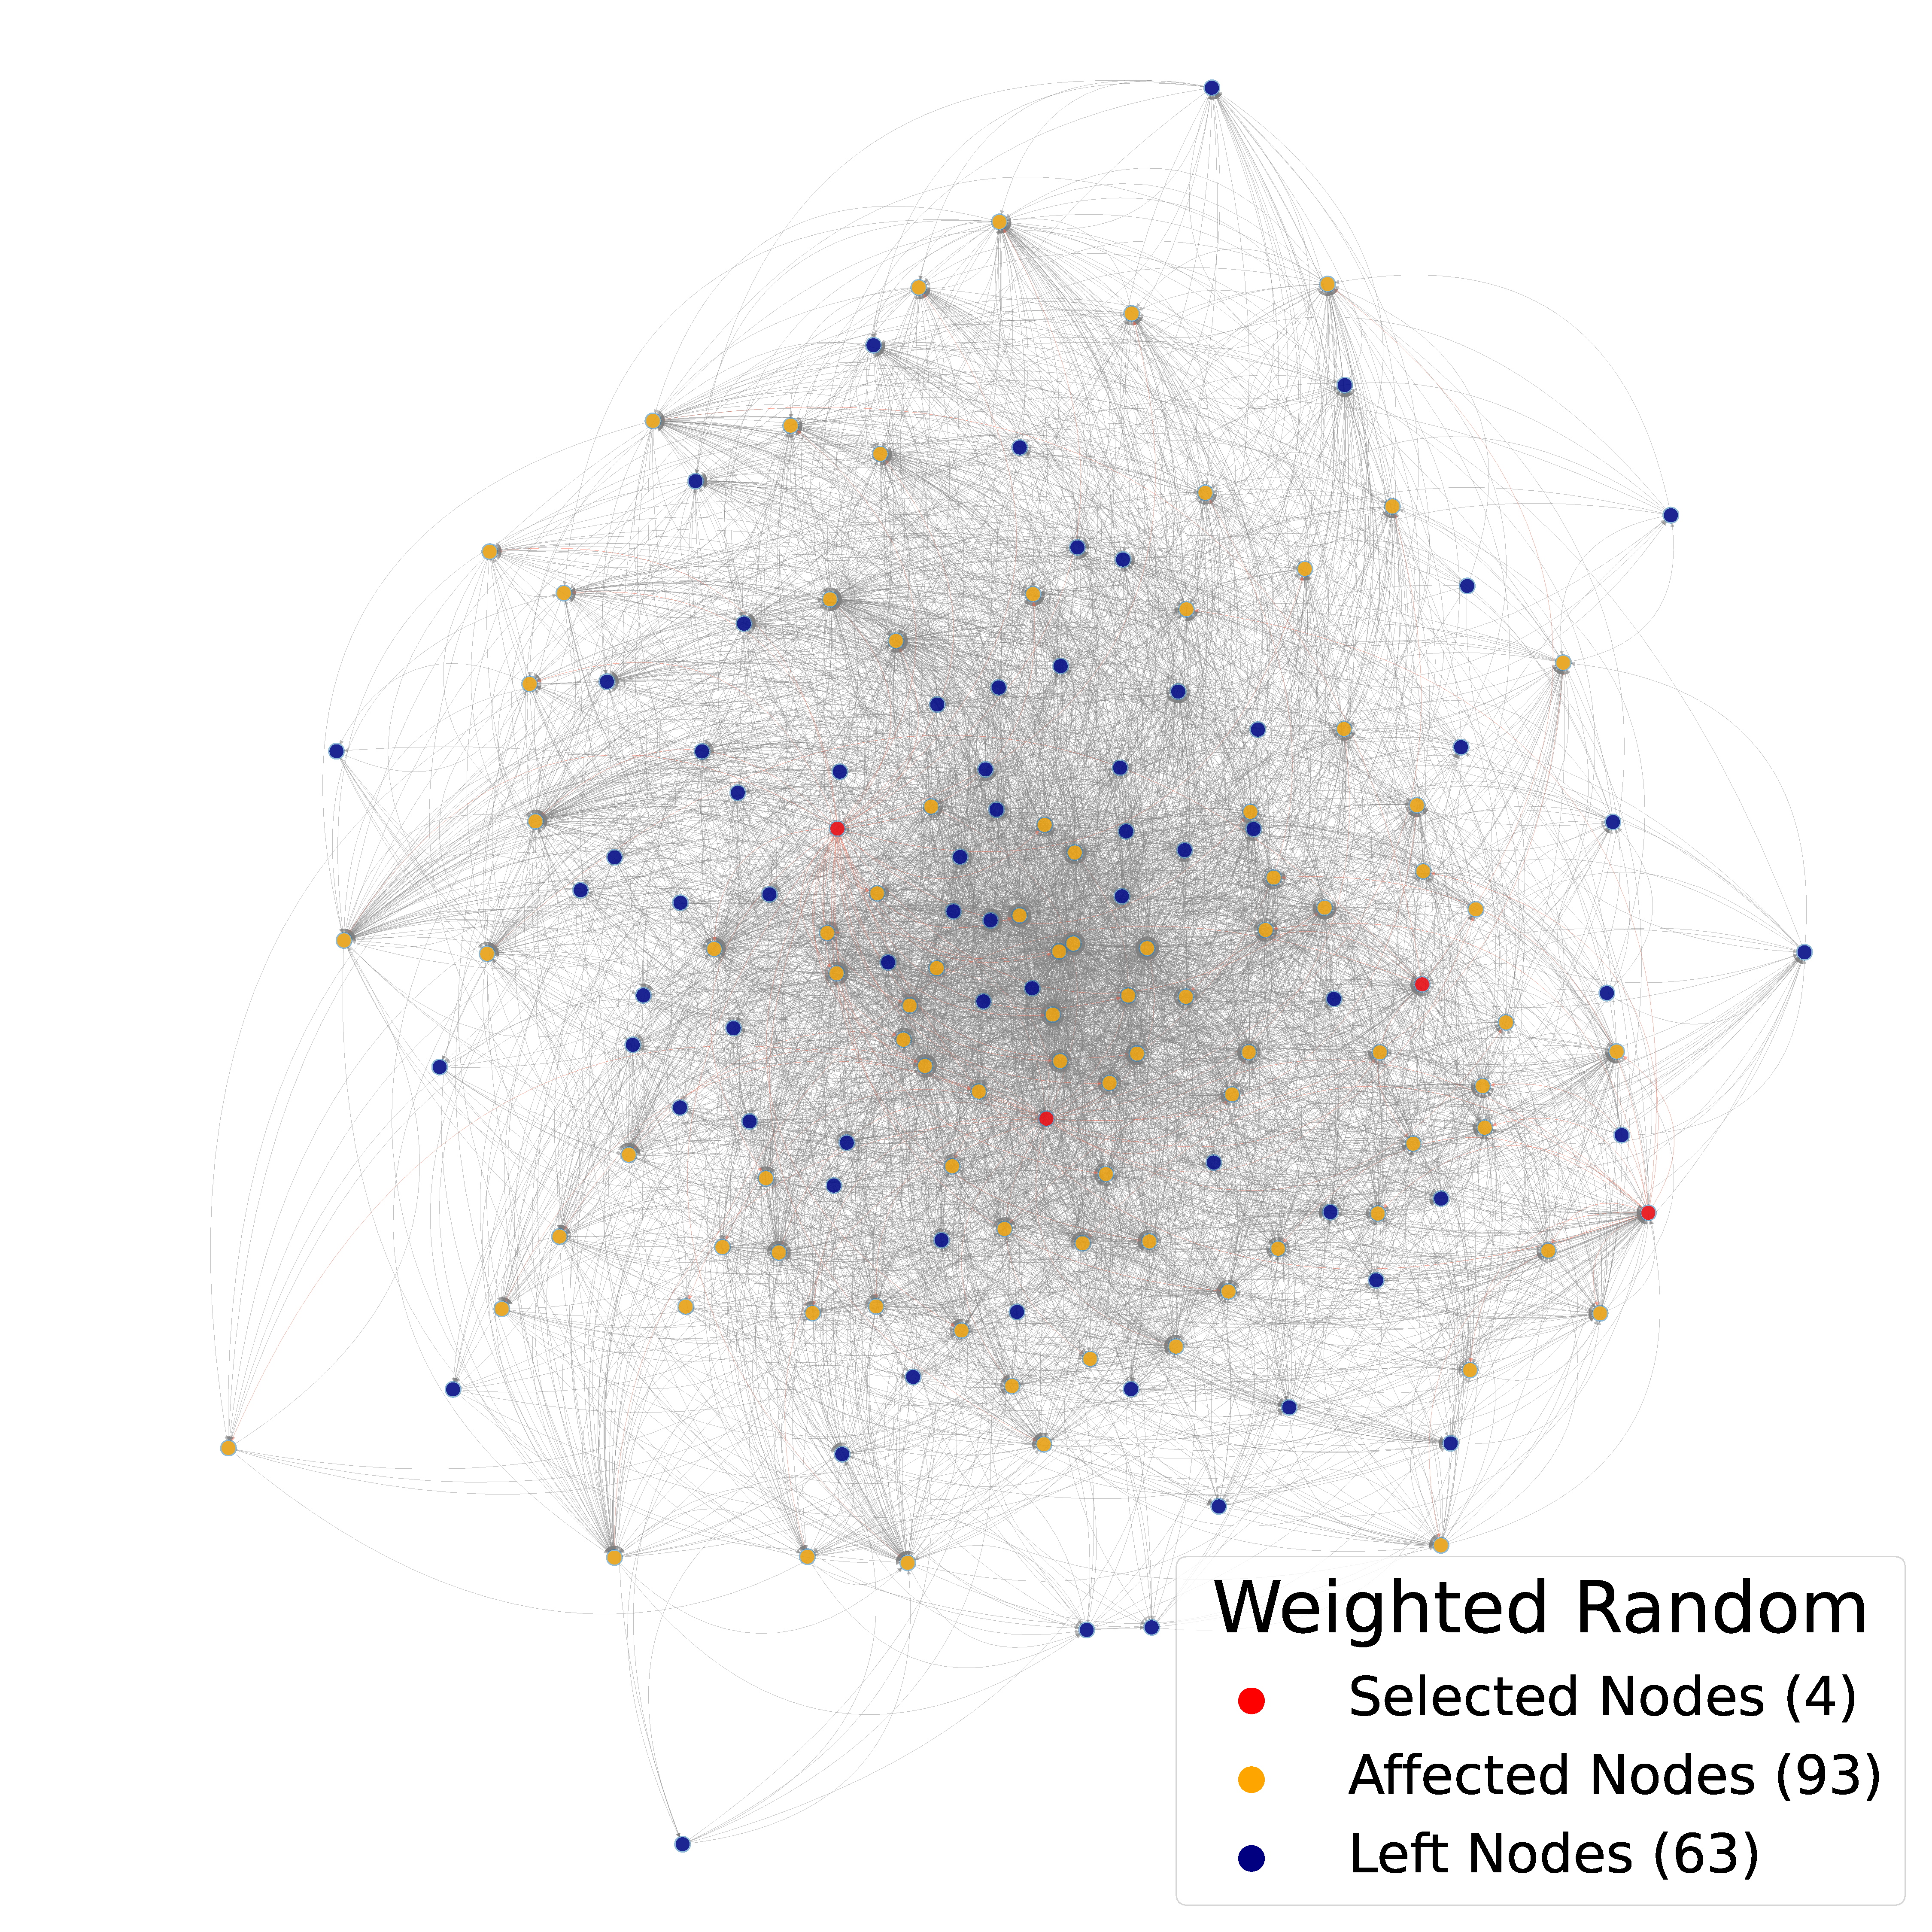
\includegraphics[width=\linewidth]{Figures/GraphExperiment/Network/plot_Weighted Random.pdf}
        %\\{\tiny Weighted Random}
        \label{fig:wr}
    \end{minipage}%\hspace{0.005\textwidth}
    \hfill
        % Fourth figure
    \begin{minipage}{0.18\textwidth}
        \centering
        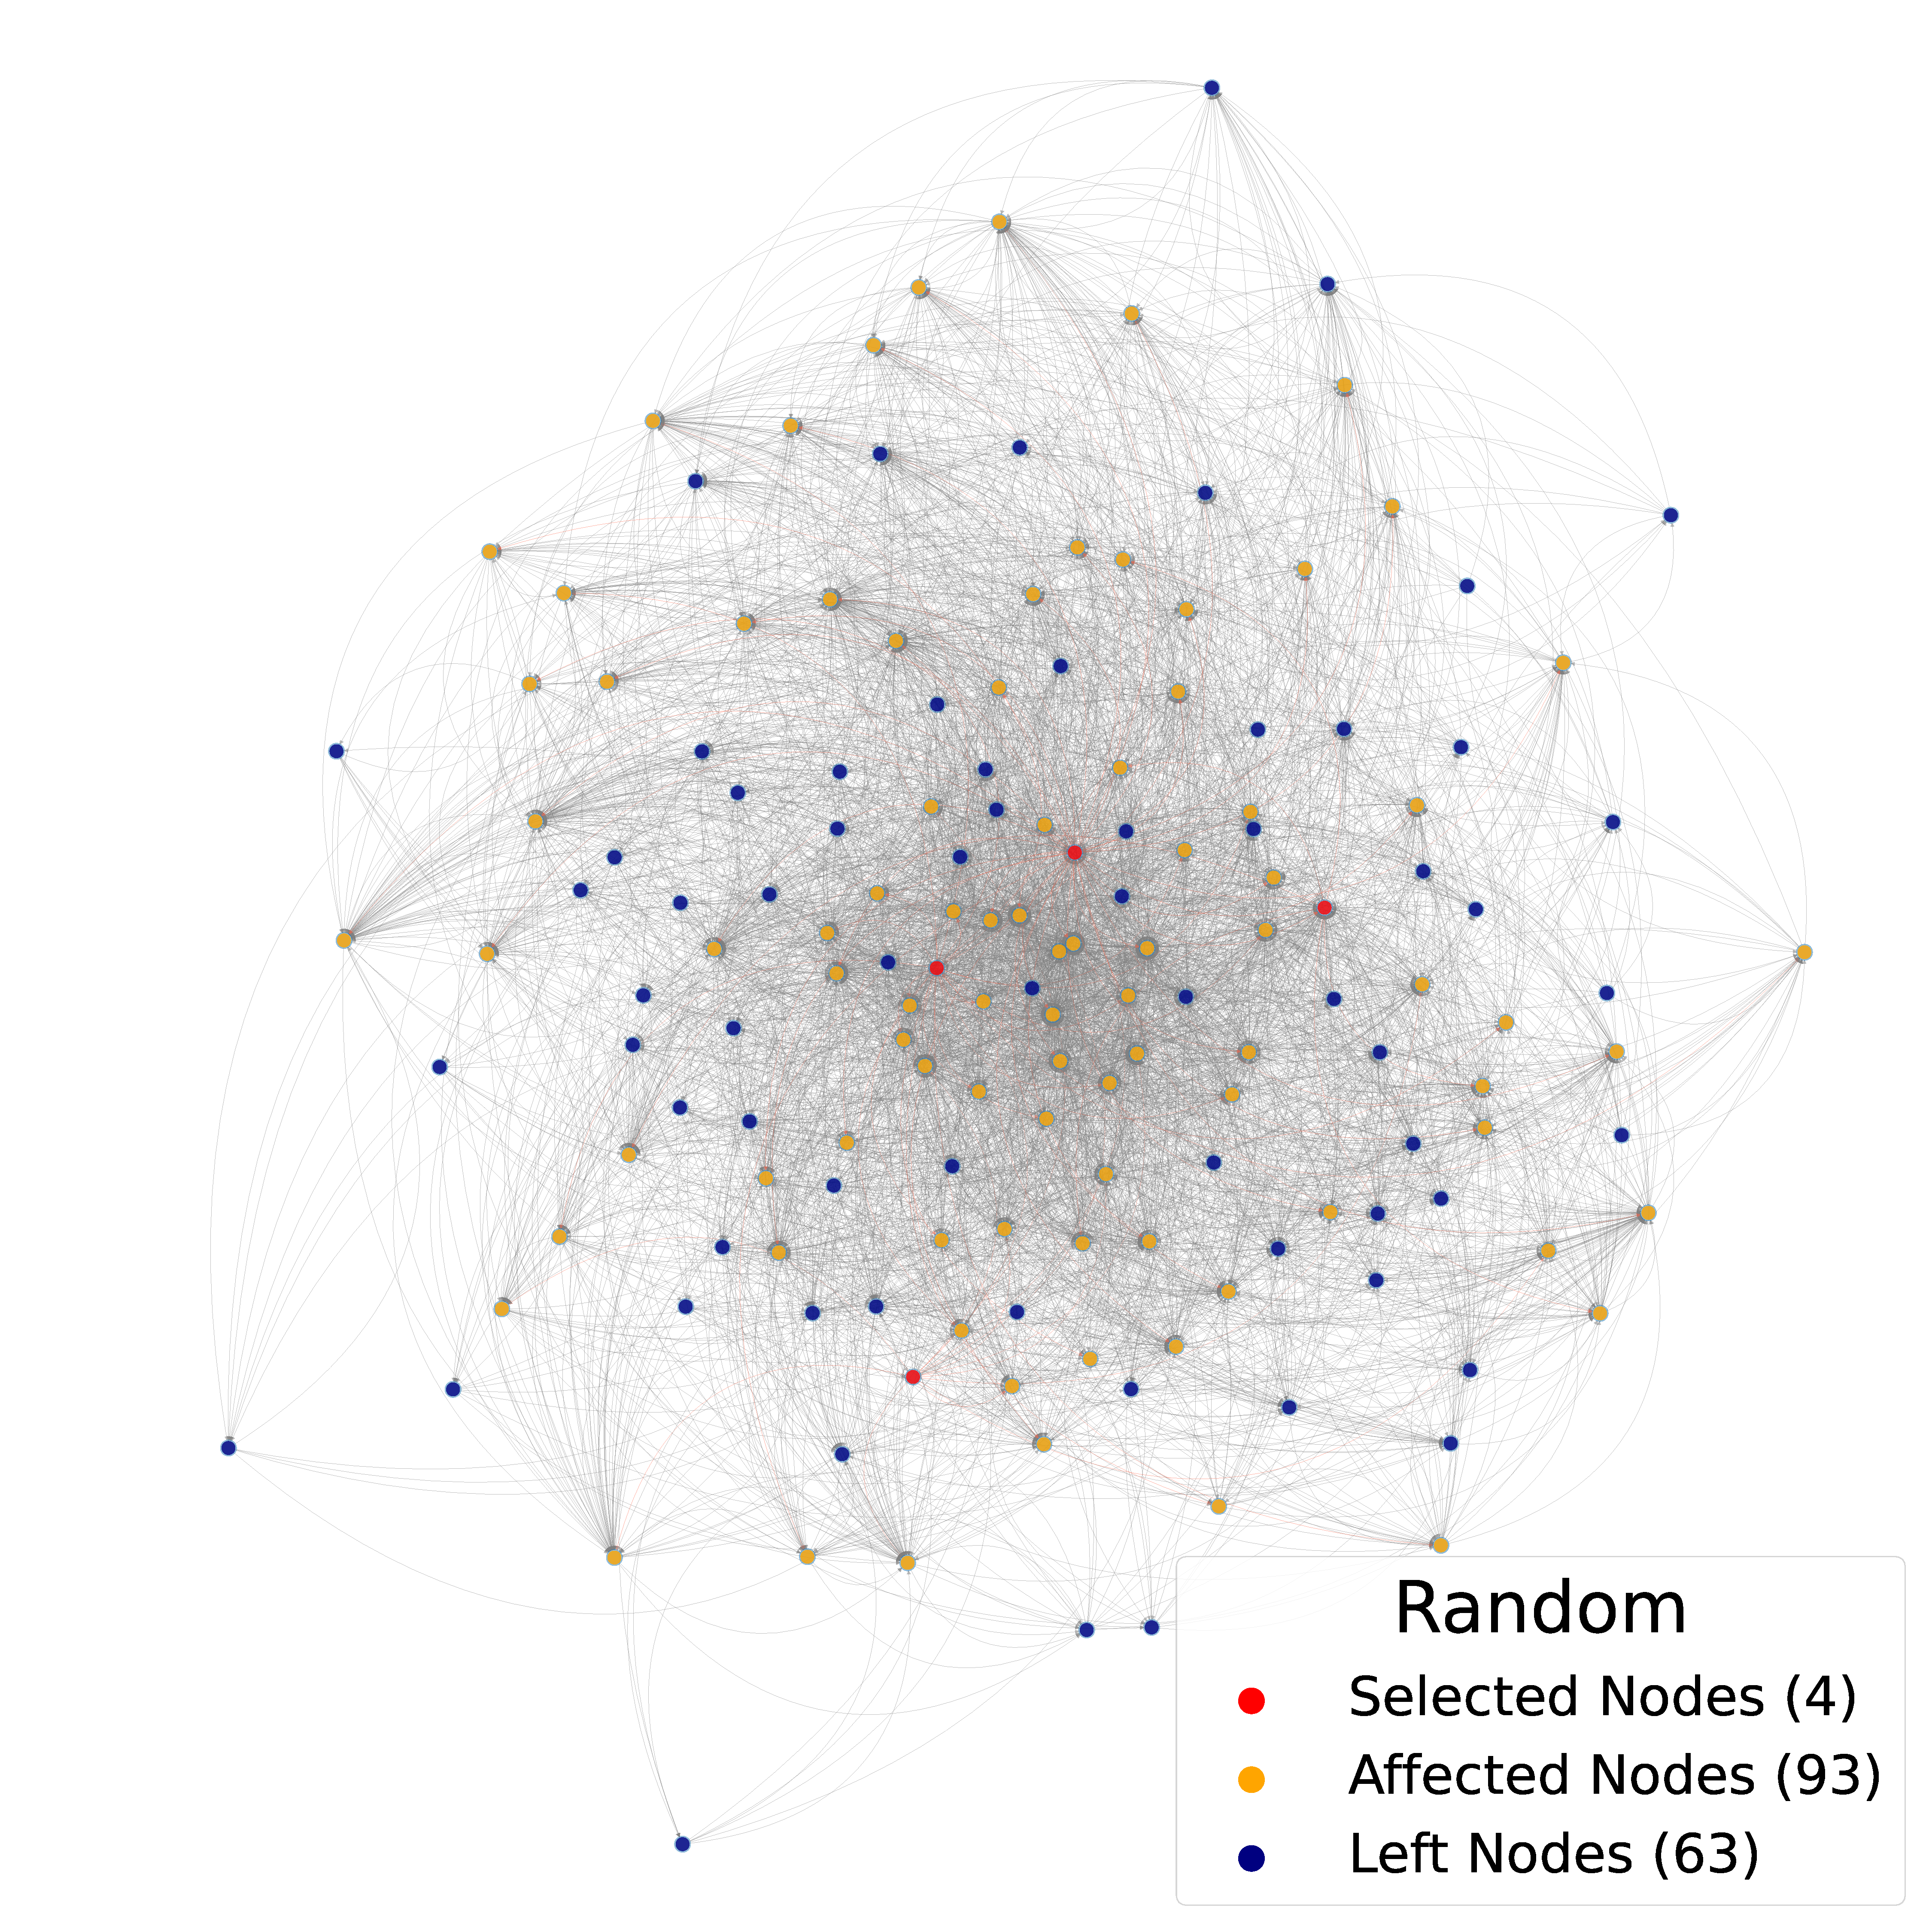
\includegraphics[width=\linewidth]{Figures/GraphExperiment/Network/plot_Random.pdf}
        %\\{\tiny Random}
        \label{fig:random}
    \end{minipage}%\hspace{0.005\textwidth}
    \hfill

    \caption{Node selection on a sub-network of Reddit ($K = 4$ and $\eta=4$). High-degree nodes are displayed in large sizes; selected nodes are marked red with red out-edges linked to affected nodes (orange). The performance decline from left to right.}
    \label{fig:network visualisation}
\end{figure*}


\begin{figure*}[t!]
    \centering
    % First figure
    \begin{minipage}{0.245\textwidth}
        \centering
        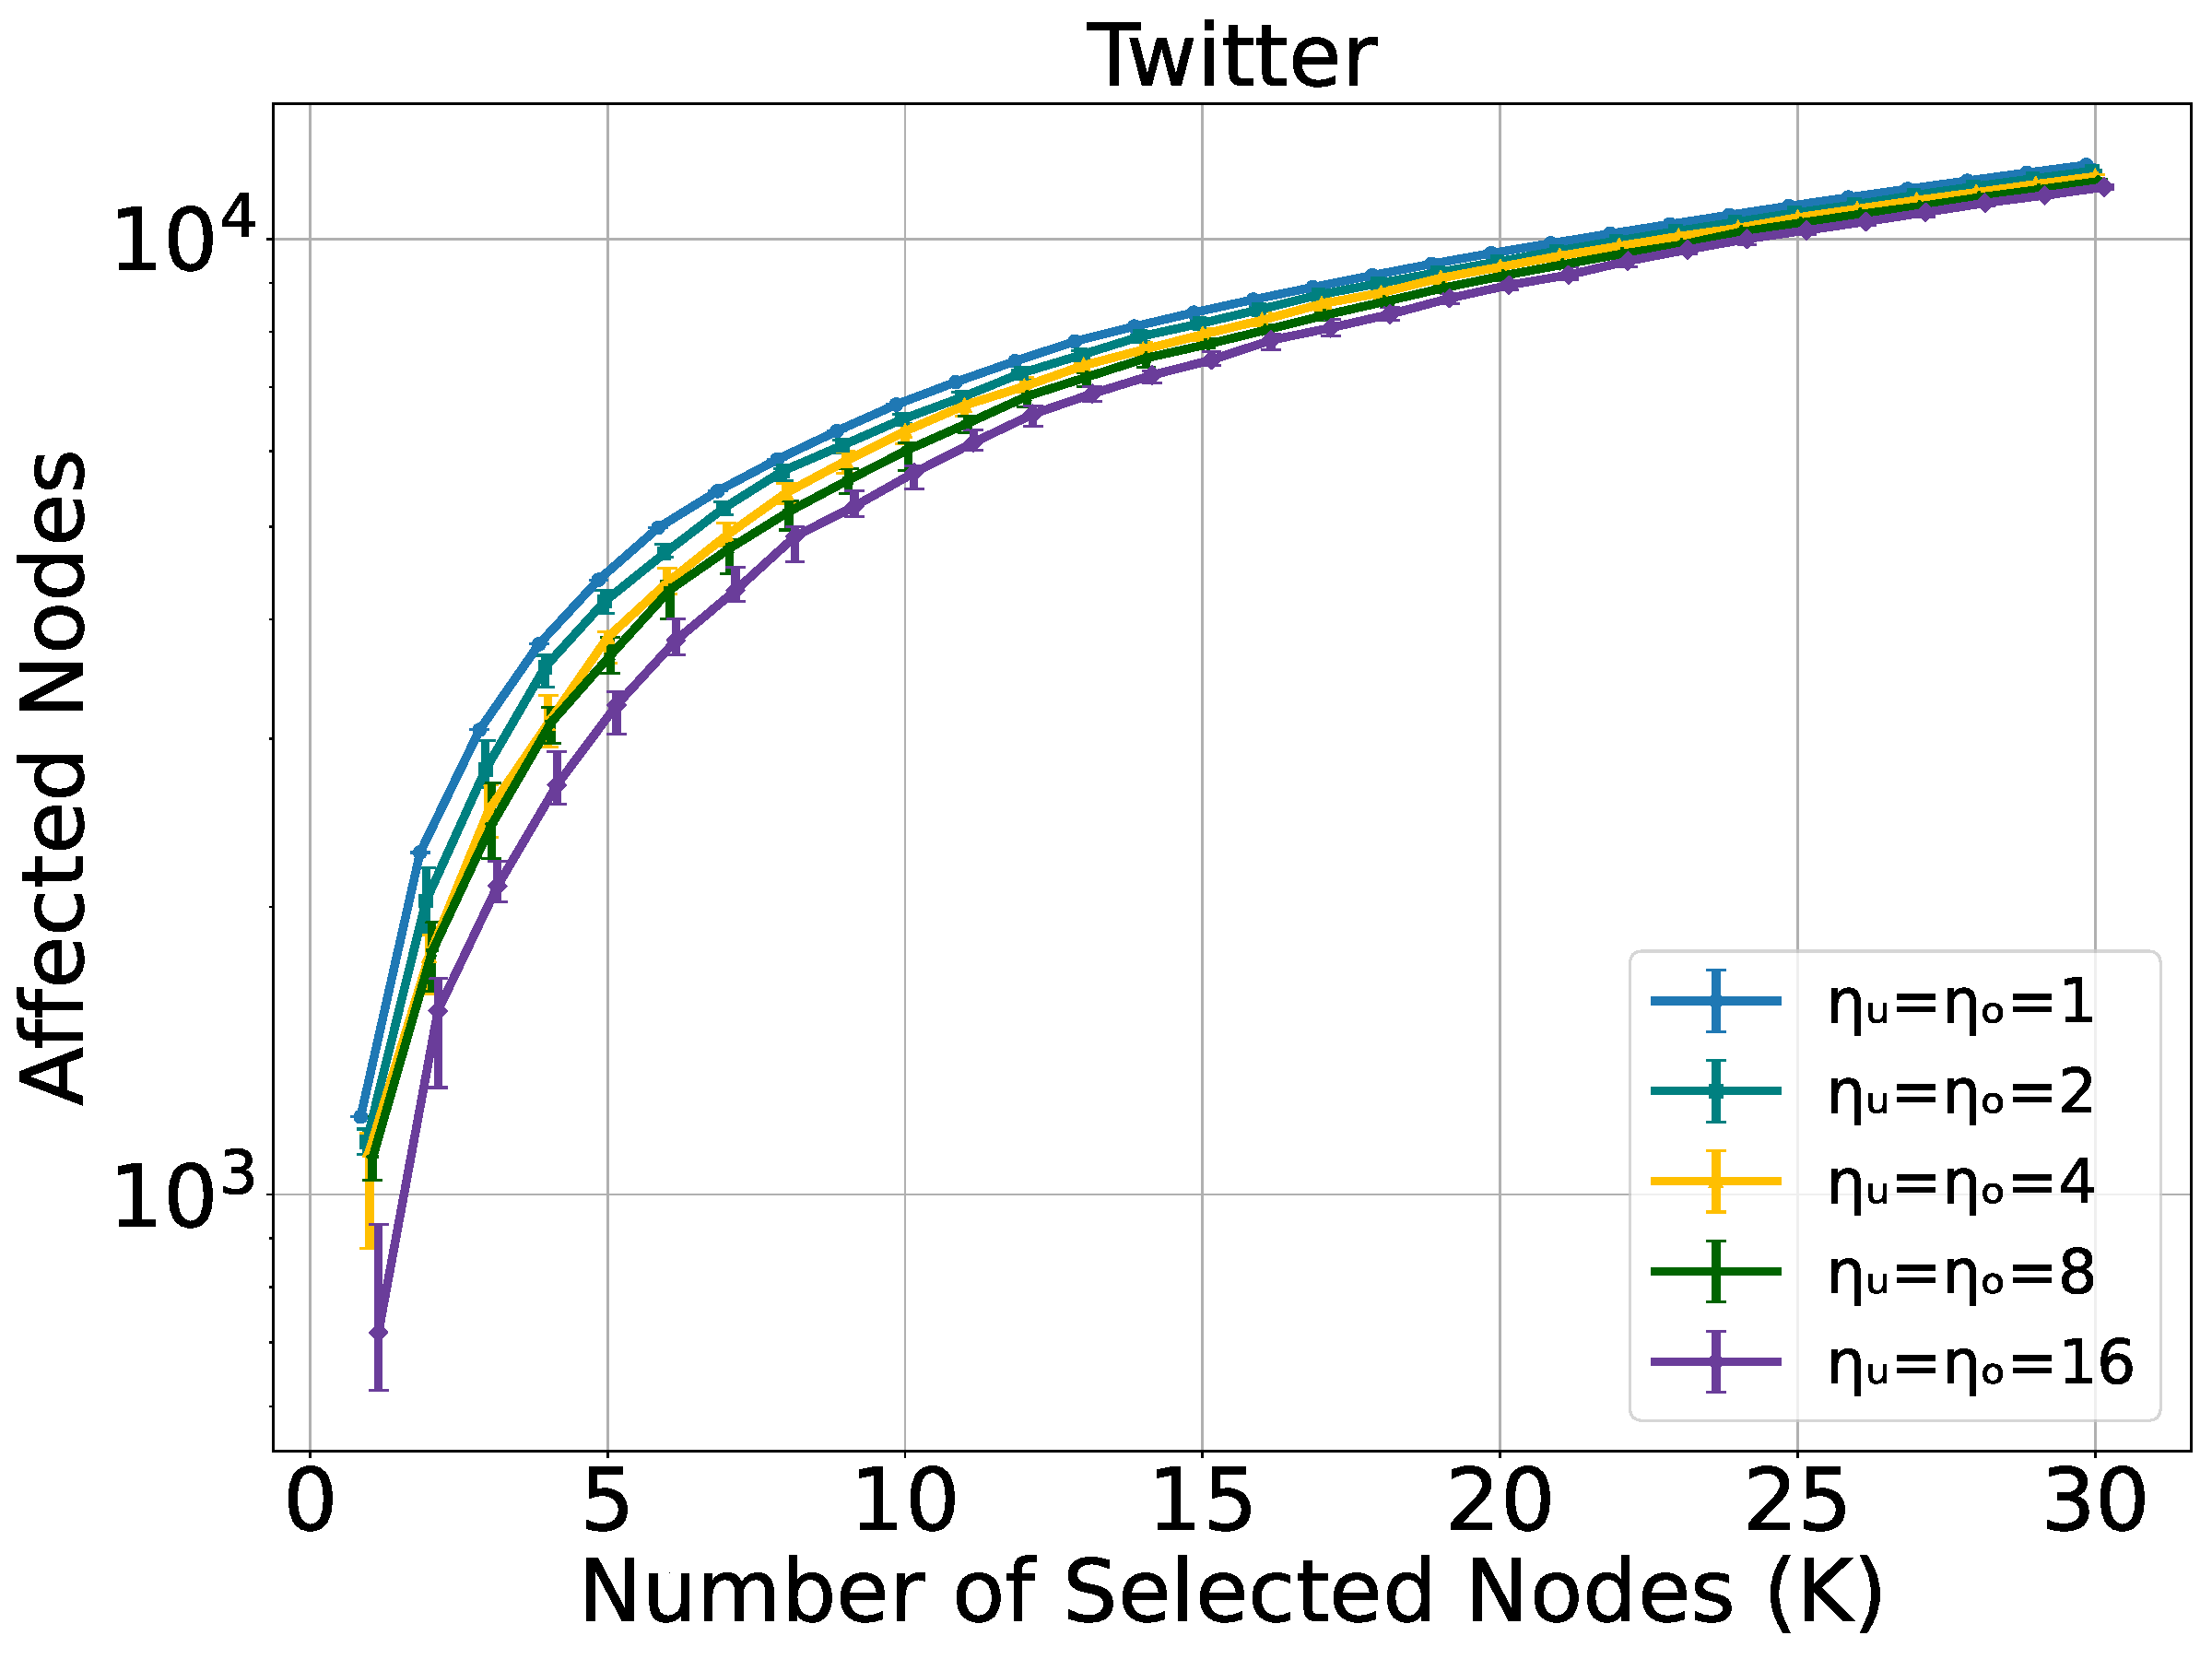
\includegraphics[width=\linewidth]{Figures/GraphExperiment/Errors/new/error_twt.pdf}
        \label{fig:error_twt}
    \end{minipage}\hfill
    % Second figure
    \begin{minipage}{0.245\textwidth}
        \centering
        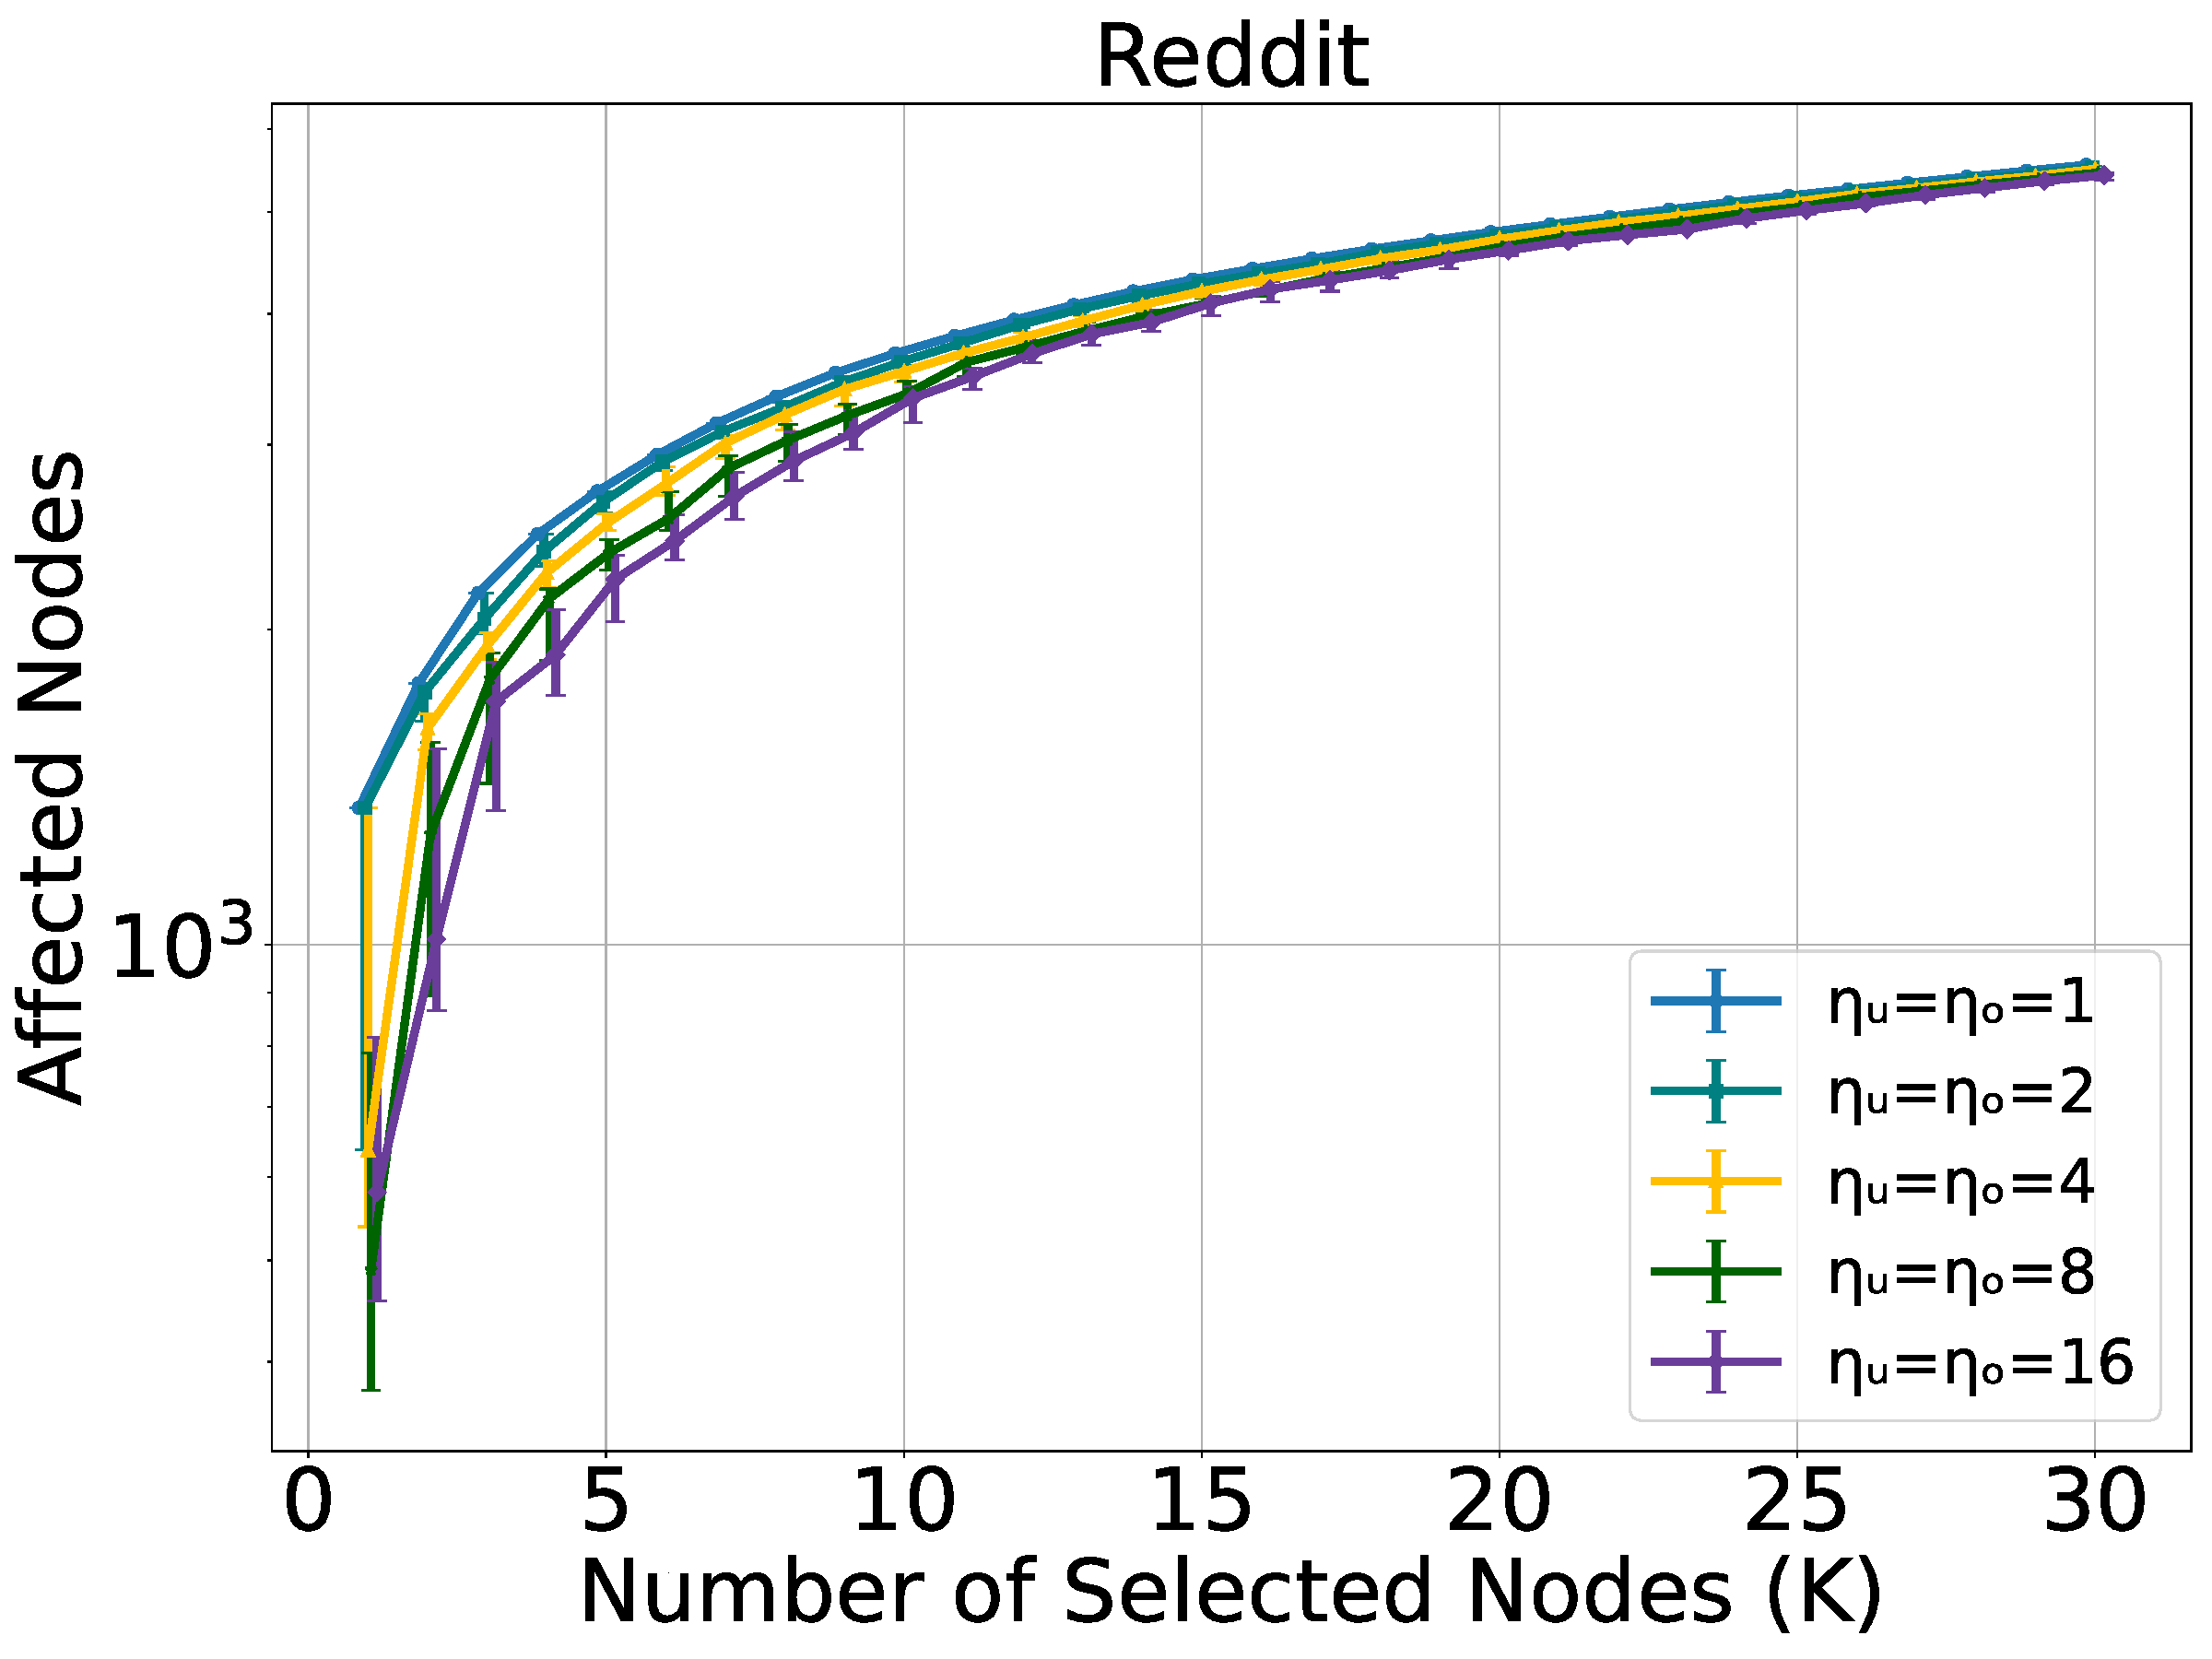
\includegraphics[width=\linewidth]{Figures/GraphExperiment/Errors/new/error_rdt.pdf}
        \label{fig:error_rdt}
    \end{minipage}
    \hfill
    % Third figure
    \begin{minipage}{0.245\textwidth}
        \centering
        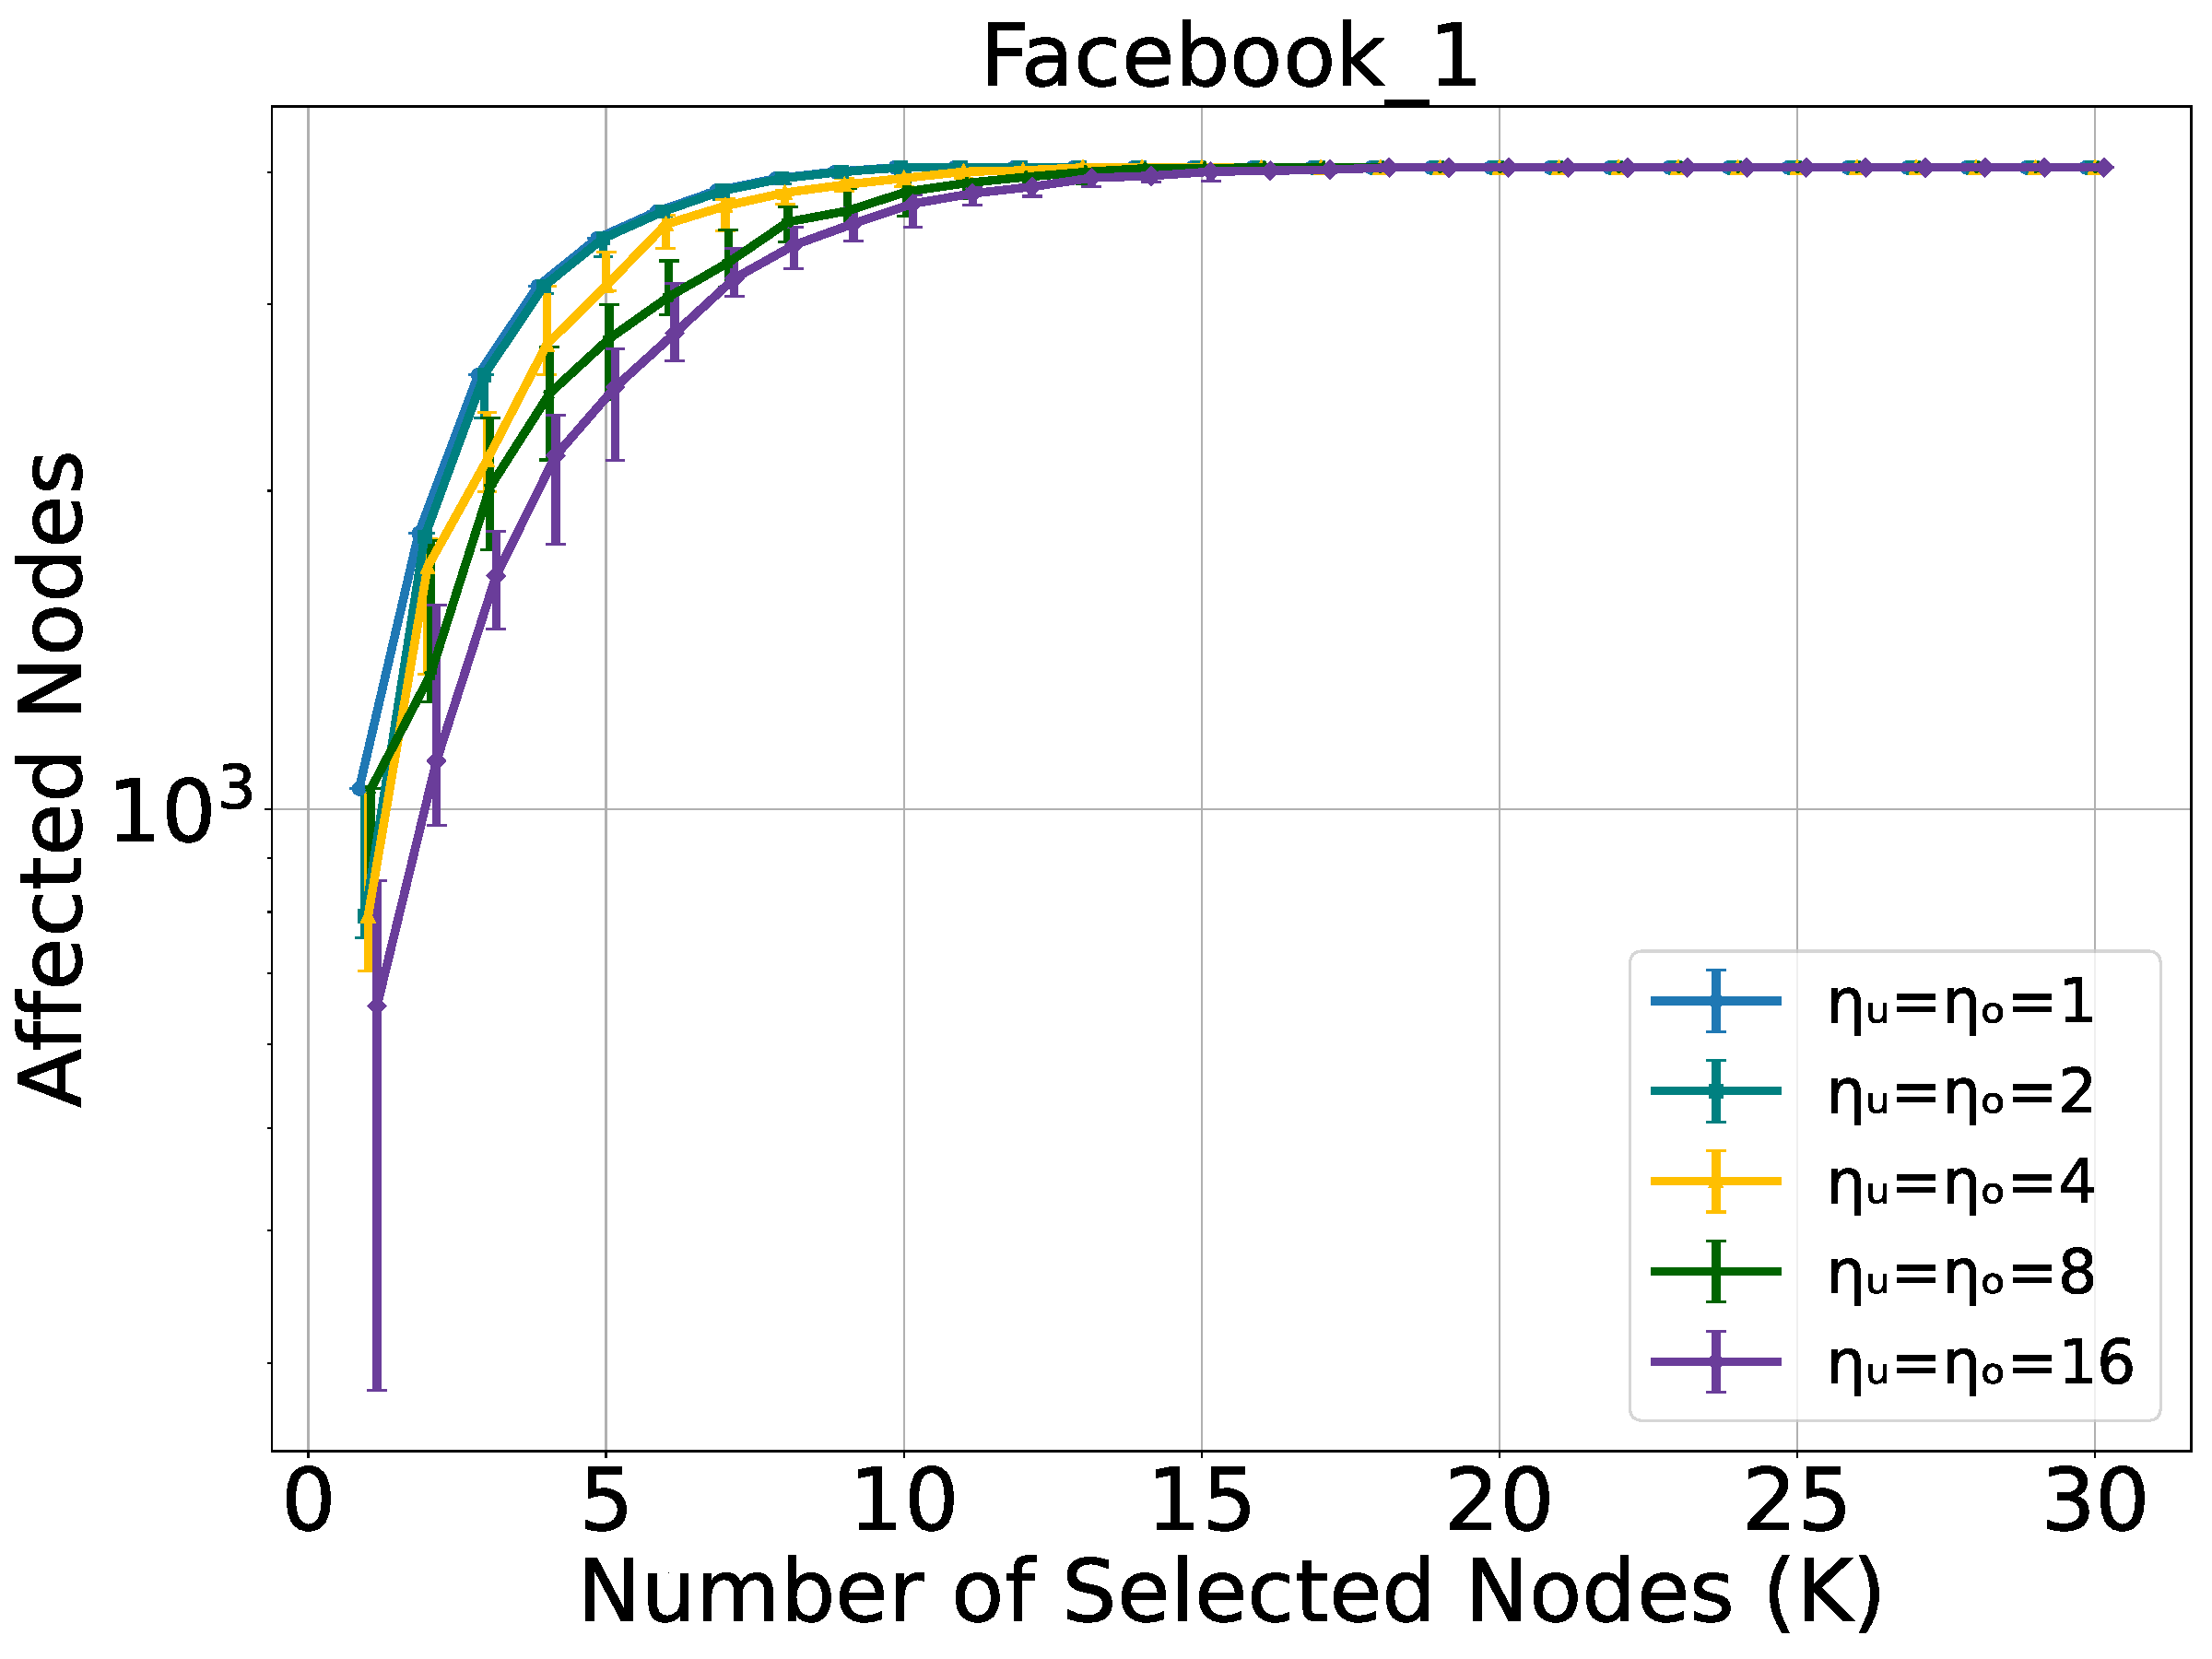
\includegraphics[width=\linewidth]{Figures/GraphExperiment/Errors/new/error_fb1.pdf}
        \label{fig:error_fb1}
    \end{minipage}
    \hfill
    % Fourth figure
    \begin{minipage}{0.245\textwidth}
        \centering
        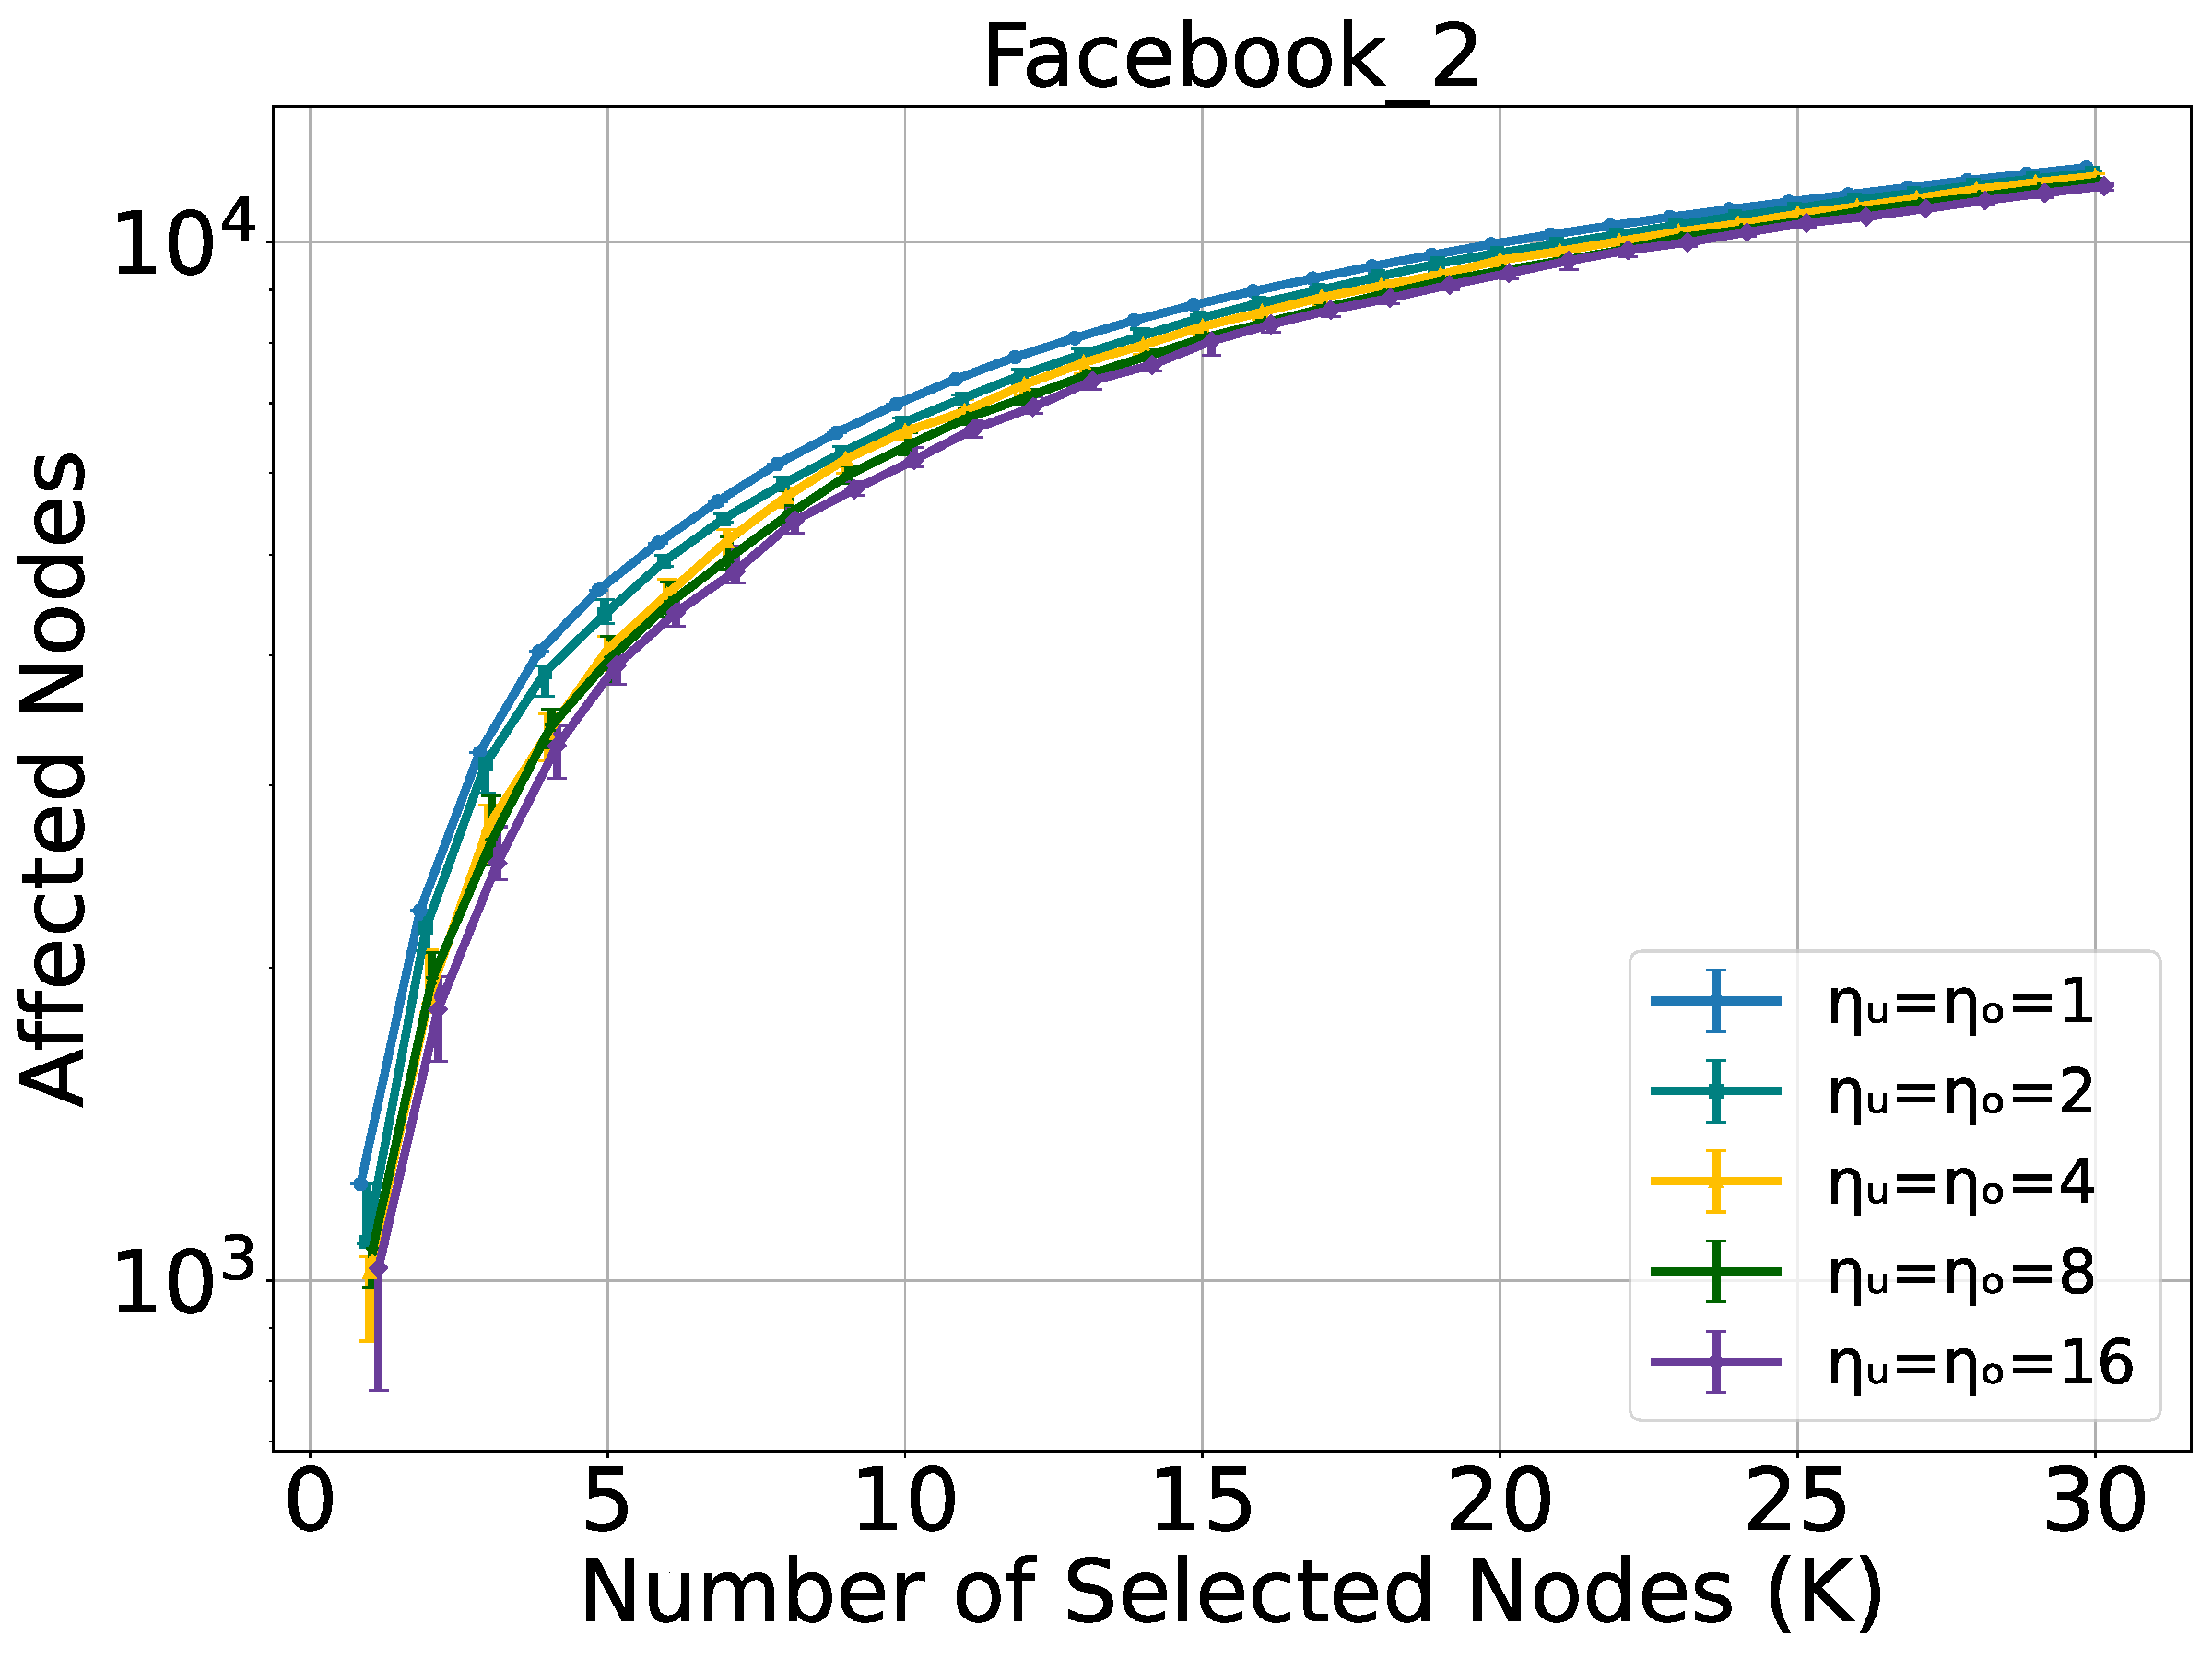
\includegraphics[width=\linewidth]{Figures/GraphExperiment/Errors/new/error_fb2.pdf}
        \label{fig:error_fb2}
    \end{minipage}
    %\vspace*{-5mm}
    
    \caption{Affected nodes with an increasing $K$ by SOP-Greedy with $\eta \in [1, 16]$.}
    \label{fig:graph error}
\end{figure*}

\begin{figure*}[t!]
    \centering
    % First figure
    \begin{minipage}{0.245\textwidth}
        \centering
        
\includegraphics[width=\linewidth]{Figures/experiment 2/new/c2_twt.pdf}
        \label{fig:RSOP_C_twt}
    \end{minipage}\hfill
    % Second figure
    \begin{minipage}{0.245\textwidth}
        \centering
        
\includegraphics[width=\linewidth]{Figures/experiment 2/new/c2_rdt.pdf}
        \label{fig:RSOP_C_rdt}
    \end{minipage}
    \hfill
    % Third figure
    \begin{minipage}{0.245\textwidth}
        \centering
        
\includegraphics[width=\linewidth]{Figures/experiment 2/new/c2_fb1.pdf}
        \label{fig:RSOP_C_fb1}
    \end{minipage}
    \hfill
    % Fourth figure
    \begin{minipage}{0.245\textwidth}
        \centering
        
\includegraphics[width=\linewidth]{Figures/experiment 2/new/c2_fb2.pdf}
        \label{fig:RSOP_C_fb2}
    \end{minipage}

    \caption{Comparisons of SOP-Greedy and RSOP-Greedy with increasing $K$ under various $\eta_u$ and $\eta_o$.
    %\ref{appendix:large-scale}.
    }
    \label{fig:RSOP_C}
\end{figure*}



\textbf{Experimental set-up.} We consider two classification tasks: airline passenger satisfaction classification \cite{jiang2022forecast} and breast cancer detection \cite{assegie2021breast}. The benchmarks are \textit{SelectKBest} \cite{otchere2022application}, \textit{Recursive Feature Elimination (RFE)} \cite{sachdeva2022systematic}, \textit{Mutual Information} \cite{feature-selection}, and \textit{Extra Trees} \cite{extra-trees}. %Descriptions of data and benchmarks are in Appendix D. %\ref{appendix:descriptions-data-benchmarks}. 
Both tasks have the following set-up. 
Data are randomly split into training data (80\%) and oos data (20\%). The model $h$ is decision tree with the default hyper-parameters and fitting procedure of \textit{scikit-learn}. 
Function $\mathcal{L}$ is the oos accuracy. 
The cardinality constraint $K$ varies from $1$ to $7$. 
%, due to the initial observation that further increasing $K$ does not change accuracy. 
The predictor $\tilde{f}$ is an \textit{independent erroneous oracle}: querying $d_B(A)$ returns $d_B(A) \cdot \text{exp}(X)$ with $X \sim \mathcal{U}(-\log \eta_u, \log \eta_o)$, where $\eta = \eta_u \cdot \eta_o \in [1, 400]$. We know that sampling can exploit independent errors to achieve vanishing errors \cite{submodularOptNoisetoImageCollection}. However, in our implementation, value $d_B(A)$ is queried at most once for any $A, B \subseteq [n]$, making errors effectively \textit{consistent}. 
We implement the R-step predictive greedy ($R = 1, 2, 3$), which we call SOP-Greedy (Submodular Optimization Predictive Greedy). %, with implementation details. %\ref{appendix:experiment1-implementations} 
We run the predictive greedy 30 times and report InterQuartile Range (IQR) of the results to take the randomized error generation into account. We also compute a lower bound for the empirical performance ratio of SOP-Greedy defined as $\frac{f(S_{\text{SOP}})}{\mathrm{OPT}}$, where $S_{\text{SOP}}$ denotes the solution returned by SOP-Greedy and OPT the optimal value. We set $\text{OPT} = 1$ to under-estimate the true ratios. The experiments are conducted with processor Intel Core 12600KF, RAM 16GB, and GPU Nvidia Geforce RTX 3070, 8GB VRAM. 

% Present the results; discuss observtions and implications

\textbf{Results.} Figure \ref{fig:experiment1-performance} presents the oos accuracy for different algorithms on two datasets with varying $K$ and $\eta$. The accuracy under an increasing $K$ is approximately increasing and concave, reflecting diminishing gains. 
%\textcolor{red}{it shows the consistency between the submodular function and SOP-Greedy.} 
SOP-Greedy can access $\tilde{f}$, but the other benchmarks can use $\boldsymbol{X}$ and $y$ to measure in-sample correlations between features and targets. The results show that SOP-Greedy consistently outperforms the benchmarks for $K > 1$. One may argue that the superiority may be attributed to the informational advantage of knowing the (erroneous) oos performance. However, the algorithm maintains robust performance even with unreasonably large errors (up to $400$), i.e., the errors merely affect performance. This suggests that predicting the exact oos performance might be less critical than the ordering of the oos performance for different feature sets. It shows that (1) the OOS performance forecasts are solid indicators for feature selection, even if they might be far from accurate, and (2) robustness of SOP-Greedy under bad predictions. The performance downgrades gracefully with increasing prediction errors, as shown in the last two figures, showing the smoothness of SOP-Greedy. 
%showcasing its substantial robustness by remaining successful even under worst-case prediction errors. 
%The smoothness is validated by changing the error values because the algorithm's performance is consistent across different prediction qualities.


Figure \ref{fig:experiment2-R-step} presents the oos accuracy of the R-step predictive greedy (RSOP-Greedy) with varying $R$. The algorithm observes slight improvements with an increased $R$. Still, the improvements are insignificant, although the theoretical worst-case bounds are improved. We suspect this might be because the errors are not adversarial, so the benefit of searching a larger space is marginal. The estimated empirical performance ratios of SOP-Greedy against the theoretical bounds are shown in Tables \ref{tab:airline-r-steps-theo} and \ref{tab:breast-r-steps-theo}. The empirical performance ratios well-exceed the theoretical bounds derived previously. This suggests that our theoretical bounds are pessimistic even if we assume OPT is 1, showing that the algorithm performs comparably to the optimum in practice. 






%The results constantly demonstrate that this methodology outperforms the results of the four benchmark methodologies: the approach's higher performance is primarily attributed to its dynamic gain computation, which is distinguished from the other four techniques. 

%It is noted that as the value of \( K \) grows to a certain threshold, the gains obtained by incorporating additional features start to reduce. After reaching this stage, the accuracy stabilizes and remains nearly constant. 

%The slowing down effect suggests that the predictive power of including additional features decreases once the model has already caught the most important features. This observation is aligned with the properties of submodular functions.

%Besides, our study investigates the impact of changing the error boundaries (\( \eta_u, \eta_o \)) on accuracy across different feature counts \( K \). When the error boundaries (\( \eta_u, \eta_o \)) are reduced, the precision of the feature subsets increases, which could be oberserved in Figure 1 (c) and (d). The above behavior is consistent with the expectation that a more accurate calculation of gains results in an improved selection of features and, therefore, superior performance of the model.






\subsection{Influence maximization} \label{subsec:influence-maximization}


The influence maximization problem models applications like a company targeting individuals in a social network to maximize their influence in a viral marketing campaign under some budget constraint \cite {kempe2003maximizing, bogunovic2017robust, banihashem2023dynamic}. Given a network $G = (V, E)$, our task is to find nodes $S \subseteq V, |S| \leq K$, with the maximum affected nodes. The problem can be cast as the following optimization. 
\[ \max_{S \subseteq V} \{f(S) : |S| \leq K \} \]
where $f(S) := |\{ v| v \in V - S, u \in S, (u, v) \in E \}$. 
The function $f$ is submodular for any graph \cite{mossel2010submodularity}. Our formulation is a special case of \cite{kempe2003maximizing}. The node set $V$ is visible, but the edge set $E$ is not. In the context of a viral marketing campaign, it means the company knows individuals but not links in between. However, the company may use individuals' public information, e.g., followers on social media, as features to build a model as the predictor $\tilde{f}$. We assume a predictor $\tilde{f}$ for $f$ is accessible. 


\textbf{Experimental set-up.} We consider Twitter \cite{facebook&twitter}, Reddit \cite{reddit}, and Facebook \cite{facebook2} networks. We implement \textit{Greedy} (single-step with complete knowledge of $G$), \textit{SOP-Greedy} (predictive greedy with $R=1$), \textit{RSOP-Greedy} ($R=2$), \textit{Weighted Random}, and \textit{Random}, with implementation details in Appendix E. %\ref{appendix:experiment2-implementation-details} 
The predictor $\tilde{f}$ is an independent erroneous oracle: querying $d_B(A)$ returns $d_B(A) \cdot \text{exp}(X)$ with $X \sim \mathcal{U}(-\log \eta_u, \log \eta_o)$. We run the predictive greedy 30 times and report IQR of the outcomes. The experiments are conducted on Intel Core 14700KF with 64GB of RAM. 



% \begin{figure}[ht!]
%     \centering
%     % First row
%     \begin{minipage}{0.48\columnwidth}
%         \centering
%         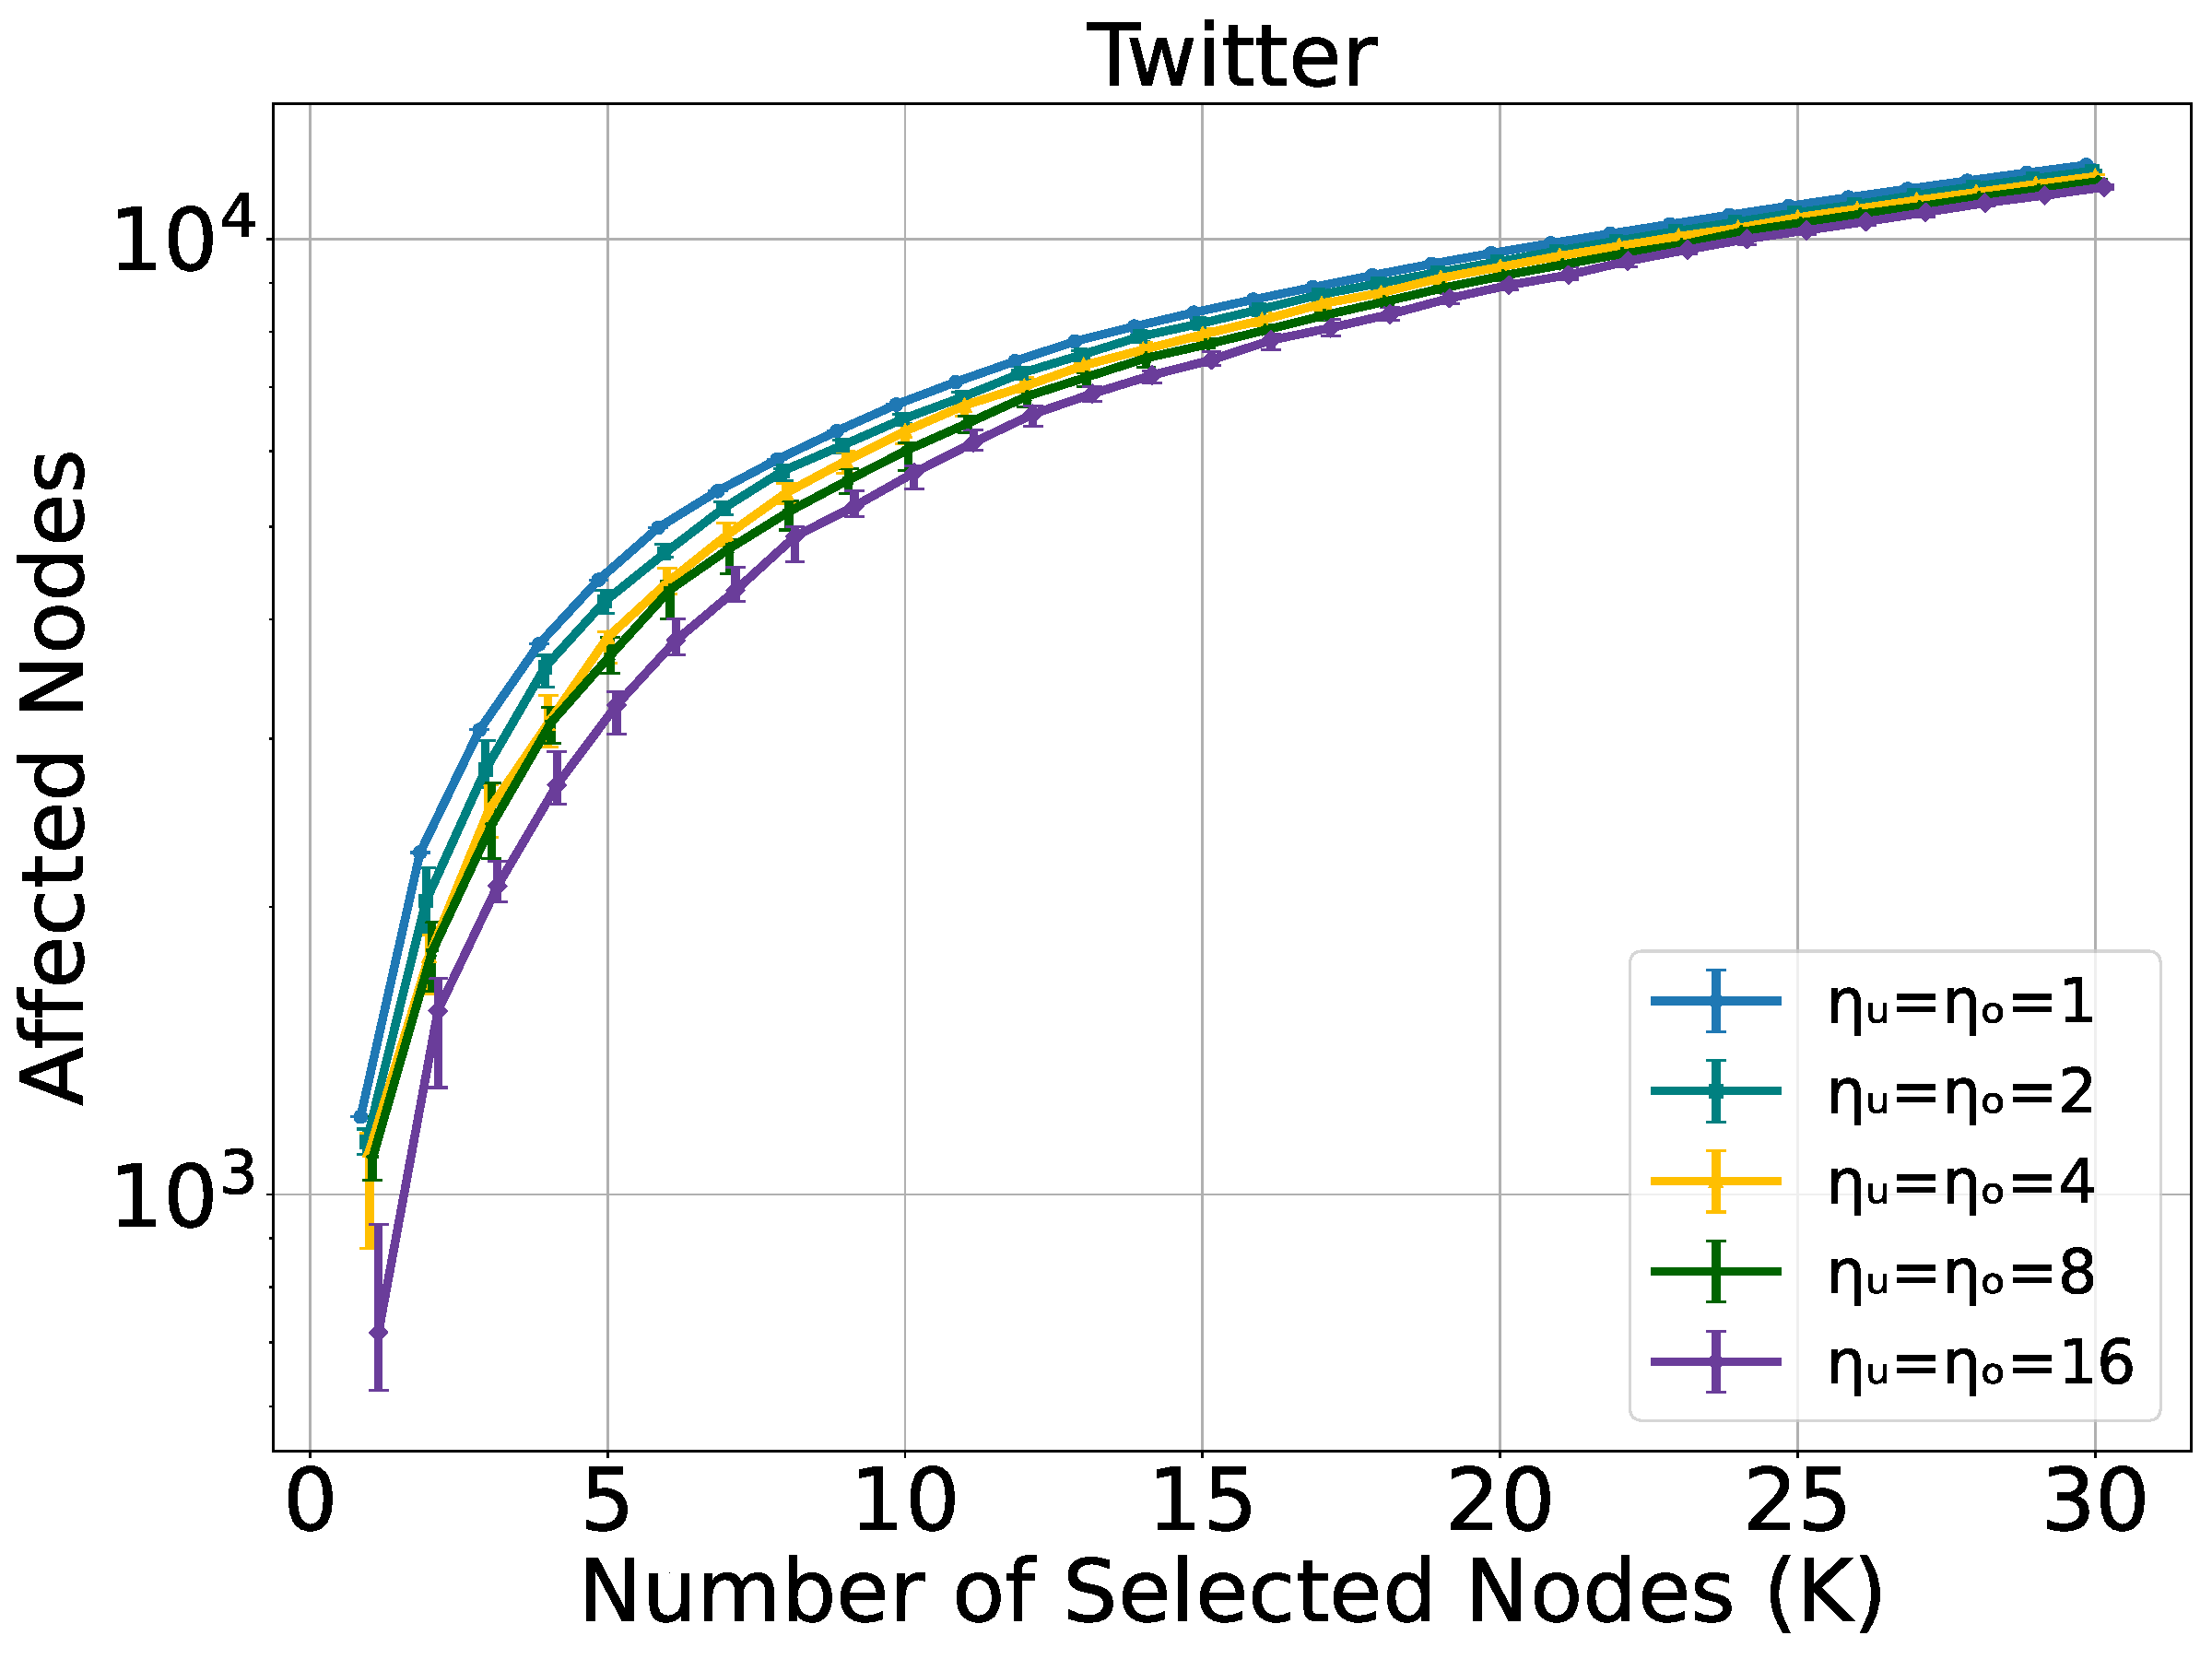
\includegraphics[width=\linewidth]{Figures/GraphExperiment/Errors/new/error_twt.pdf}
%         \label{fig:error_twt}
%     \end{minipage}\hfill
%     \begin{minipage}{0.48\columnwidth}
%         \centering
%         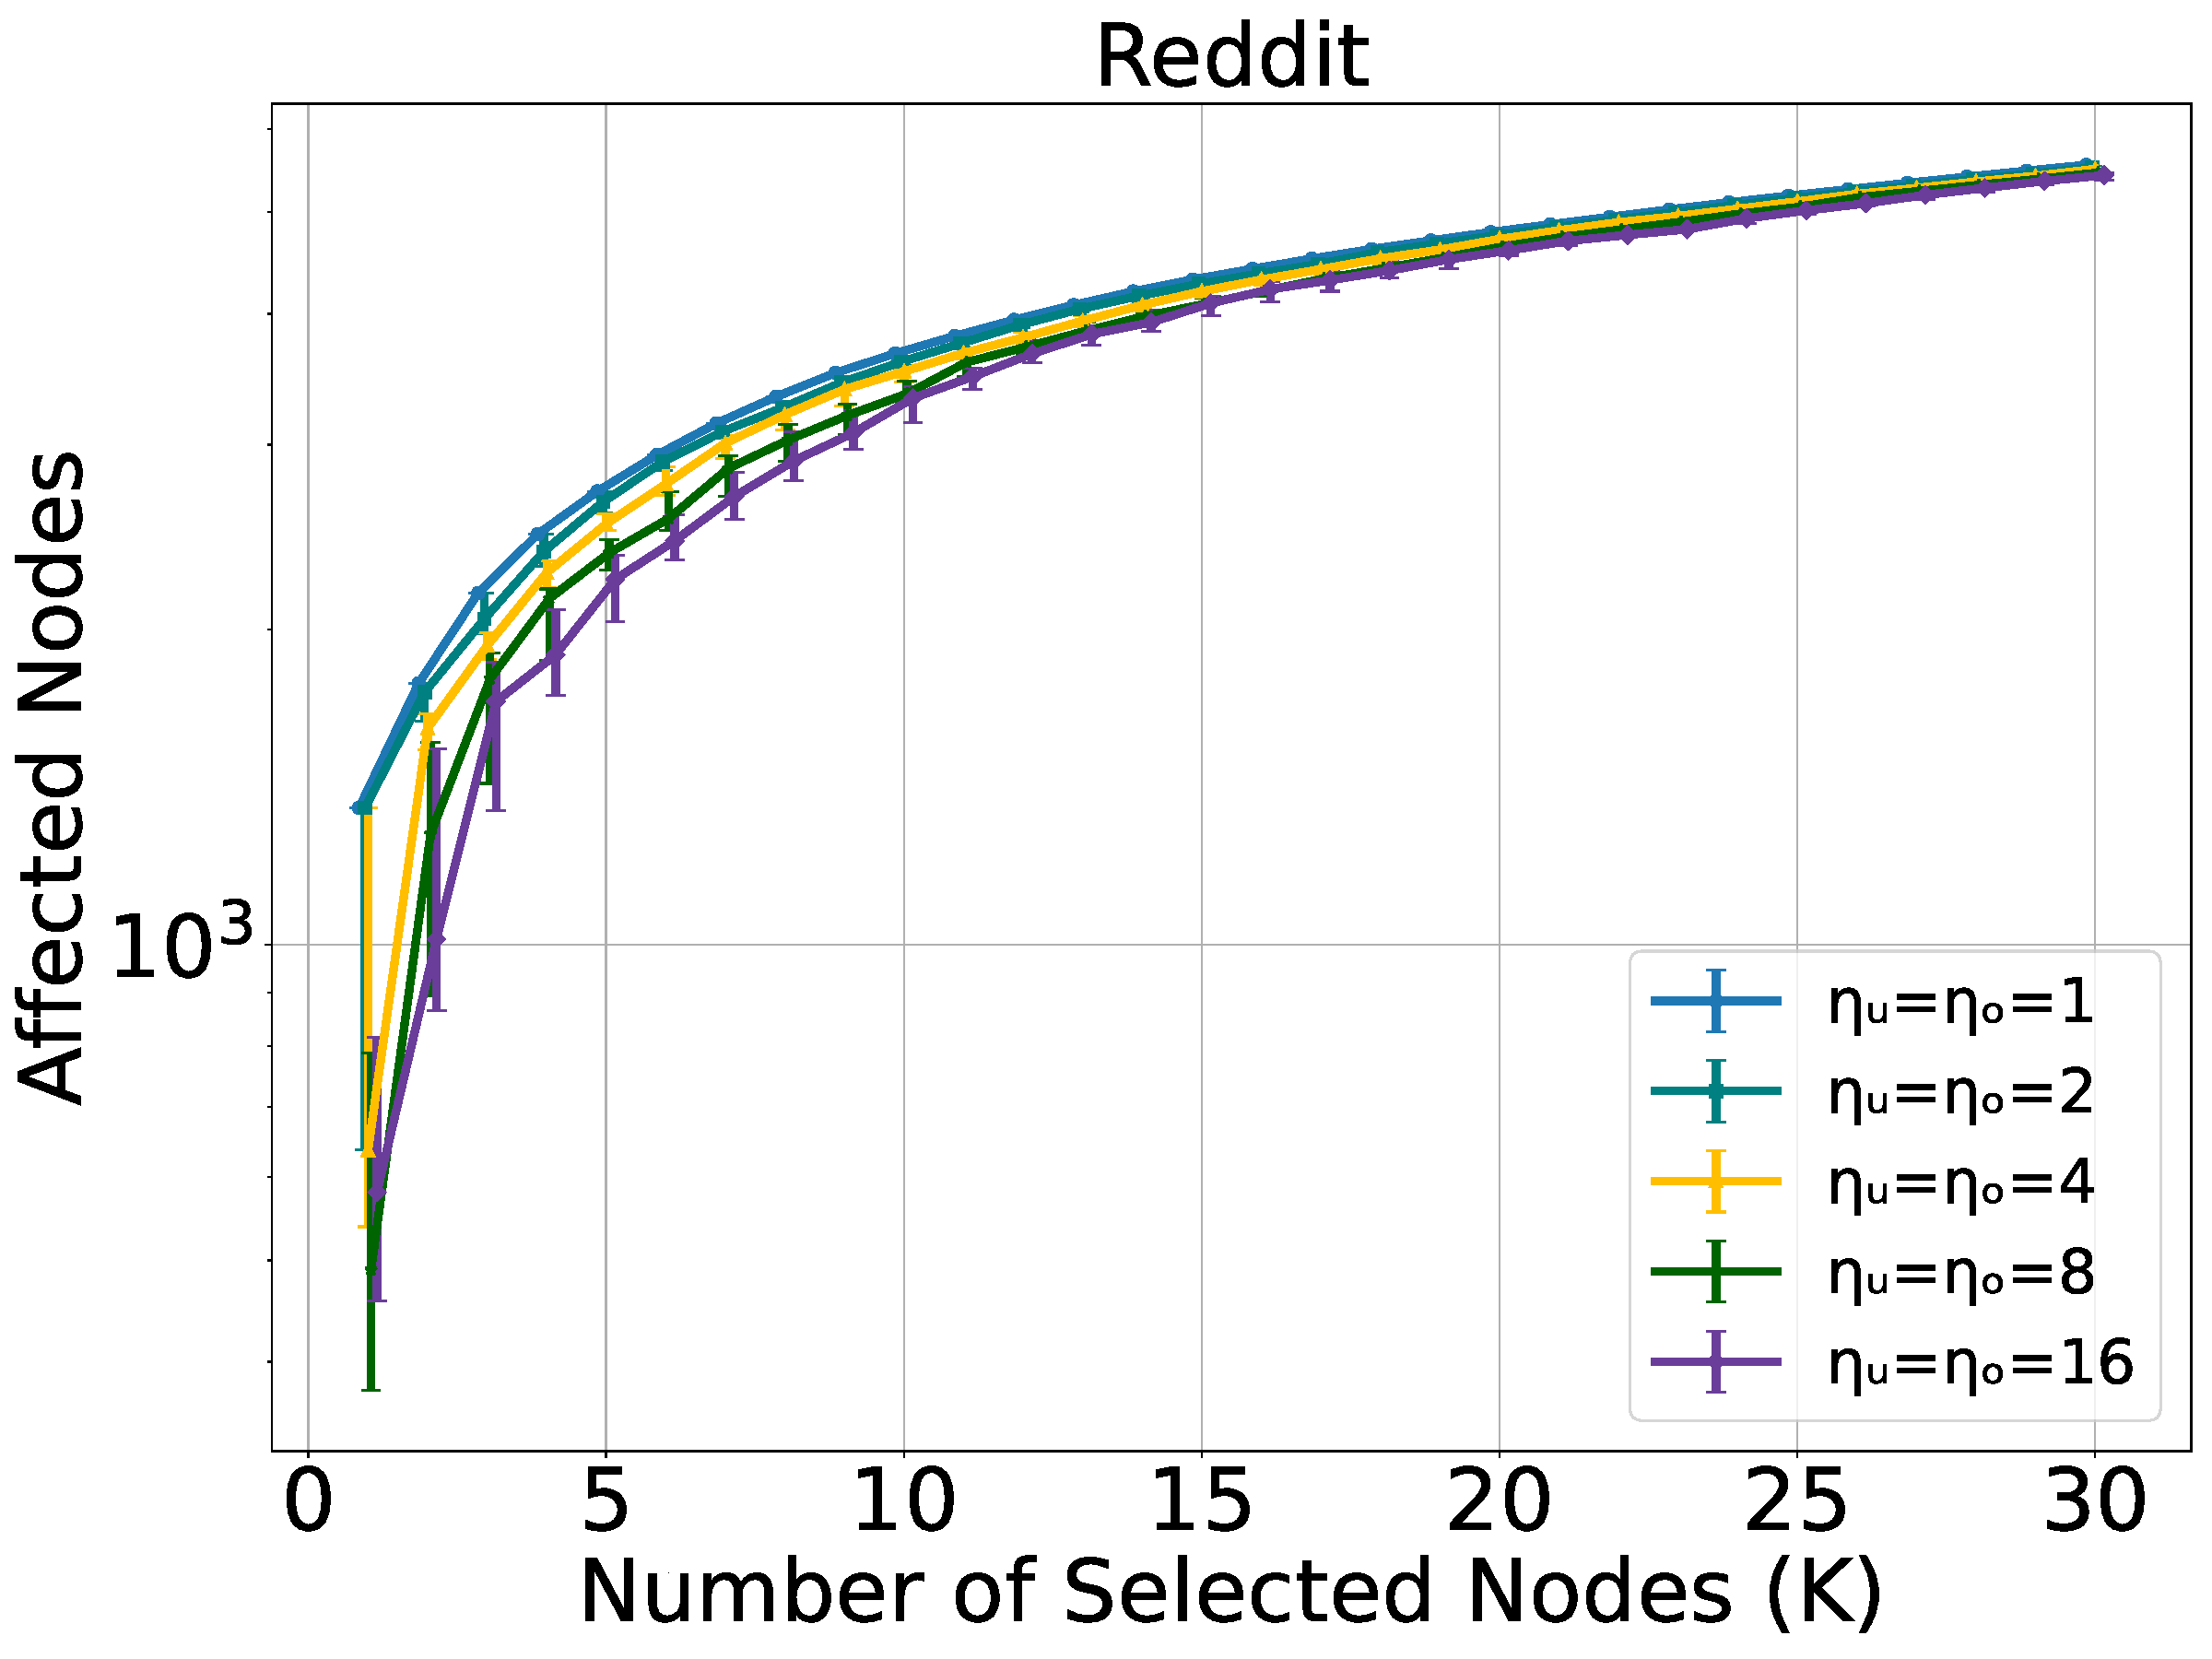
\includegraphics[width=\linewidth]{Figures/GraphExperiment/Errors/new/error_rdt.pdf}
%         \label{fig:error_rdt}
%     \end{minipage}\hfill
%     % Second row
%     \vspace{0.3cm} % Adjust the space between rows as needed
%     \begin{minipage}{0.48\columnwidth}
%         \centering
%         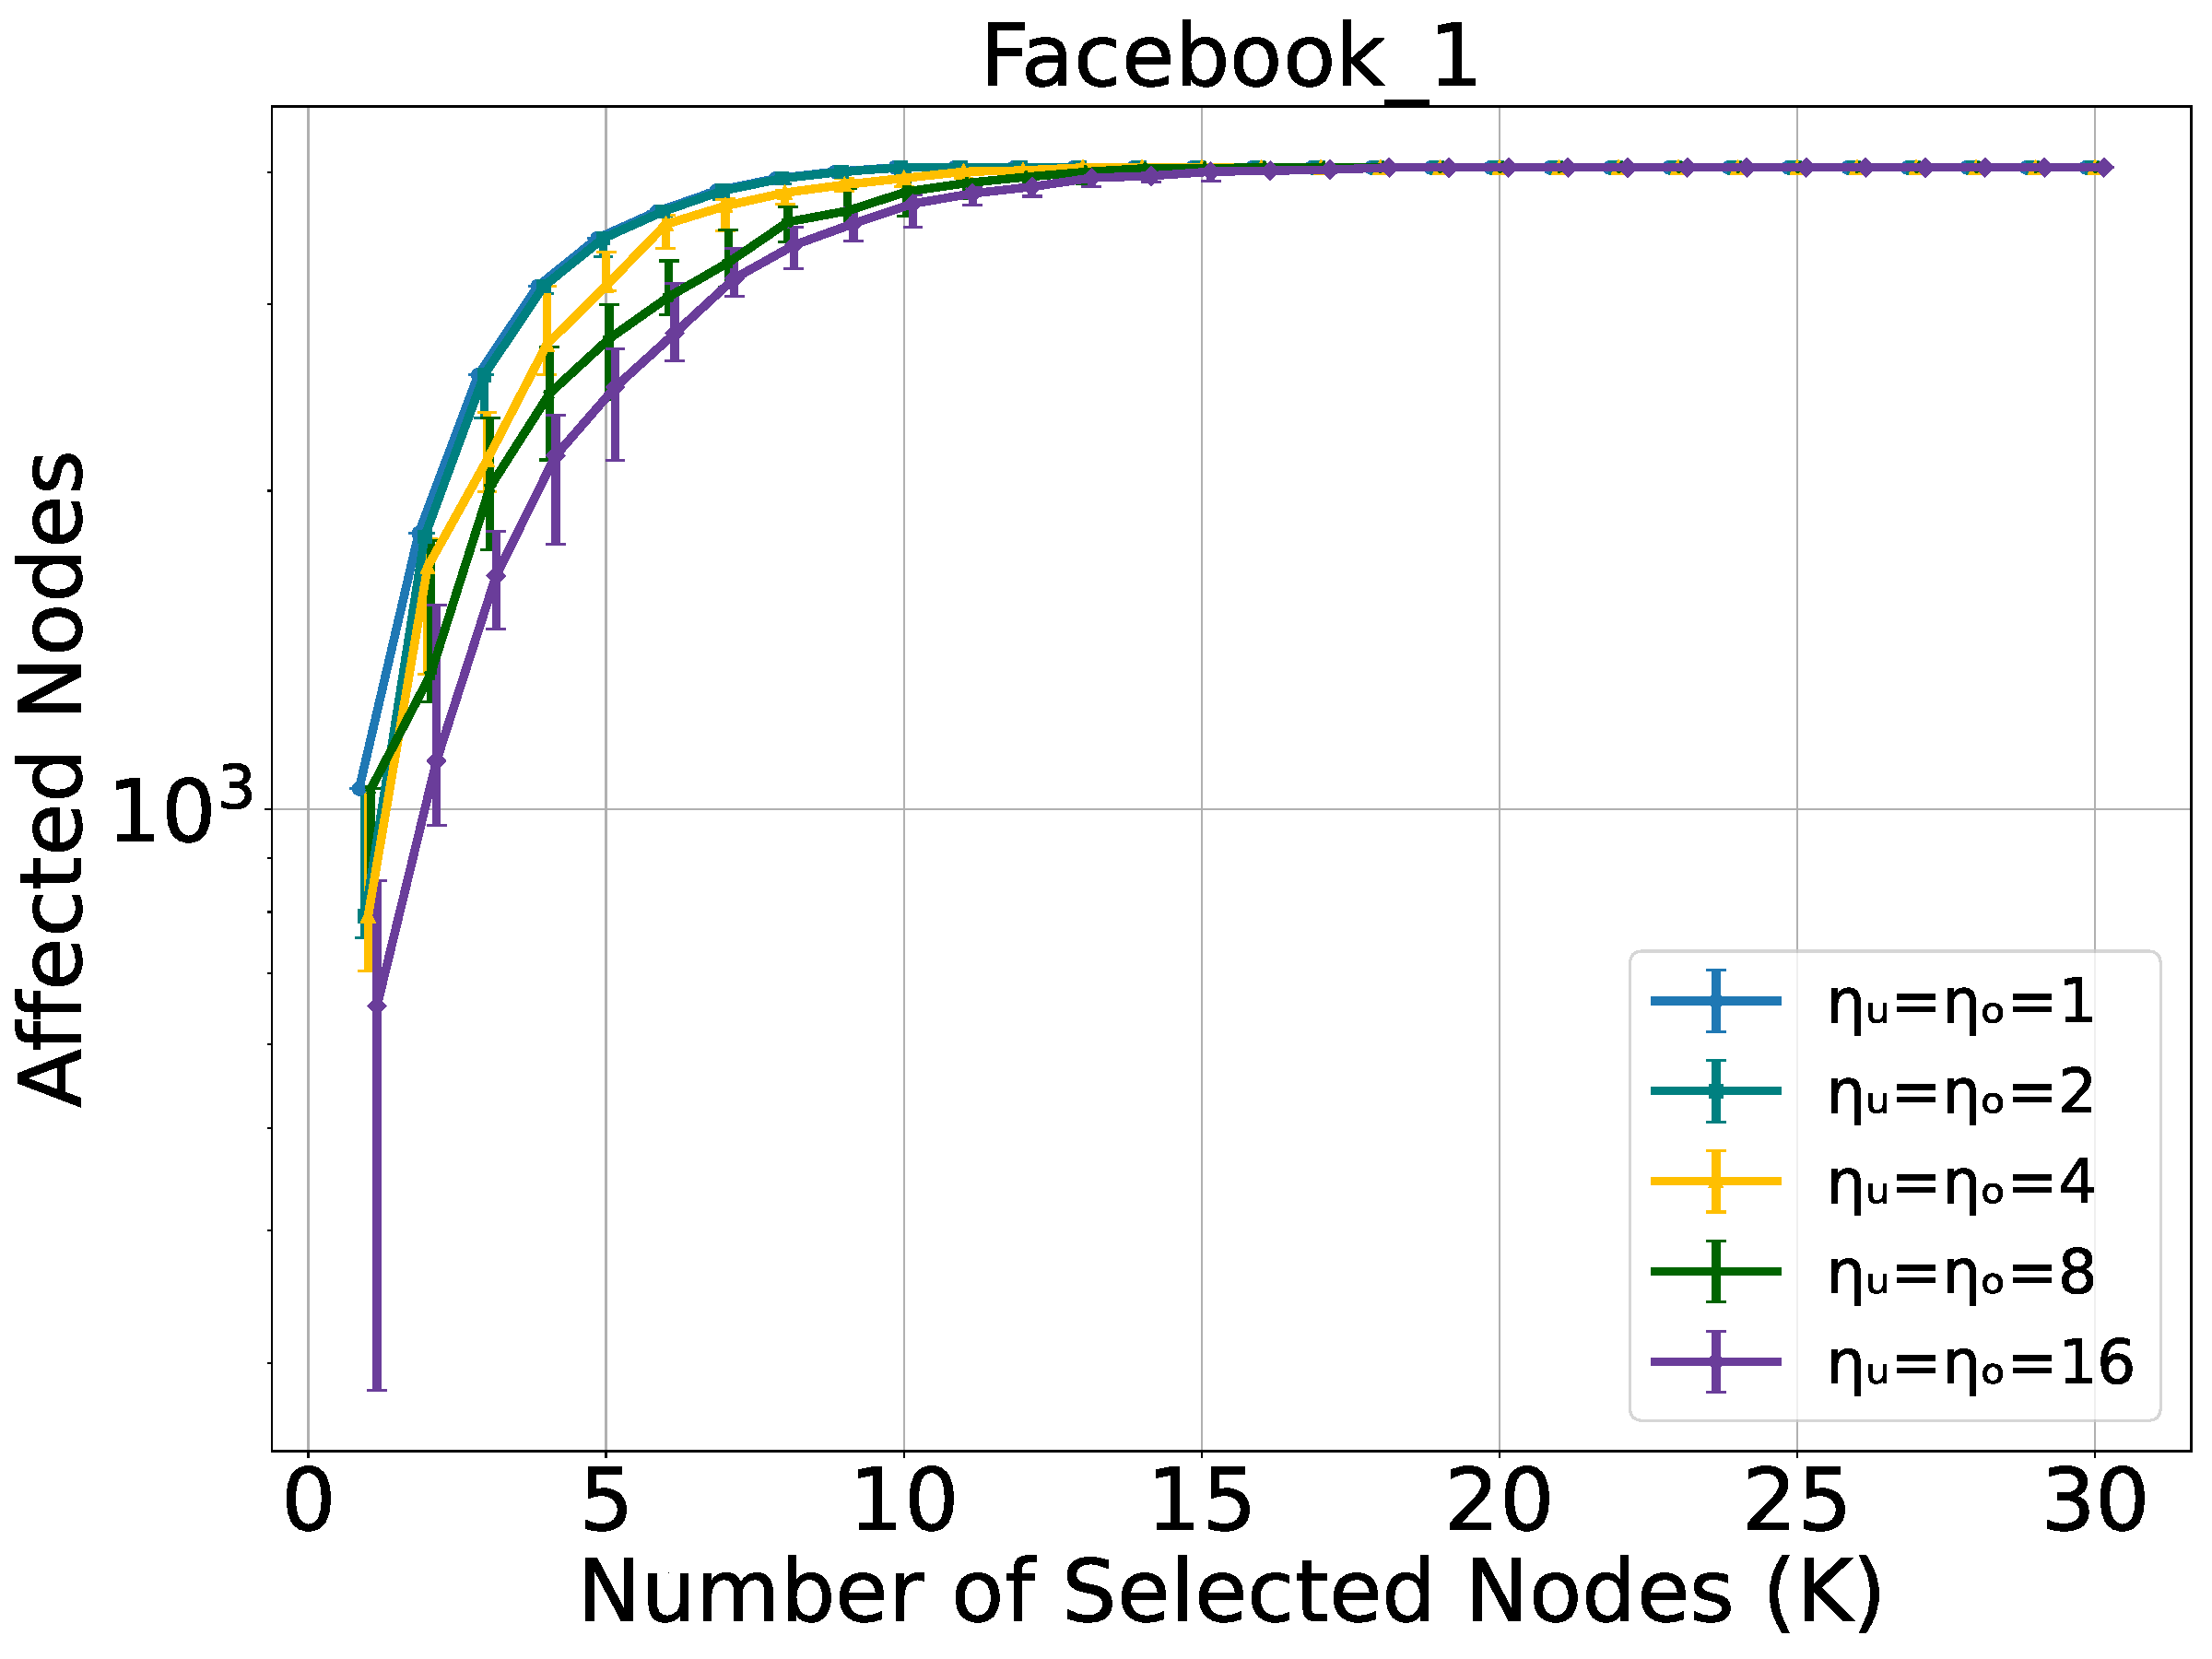
\includegraphics[width=\linewidth]{Figures/GraphExperiment/Errors/new/error_fb1.pdf}
%         \label{fig:error_fb1}
%     \end{minipage}\hfill
%     \begin{minipage}{0.48\columnwidth}
%         \centering
%         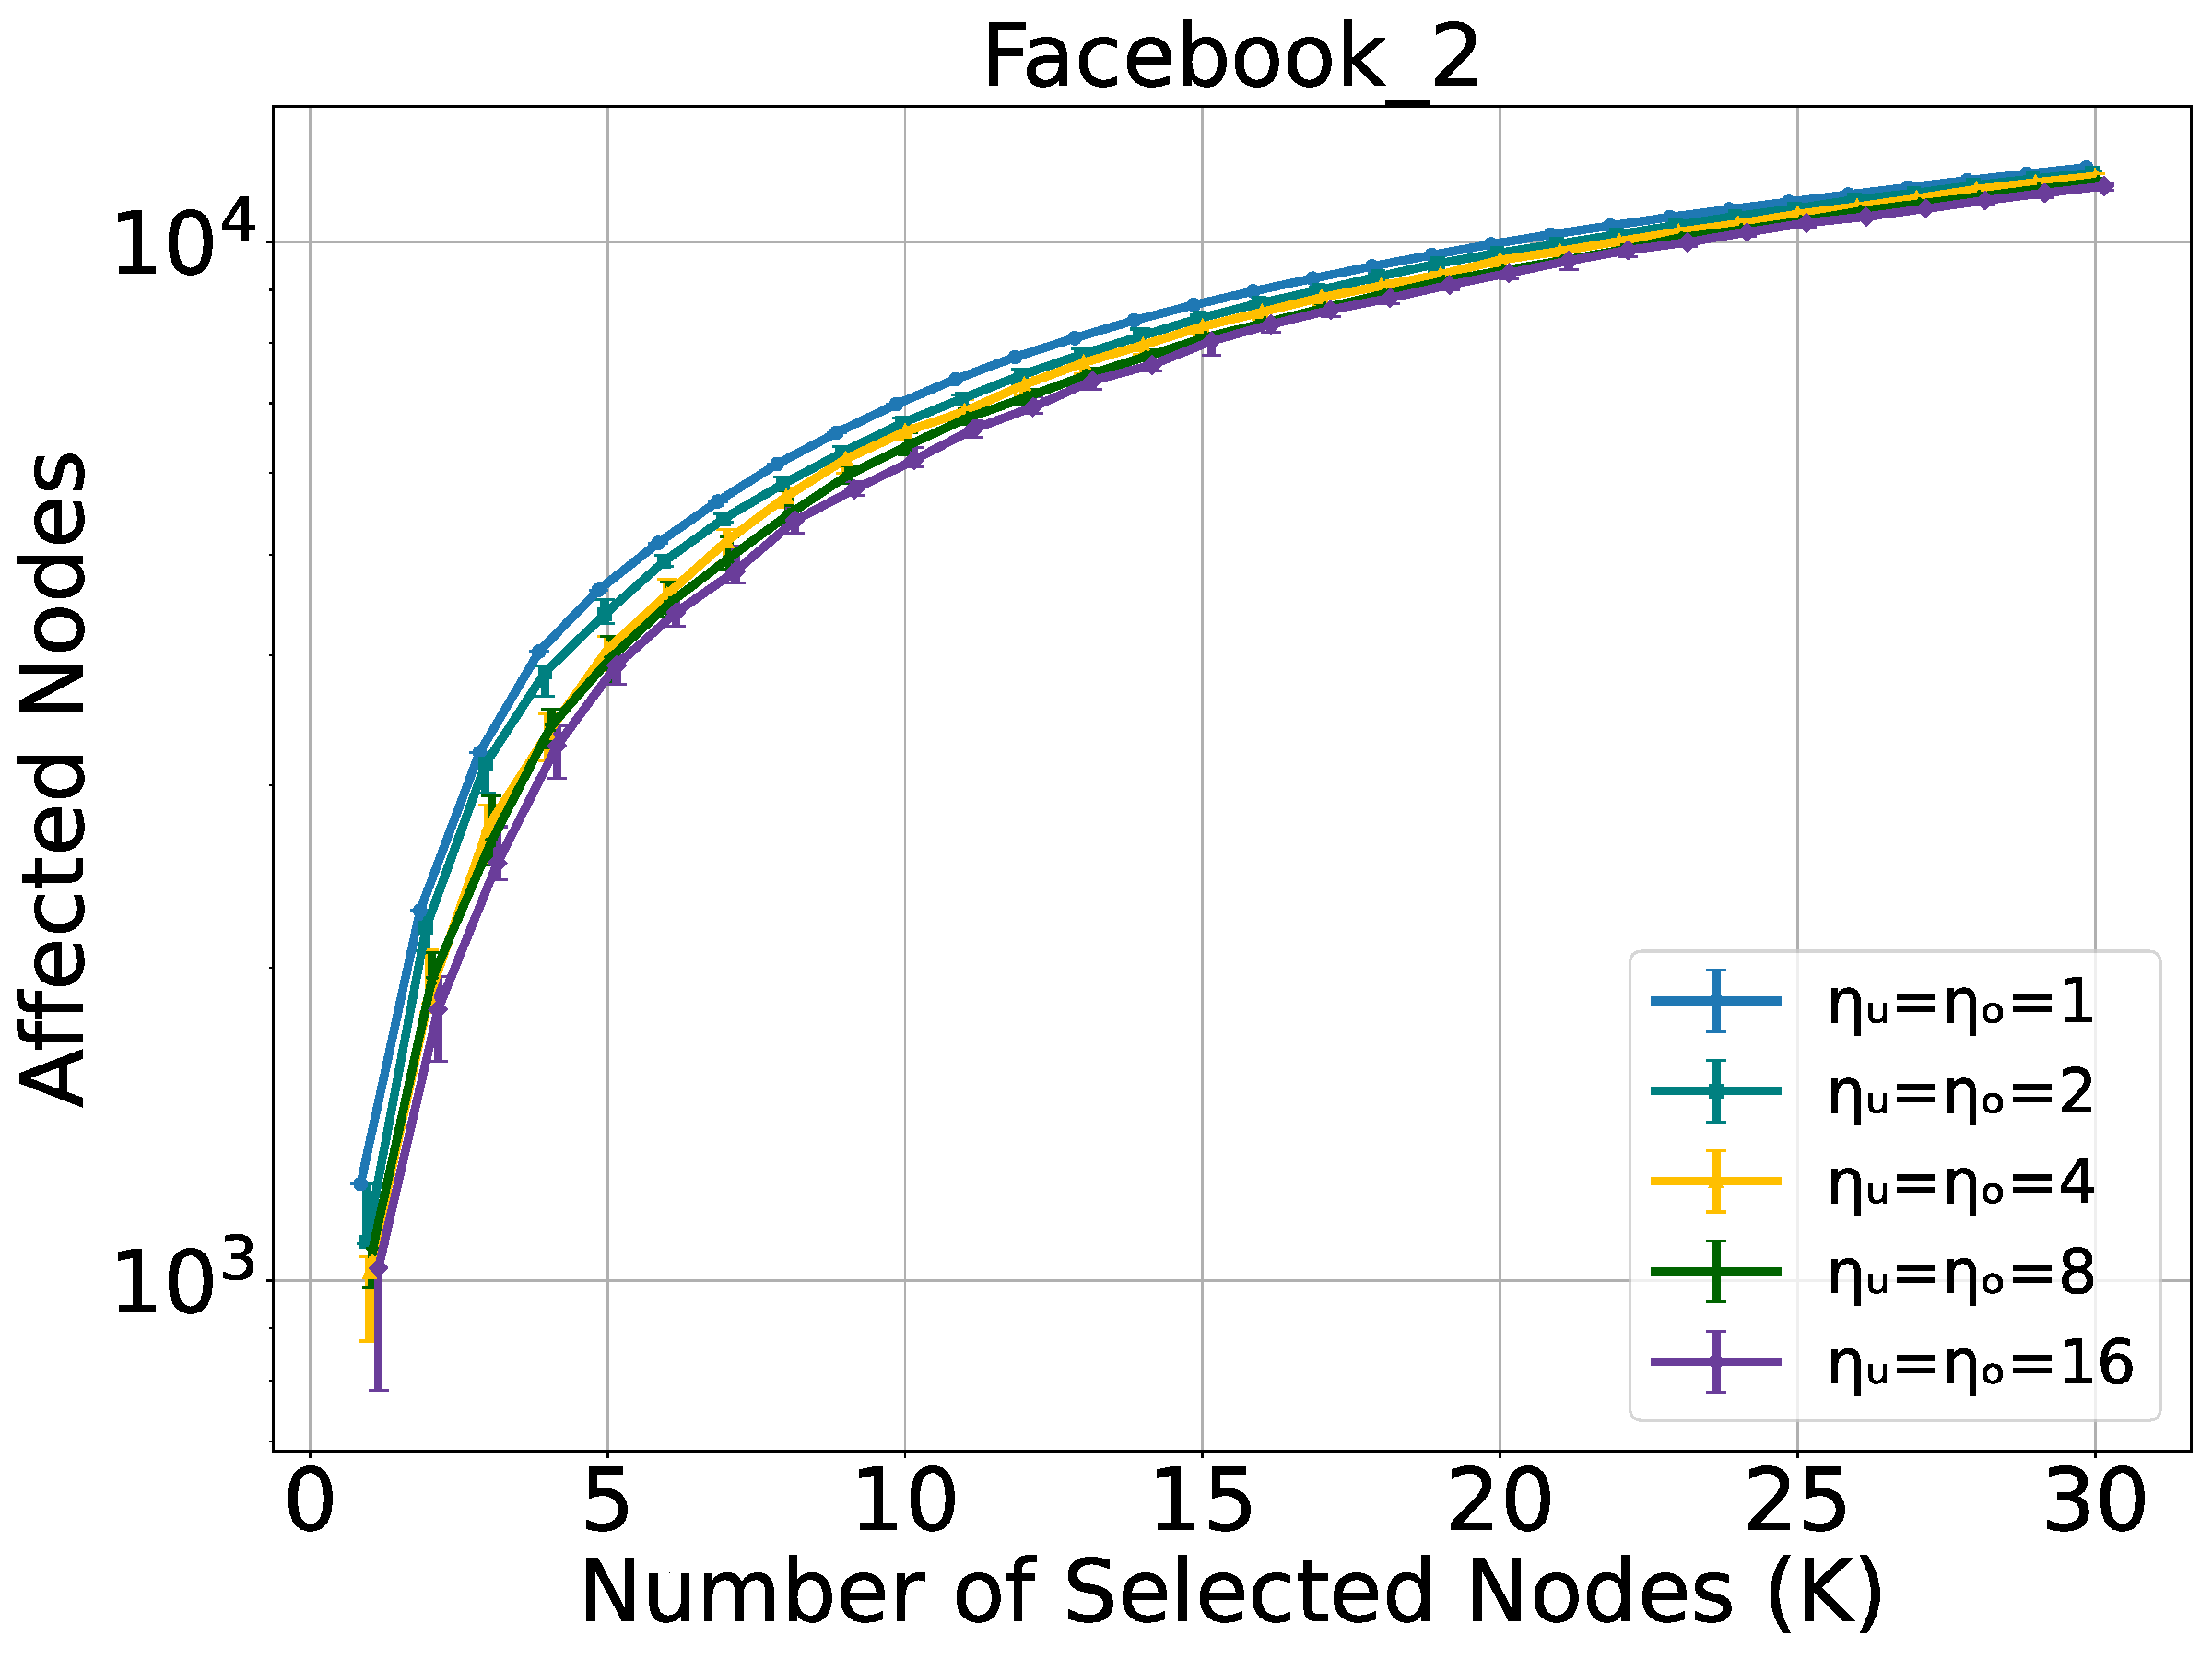
\includegraphics[width=\linewidth]{Figures/GraphExperiment/Errors/new/error_fb2.pdf}
%         \label{fig:error_fb2}
%     \end{minipage}
%     \caption{Affected nodes with an increasing $K$ by SOP-Greedy with $\eta \in [1, 256]$.}
%     \label{fig:graph_error}
% \end{figure}


%Figure \ref{fig:2stp} presents the comparisons between five methodologies: Greedy, SOP-Greedy, RSOP-Greedy, Random, and Weighted Random selection. 
%We only retain 1000 nodes with the largest degrees from each dataset since the complexity of RSOP-Greedy is $O(N^R)$, where $N$ is the number of nodes in the network. Handling large-scale networks makes RSOP-Greedy too slow. 
%Additionally, we perform experiments comparing the other methodologies (excluding RSOP-Greedy) on the large-scale networks. The results of these experiments are shown in Appendix \ref{appendix:large-scale}. 

\textbf{Results.} 
Figure \ref{fig:2stp} shows the empirical performance ratios of different algorithms across four networks with various $K$; the empirical performance ratio is defined as $\frac{f(S_{A})}{\text{OPT}}$, where $S_{A}$ denotes the value of the solution outputted by algorithm $A$ and OPT the (estimated) optimal value. The value of OPT is exact when $K = 1$; for $K > 1$, it is estimated by the solution of the greedy algorithm (with complete information) divided by $1 - e^{-1}$, representing an upper bound for the optimum. Thus, the performance ratios are a lower bound of the actual performance ratios. The empirical performance ratios of the predictive greedy consistently exceed the theoretical bounds, showing the pessimism in our theoretical results and the potential of the proposed algorithm being comparable to optimum in practice. The y-axis is on a logarithmic scale to clarify comparison. Greedy consistently achieves the strongest performance due to complete information. The performance differences between SOP-Greedy and RSOP-Greedy seem insignificant, but Figure \ref{fig:RSOP_C} provides experimental results highlighting their differences. In Figure \ref{fig:2stp}, both exhibit slightly lower performance than Greedy. However, the advantage of Greedy vanishes quickly as $K$ increases. All greedy-based algorithms observe significant advantages over Weighted Random and Random. 




Figure \ref{fig:network visualisation} shows a visualization of the node selection. 
Figure \ref{fig:graph error} presents the performance of SOP-Greedy under different prediction errors. The performance degrades as errors increase, but the disparity diminishes as $K$ increases. We observe that, even under unreasonably large errors, the performance of predictive greedy is competitive even to Greedy with complete information, showing consistency and robustness to the prediction error.


Figure \ref{fig:RSOP_C} shows additional experimental results that compare SOP-Greedy and RSOP-Greedy under various $\eta_u$ and $\eta_o$. The y-axis represents the performance ratio, calculated in the same manner as in Figure \ref{fig:2stp}. Their performance is comparable under accurate predictions. However, as $\eta_u$ and $\eta_o$ increase, RSOP-Greedy demonstrates clear advantages over SOP-Greedy under the same prediction quality. 


\begin{figure}[t]
    \centering
    % First figure
    \begin{minipage}{0.485\textwidth}
        \centering
        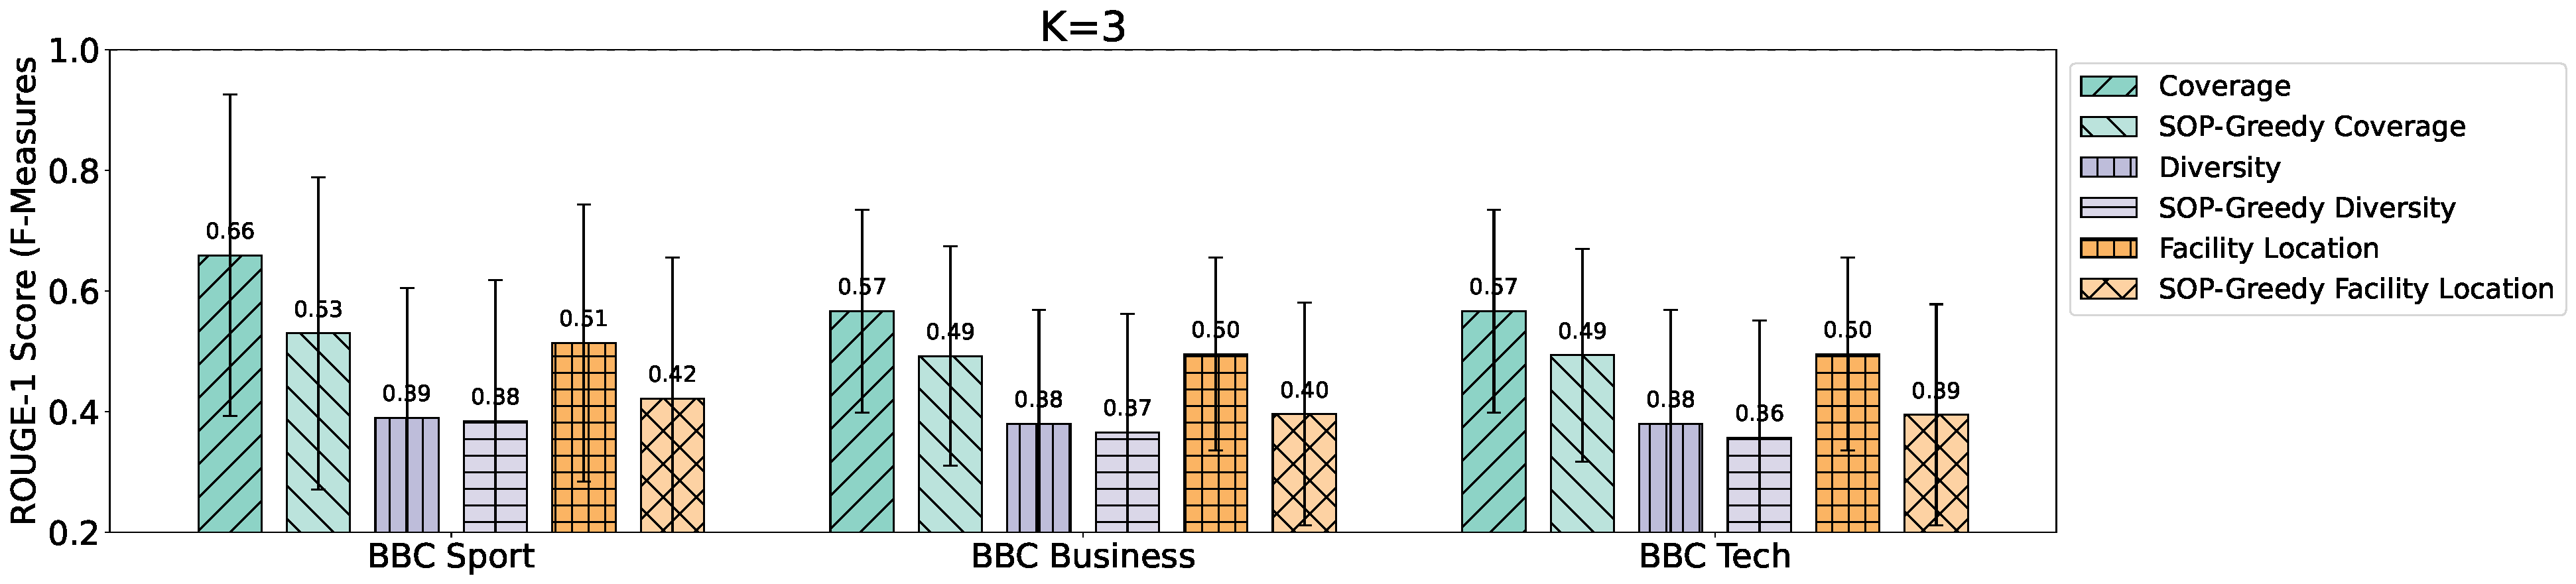
\includegraphics[width=\linewidth]{Figures/experiment 3/bbc_k3.pdf}
        %\\{\tiny (a)}
        \label{fig:bbc_k3_rouge_1}
    \end{minipage}\hfill
    \begin{minipage}{0.485\textwidth}
        \centering
        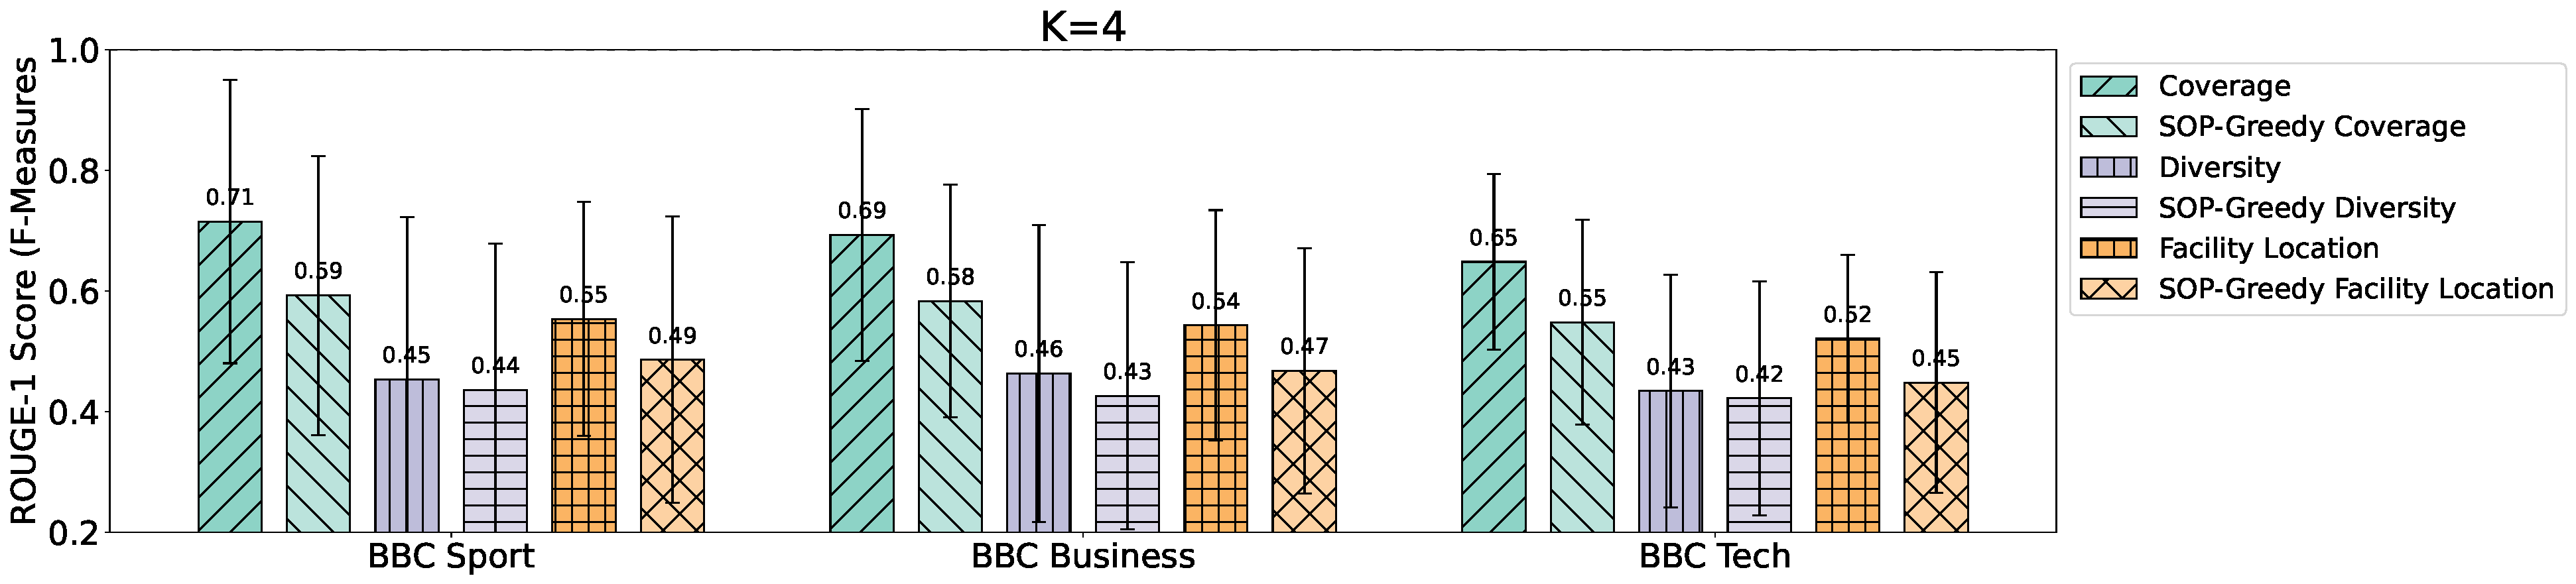
\includegraphics[width=\linewidth]{Figures/experiment 3/bbc_k4.pdf}
        \label{fig:bbc_k4_rouge_1}
    \end{minipage}\hfill
    % Second figure
    \begin{minipage}{0.485\textwidth}
        \centering
        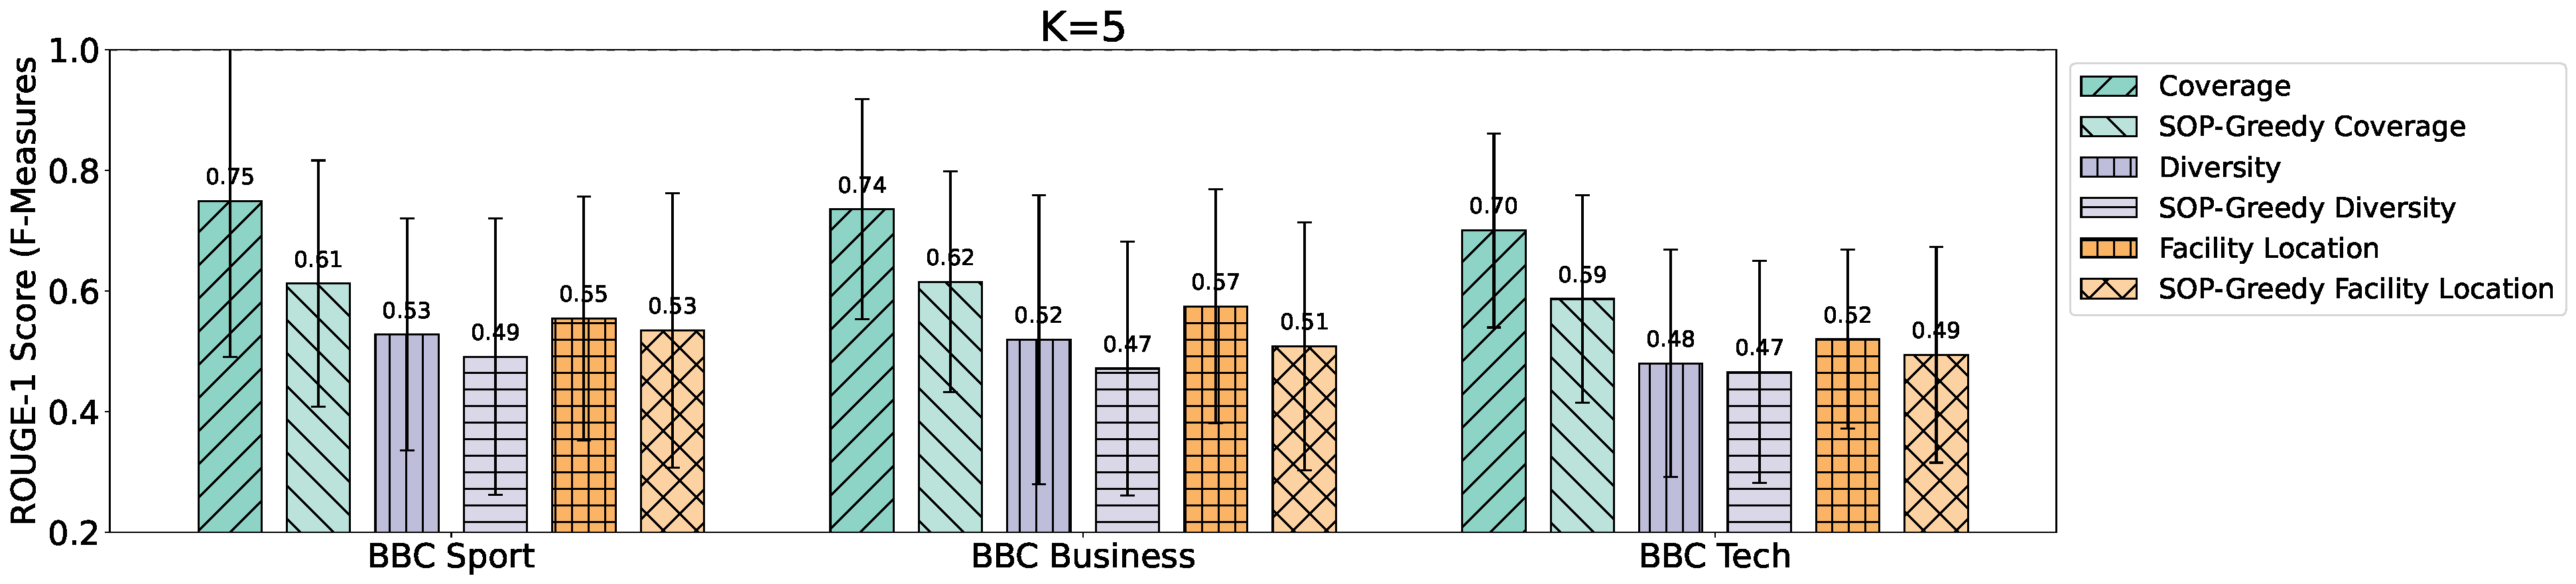
\includegraphics[width=\linewidth]{Figures/experiment 3/bbc_k5.pdf}
        \label{fig:bbc_k5_rouge_1}
    \end{minipage}

    \caption{ROUGE‐1 scores (F‐measure) across three BBC news—sport, business, and tech—under $K \in [3, 5]$. The results highlight how each approach scales with $K$ and differs by BBC news categories \cite{yadav2022extractive}.}
    \label{fig:BBCnews}
\end{figure}




\begin{figure*}[ht!]
    \centering
    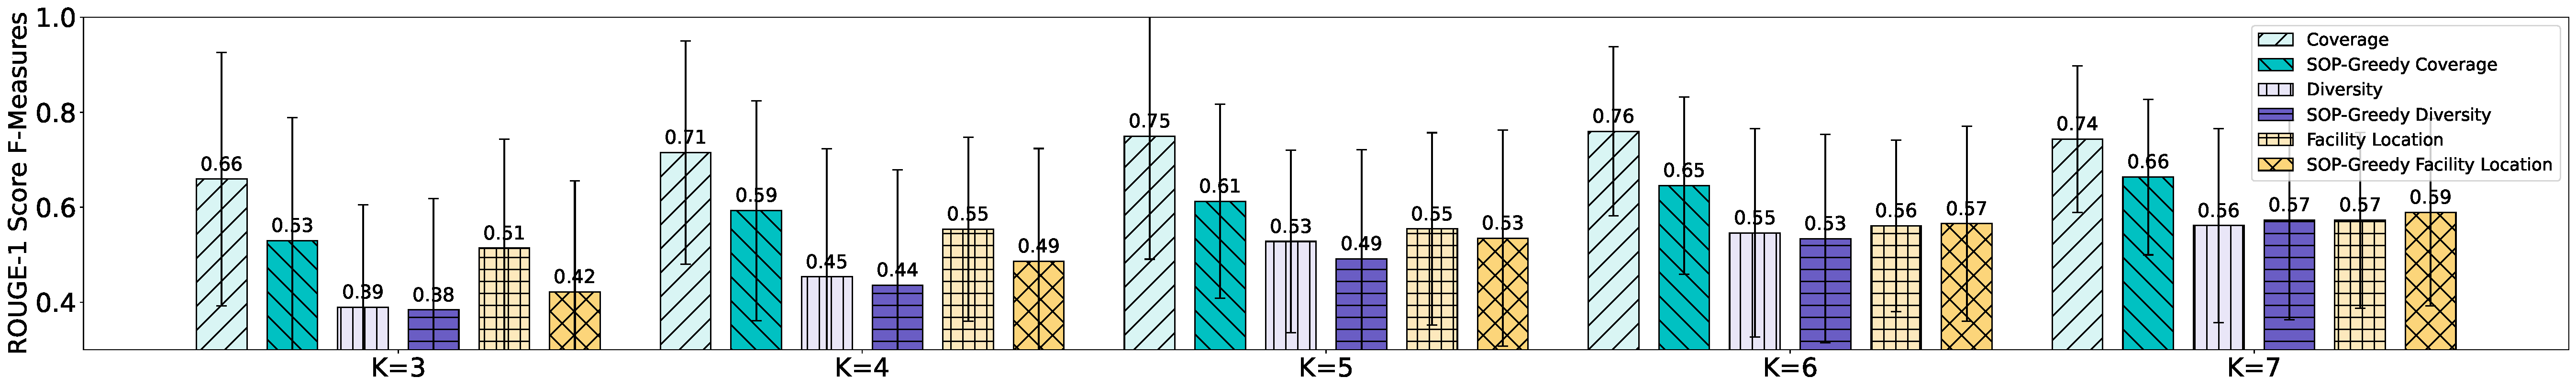
\includegraphics[width=\textwidth]{Figures/experiment 3/sports.pdf}
    \label{fig:dummy-ref}
    \caption{Rouge-1 scores for the greedy and SOP-Greedy under $K \in [3, 7]$ on the BBS news sport \cite{minaee2021deep}. The IQRs of the results are reported.}
    \label{fig:text-summary}
    \vspace{-15pt}
\end{figure*}

\subsection{Text summarization} \label{subsec:text-summarization}


\begin{figure}[t]
    \centering
    % First figure
    \begin{minipage}{0.48\textwidth}
        \centering
        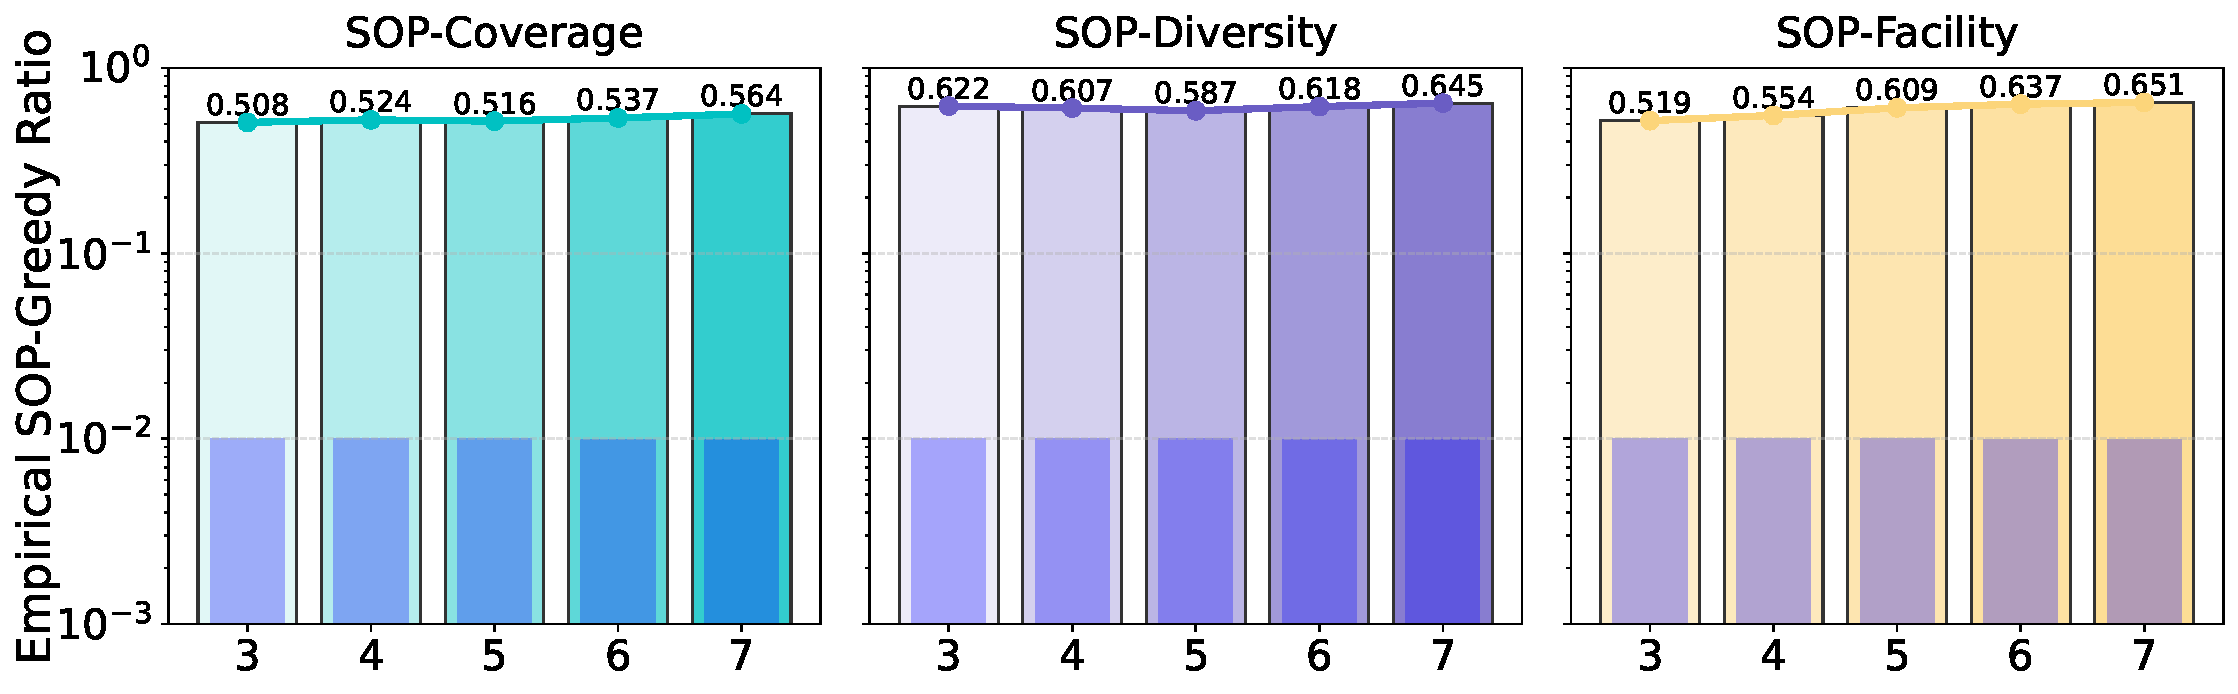
\includegraphics[width=\linewidth]{Figures/experiment 3/performance_ratio.pdf}
        %\\{\tiny (a)}
        \label{fig:sub}
    \end{minipage}\hfill
    
    \caption{Empirical SOP-Greedy performance ratios for text summarization under three submodular objectives—coverage, diversity, and facility—with $K \in [3, 7]$ on the BBS news sport \cite{minaee2021deep}. The bottom shaded bars represent the theoretical bounds.}
    \vspace{-14pt}
    \label{fig:text-ratio}
\end{figure}



This experiment considers text summarization, which has been formulated and proven as submodular optimization under cardinality constraint \cite{lin2011class}. Let $V$ be a set of $n$ tokens, which could be phrases or paragraphs, labeled as $1, \dots, n$, i.e., $V = \{1, \dots, n\}$. Our task is to find a set $S \subseteq V, |S| \leq K$, so that $S$ is a summary of $V$ with the highest quality measured by some score function $f: 2^V \rightarrow \mathbb{R}$. The literature on text summarization proposes many submodular score functions that are widely used. We consider three of them: \textit{coverage}, \textit{diversity}, and \textit{facility location} \cite{lin2011class}. 
Coverage measures information covered and is defined as $f_{\text{cov}}(S) = \sum_{i \in V} \min \left\{\sum_{j \in S} w_{i, j}, \alpha \sum_{k \in V} w_{i, k}\right\}$, where $w_{i, j}$ is the similarity between tokens $i$ and $j$, and $\alpha$ a parameter controlling the saturation point of coverage. 
Diversity measures diversity of the information and is defined as $f_{\text{div}}(S) = \sum_{k=1}^{K} \sqrt{\sum_{j \in S \cap P_k} \frac{1}{N} \sum_{i \in V} w_{i, j}}$, where $S \cap P_k$ denotes the intersection of $S$ with a partition $P_k$ of $V$. 
Facility location measures representativeness to $V$ and is defined as $f_{\text{loc}}(S) = \sum_{i \in V} \max_{j \in S} w_{i, j}$. The text summarization problem can be cast as the following optimization. 

\[ \max_{S \subseteq V} \{f(S) : |S| \leq K, f ~\text{submodular} \} \]

There is no universally agreed $f$. However, it is generally assumed that $f$ is non-decreasing and submodular due to information coverage and redundancy of a summary \cite{lin2011class}, and $f$ correlates well with the ROUGE‐1 score. Though $f$ is inaccessible, practitioners may use a sensible heuristic, such as some variants of the above-mentioned score functions, as the predictor $\tilde{f}$ to approximate ROUGE-1.


%The aim of the third experiment is to extract the most essential information from a lengthy text or collection of documents and present them in a condensed form. 
%We address the issue of extractive summarization as a submodular function maximisation under cardinality constraints, aligning with the methodology given in \cite{lin2011class}. %For monotone submodular functions, greedy algorithms theoretically guarantee near-optimal solutions.

%\textbf{Submodular objective functions.} Every element in our document set, $V = \{1, \dots, n\}$, stands for a separate piece of text, such as a phrase or paragraph, and is used in the context of extractive summarization. 
%Finding a subset $S \subseteq V$ that maximises the summarization quality $F(S)$ while keeping $|S| \leq K$. 
%Here, $F$ is a submodular function that encompasses important factors like coverage, diversity, and facility location, three crucial components in text summarization. 
\begin{comment}
Firstly, the Coverage Function $\mathcal{L}_1(S)$ \cite{lin2011class}, considered as $F_{\text{cov}}(S)$ in our experiment, for maximizing the total information covered by the summary is defined as:
\[
F_{\text{cov}}(S) = \sum_{i \in V} \min \left\{\sum_{j \in S} w_{i, j}, \alpha \sum_{k \in V} w_{i, k}\right\},
\]
where $w_{i, j}$ represents the weight or similarity between elements $i$ and $j$, and $\alpha$ is a parameter to control the saturation point of coverage.

The second submodular function is Diversity Function, $R_1(S)$ \cite{lin2011class}, considered as $F_{\text{div}}(S)$, aims to ensure the summary includes diverse aspects from the document set, expressed as:
\[
F_{\text{div}}(S) = \sum_{k=1}^{K} \sqrt{\sum_{J \in S^{\perp} P_{k}} \frac{1}{N} \sum_{i \in V} w_{i, J}},
\]
where $S^{\perp} P_{k}$ denotes the complement of $S$ within a partition $P_k$ of $V$.

Finally, the Facility Location Function\cite{ahmed2011maximizing}, $F_{\text{loc}}(S)$, focuses on maximizing the representativeness of the subset $S$ for the entire document set:
\[
F_{\text{loc}}(S) = \sum_{i \in V} \max_{j \in S} w_{i, j},
\]
Where the similarity between document $i$ and phrase $j$ in the subset $S$ is denoted by $w_{i, j}$.
\end{comment}

\begin{comment}
Then we modify the standard greedy submodular maximization algorithm by incorporating a prediction error term:

    \[
    f_{\text{error}}(S) = f(S) + \epsilon(S), \quad \epsilon(S) \sim \mathcal{U}(-\log \eta_u, \log \eta_o),
    \]
where $\epsilon(S)$ models the error as a uniformly distributed variable.
\end{comment}

\textbf{Experimental set-up.}
We collect texts from BBC news \cite{bbcnews_dataset} to form three datasets each including 100 articles under sport, business, and tech categories. Every article is tokenized into sentences. Every article has its summary from BBC news. We evaluate the summarization algorithm using the original summary with Rouge-1 score F-measure, a metric that balances information relevance and accuracy. We implement the greedy algorithm and predictive greedy. The greedy algorithm uses coverage with $\alpha$ = 1, diversity with number of clusters = 2, and facility location as heuristic to determine the summary; the feature extraction step employs IDF-weighted term vectors; the predictive greedy uses an erroneous heuristic. We want to see how the errors in the heuristic affect the quality of the summary measured by Rouge-1 score against the original summary. 
The algorithm is evaluated with different heuristics; the cardinality constraint $K$ ranges from 3 to 7; the prediction error is set to $\eta = 100$ ($\eta_u = \eta_o = 10$). The experiments are conducted with Intel Core 12600KF, RAM 16GB, and GPU Nvidia Geforce RTX 3070, 8GB VRAM. 


\textbf{Results.}
Across the three BBC news categories, as shown in Figure \ref{fig:BBCnews}, coverage and facility consistently achieve higher ROUGE-1 scores than diversity, while predictive greedy behaves similarly to greedy algorithms with complete information. Figure \ref{fig:text-summary} shows the Rouge-1 scores for three submodular heuristics—coverage, diversity, and facility—under varying $K$ on the BBS news sport dataset. The performance of the greedy and predictive greedy converges as $K$ increases, showing the consistency and robustness of the predictive greedy under large $K$. Diversity is the worst among the three heuristics for summarization under small $K$. This is intuitive, as information coverage is the primary concern and diversity is secondary. Figure \ref{fig:text-ratio} shows the empirical performance ratios of SOP-Greedy, estimated with OPT set to $\min \{ 1, \frac{f(S_{\text{greedy}})}{1 - e^{-1}}\}$, where $S_{\text{greedy}}$ denotes the solution outputted by the greedy with complete information. The non-trivial error ($\eta_u = \eta_o = 10$) leads to minor theoretical bounds, shown in Figure \ref{fig:text-ratio} and Table \ref{tab:theoretical-bound}. The empirical performance ratios are consistently higher than the competitive ratios, showing the potential of the predictive greedy to be close to the optimum in practice. 

\begin{table}[ht!]
\centering
\caption{Competitive ratios for SOP-Greedy under varying K and $\eta_u = \eta_o = 10$.}
\label{tab:theoretical-bound}
\begin{tabular}{c|ccccc}
\hline\hline
\textbf{K} & 3 & 4 & 5 & 6 & 7 \\
\hline
\textbf{comp. ratio} & 0.009967 & 0.009963 & 0.009960 & 0.009958 & 0.009957 \\
%\textbf{K} & \textbf{SOP-Coverage} & \textbf{SOP-Diversity} & \textbf{SOP-Facility Location} \\
%\hline
%\textbf{3}   & 0.009967 & 0.009967 & 0.009967 \\
%\textbf{4}   & 0.009963 & 0.009963 & 0.009963 \\
%\textbf{5}   & 0.009960 & 0.009960 & 0.009960 \\
%\textbf{6}   & 0.009958 & 0.009958 & 0.009958 \\
%\textbf{7}   & 0.009957 & 0.009957 & 0.009957 \\
\hline\hline
\end{tabular}
\vspace{-12pt}
\end{table}

%It is observed in Figure \ref{fig:textk}: when K increases, the Rouge-1 score also improves because adding sentences in the simulated summary bring audience with valid information. 
%When K reaches a certain point, K = 5, the incremental information gain is not obvious. So, we make the subsequent plots across three news categories for K = 3, 4 and 5, which is displayed in Appendix \ref{appendix:supp-material-application3}. 
%Figure\ref{fig:overall} indicates that converge and facility location greedy have similar performance and outperform the other method. The predictive greedy has close performance with each objective method under the reasonable prediction error value. These findings support the statement that submodular functions, especially when implemented with predictive error, offer a robust structure for producing short but informative summaries. Consistent performance across different $K$ values further demonstrates how the predictive methods can be adjusted for various cardinaity constraints. 


\begin{comment}
\begin{figure}
    \centering
    \begin{subfigure}{\textwidth}
        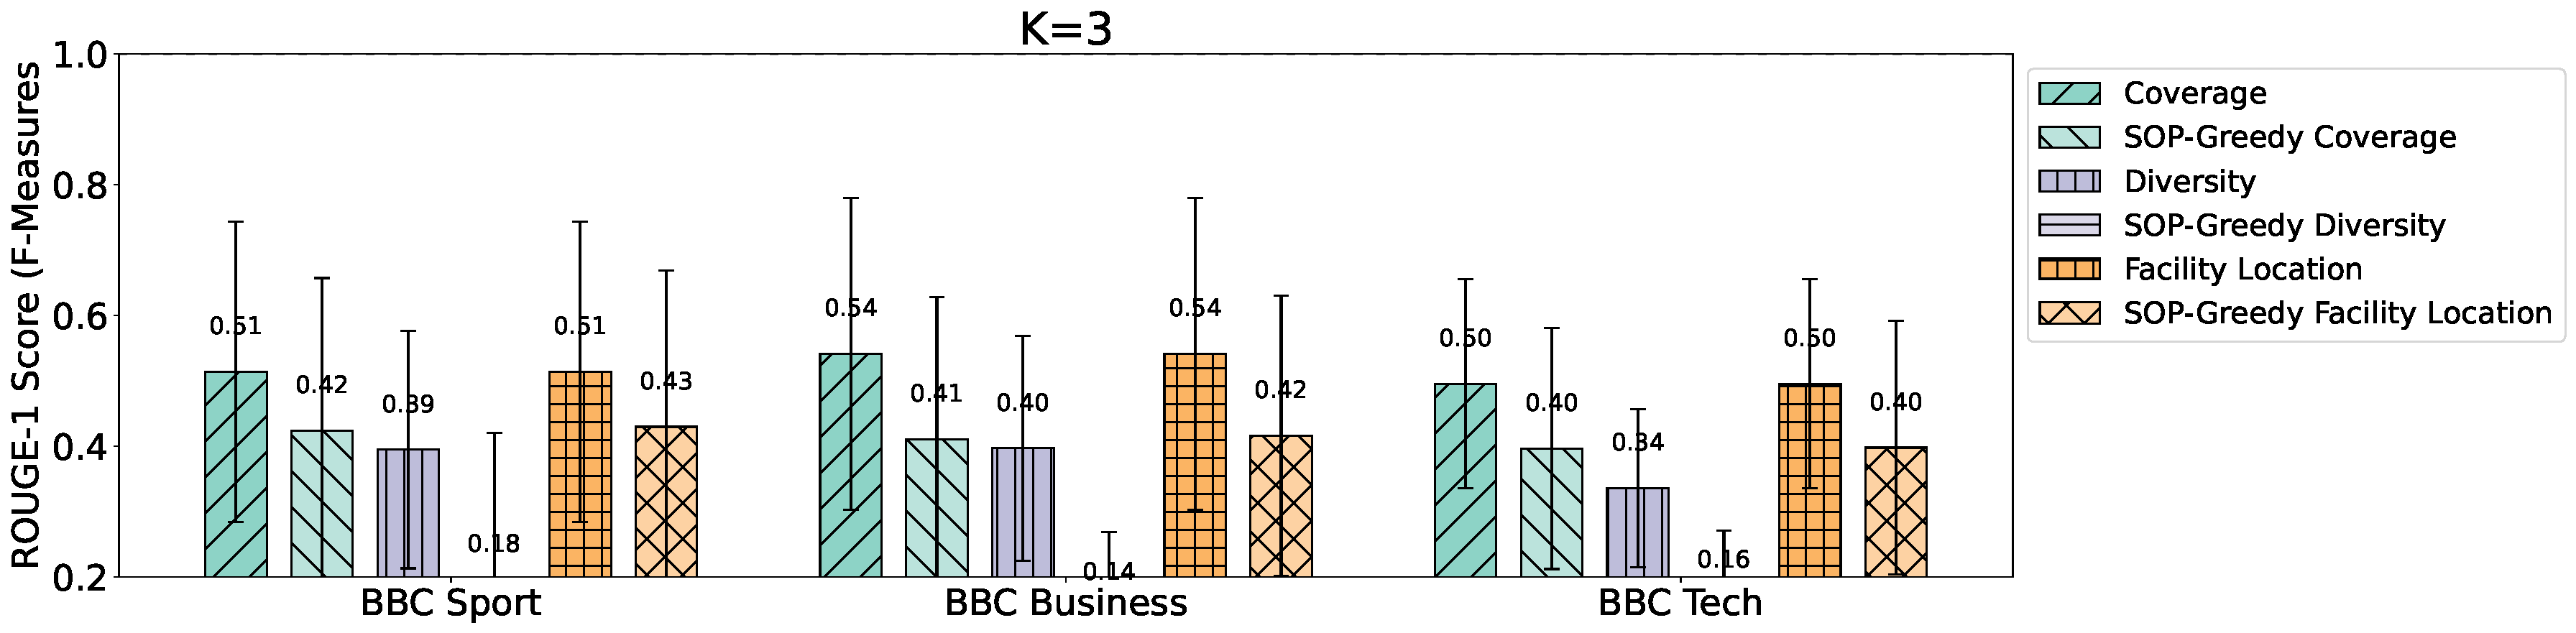
\includegraphics[width=0.65\textwidth]{Figures/experiment 3/bbcsport_k3.pdf}
    \end{subfigure}
    \begin{subfigure}{\textwidth}
        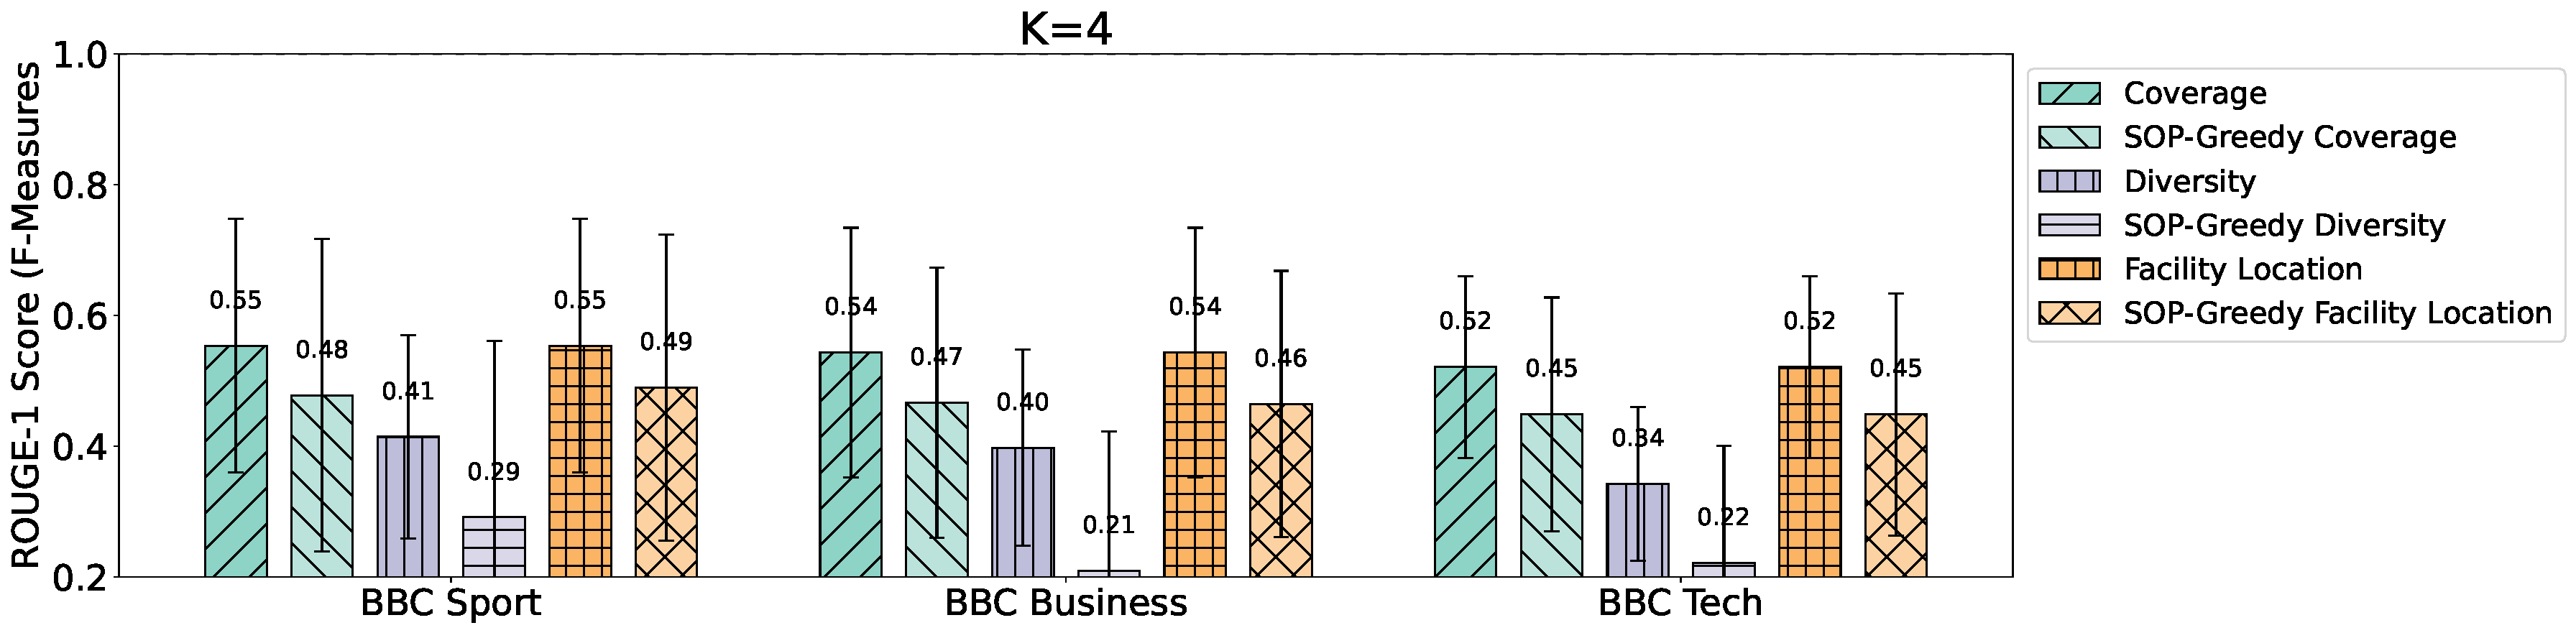
\includegraphics[width=0.65\textwidth]{Figures/experiment 3/bbcsport_k4.pdf}
    \end{subfigure}
    \caption{Overall Caption for all Plots}
    \label{fig:overall}
\end{figure}
\end{comment}


\subsection{Concluding remarks}
Our experiments show that SOP-Greedy and RSOP-Greedy are robust to prediction errors when $\eta$ is up to hundreds in real-world applications. They observe performance comparable to the greedy with complete information and smooth and graceful performance degradation as prediction errors worsen. These results also verify the theoretical guarantees, even if we use the upper bounds of OPT in the calculation. 


